%\documentclass{amsart}
\documentclass[12pt,a4paper,oneside]{book}
%     If your article includes graphics, uncomment this command.
\usepackage{amsthm}
\usepackage{amssymb}
\usepackage[brazilian]{babel}
\usepackage[utf8]{inputenc}
\usepackage[T1]{fontenc}

\usepackage{geometry}
\usepackage{dirtytalk}
\usepackage{mathtools}
\usepackage{epigraph}
\usepackage{comment}
\usepackage{float}
\usepackage{soul}
\usepackage{subfig}
%\usepackage{subcaption}
\usepackage{tcolorbox}
\usepackage{xcolor}
\usepackage[colorlinks  = true,
            linkcolor   = blue,
            urlcolor    = blue,
            citecolor   = blue,
            anchorcolor = blue]{hyperref}

\usepackage{multicol}
\usepackage{makeidx}
\makeindex


\geometry{margin=1.2in}
\newtheorem{theorem}{Teorema}[section]
\newtheorem{proposition}[theorem]{Proposi\c{c}\~ao}
\newtheorem{corollary}[theorem]{Corol\'ario}
\newtheorem{lemma}[theorem]{Lema}
\newenvironment{claim}[1]{\par\noindent\underline{Afirma\c{c}\~ao:}\space#1}{}
\newenvironment{claimproof}[1]{\par\noindent\underline{Prova da afirma\c{c}\~ao:}\space#1}{\hfill $\square$}

\theoremstyle{definition}
\newtheorem{definition}[theorem]{Defini\c{c}\~ao}
\newtheorem{example}[theorem]{Exemplo}
\newtheorem{fato}[theorem]{Fato}
\newtheorem{xca}[theorem]{Exerc\'icio}

\theoremstyle{remark}
\newtheorem{remark}[theorem]{Observa\c{c}\~ao}

\numberwithin{equation}{section}

%    Absolute value notation
\newcommand{\abs}[1]{\lvert#1\rvert}

%    Blank box placeholder for figures (to avoid requiring any
%    particular graphics capabilities for printing this document).

\newcommand{\R}{\mathbb{R}}
\newcommand{\e}{\varepsilon}
\newcommand{\N}{\mathbb{N}}
\newcommand{\E}{\mathbb{E}}
\newcommand{\pr}{\mathbb{P}}
\newcommand{\ds}{\displaystyle}
\newcommand{\Var}{\mathbb{V}\text{ar}}
\newcommand{\Cov}{\textrm{Cov}}
\newcommand{\rarrowlimn}{\xrightarrow{n\rightarrow \infty}}
\newcommand{\F}{\mathcal{F}}

\renewcommand\qedsymbol{$\blacksquare$}

\begin{document}

\title{{\Huge Introdução à Probabilidade}}

%    Information for first author
\author{Thiago Ramos}
%    General info

\maketitle


\section*{Licença}

© 2024 Thiago Rodrigo Ramos. \\
Todos os direitos reservados. Permitido o uso nos termos da licença Creative Commons Atribuição-CompartilhaIgual 4.0 Internacional. \\
\href{https://creativecommons.org/licenses/by-sa/4.0/}{Reutilização deste material}

Você pode remixar, transformar, e criar a partir do material para qualquer fim, mesmo que comercial. Nesse caso, tem de distribuir as suas contribuições sob a mesma licença que o original. Você não pode aplicar termos jurídicos ou medidas de caráter tecnológico que restrinjam legalmente outros de fazerem algo que a licença permita.


\noindent\textbf{Atribuição} \\
Este material foi produzido originalmente por Thiago Rodrigo Ramos (UFSCar).


\noindent\textbf{Código-fonte} \\
O código-fonte deste material está disponível em:
\url{https://github.com/thiagorr162/notas-de-aula}


\noindent\textbf{Aviso legal} \\
As pessoas e instituições aqui mencionadas não endossam a qualidade deste material e as opiniões nele contido, nem explícita nem implicitamente. Qualquer erro contido neste material é responsabilidade de: Thiago Rodrigo Ramos.

\vspace{5em}
\date{\today}

\newpage


\tableofcontents
\newpage 

\newpage


\section*{Legenda das Caixas}


\begin{tcolorbox}
Caixas desta cor representam resultados importantes, como teoremas, exemplos, etc.
\end{tcolorbox}

\begin{tcolorbox}[colback = yellow!70]
Caixas desta cor representam observações importantes, como intuição dos problemas, conexões com outros resultados, etc.
\end{tcolorbox}



\chapter{Introdução à Probabilidade  }

\begin{tcolorbox}[colback = white]
As Principais referências usadas foram:
\begin{enumerate}
\item \cite{durrett}
\item \cite{spencer-probMethod}
\item \cite{knill}
%\item \cite{chung}
\item \cite{stoyanov2014counterexamples}
\end{enumerate}

\end{tcolorbox}

\section{Teoria da Medida}


\begin{definition}[$\pi$-System] \index{System!$\pi$} Uma família de conjuntos $\mathcal{F}\subset \Omega$ é um $\pi$-system se para todo $A,B\in \mathcal{F}$, temos que $A\cap B\in \mathcal{F}.$

\end{definition}





\begin{definition}[$\lambda$-System/ Dynkin System] \index{System!$\lambda$}\index{System!Dynkin}  Uma família de conjuntos $\mathcal{F}\subset \Omega$ é um $\lambda$-System  (ou Dynkin-System) se :
\begin{enumerate}
\item $\Omega\in \mathcal{F}$.
\item Se $A,B\in \mathcal{F}$ e $A\subset B$, então $B-A\in \mathcal{F}.$
\item Se $(A_n)\subset \mathcal{F}$ e  $A_n\uparrow A$ então $A\in \mathcal{F}.$
\end{enumerate}

Além disso, vamos dizer que $\mathcal{F}\subset \Omega$ é um $\pi$-$\lambda$-system se este for um $\pi$-system e um $\lambda$-system.
\end{definition}

\begin{remark}
É claro que toda $\sigma$-álgebra é um $\pi$-system e um $\lambda$-system.
\end{remark}

\begin{lemma}
Temos que $\mathcal{F}$ é uma $\sigma$-álgebra em $\Omega$ se, e somente  se, $\mathcal{F}\subset \Omega$ é um $\pi$-$\lambda$-system. \index{System!$\pi$-$\lambda$}
\end{lemma}

\begin{proof}
A ida é trivial. Suponha que $\mathcal{F}$ é um $\pi$-$\lambda$-system, vamos mostrar que $\mathcal{F}$ é uma $\sigma$-álgebra.

Como $\mathcal{F}$ é um $\pi$-system, então $\Omega\in \mathcal{F}$ e como $\mathcal{F}$ é um $\lambda$-system, então se $A\in \mathcal{F}$, temos que $A^c = \Omega-A\in \mathcal{F} $. Além disso, dados $A,B\in \mathcal{F}$, temos que $A\cup B = (A^c\cap B^c)^c\in \mathcal{F}$, logo $\mathcal{F}$ também é fechado por uniões finitas, mas como é um $\lambda$-system, tomando $B_n = \cup^n_i A_i\in \mathcal{F}$, temos o resultado, já que $B_n\uparrow \cup A_n$.

\end{proof}

\begin{definition}
Considere a família de subconjuntos $\mathcal{F}\subset \Omega$. Então $\lambda(\mathcal{F})$ é o menor $\lambda$-system contendo $\mathcal{F}$. 

Dizemos que $\lambda(\mathcal{F})$ é o $\lambda$-system gerado por $\mathcal{F}$.
\end{definition}

\begin{lemma}
Se $\F$ é um $\pi$-system, então  $\lambda(\F) = \sigma(\F)$.
\end{lemma}
\begin{proof}
É claro que $\sigma(\F)$ é um $\lambda$-system para $\F$ e então,
$$\lambda(\F)\subset \sigma(\F). $$
Portanto, se mostrarmos que $\lambda(\F)$ é um $\pi-\lambda$-system, pelo lema anterior vamos ter que $\lambda(\F)$ é uma $\sigma$-álgebra, logo 
$$\sigma(\F)\subset \lambda(\F) \subset \sigma(\F), $$ concluindo o resultado.

Vamos mostrar então que $\lambda(\F)$ é $\pi$-system, já que claramente já é $\lambda$-system.


\[:= \coloneqq\]

\end{proof}



\newpage

\section{Resultados Básicos}








\begin{example}[Uma relação importante] Suponha que $\E(|X|)<\infty.$ Sabemos que se $X\geq 0 $ tem densidade $f_X$ então
$$\E(X) = \int_0^\infty xf_X(x)dx $$
mas entao, se $F_X(t) = \pr(X\leq t)$ é a cumulativa de  $X$, como $f_X(t) = F_X'(t)$ temos que
\begin{align*}
\E(X) &= \int_0^a xf_X(x)dx\\
 	&= -\int_0^a F_X(t)dt +  aF_X(a) \\
 	&= a-\int_0^a F_X(t)dt -a +  aF_X(a)\\
 	&= \int_0^a1- F_X(t)dt +  a(F_X(a)-1)\\
  	&= \int_0^a P(X>t)dt +  a(F_X(a)-1).
\end{align*}
Tomando o limite $a\rightarrow +\infty$ temos que  $a(F_X(a)-1) \rightarrow 0$, já que
$$ a(F_X(a)-1) = a\pr(X>a)\leq \E(X1_{X>a})\rightarrow 0,$$
pelo Teorema da Convergência Dominada (lembre-se que pedimos que $\E(|X|)<\infty$). 
Ficamos então com 
$$\E(X) =\int_0^\infty P(X>t)dt. $$
Essa relação fica bem clara no caso discreto, já que temos
$$ 
\begin{array}{cccccccccccccccccccc}
\int_0^\infty P(X>t)dt &= \pr(X=1) &+ \pr(X=2) &+\pr(X=3) &+ \cdots\\
      &0   &+ \pr(X=2) &+\pr(X=3) &+ \cdots\\
      &\vdots&\\
      &= \pr(X=1) &+ 2\pr(X=2) &+ 3\pr(X=3) &+ \cdots\\
      &=& \int_0^\infty xP(X=x) = \E(X).

\end{array}
$$

\end{example}


\begin{tcolorbox}
\begin{example}[Desigualdade Triangular para Probabilidades] Vamos mostrar que
$$\pr(|X-Y|>\e)\leq \pr(|X|>\e/2) +\pr(|Y|>\e/2), $$
isto é, que
$$\{|X-Y|>\e\} \subset \{|X|>\e/2\}\cup \{|Y|>\e/2\}. $$
Para isso, suponha  que vale $\{|X-Y|>\e\}$ mas  não $\{|X|>\e/2\}$, isto é,  $\{|X|\leq\e/2\}$. 

Como
$$|X|+|Y|\geq |X-Y|>  \e, $$ temos que
$$|Y| > \e - \e/2 = \e/2, $$
concluindo o resultado.
\end{example}
\end{tcolorbox}


\newpage


\section{Distribuições}\label{section- distribuicoes}

%\begin{definition}[Função Cumulativa de Distribuição - variáveis aleatórias]

%\end{definition}



\index{Distribuição}
\begin{theorem} Seja $X$ uma v.a. e $F$ sua distribuição. Então
\begin{enumerate}
\item $F$ é não decrescente.
\item Temos que
$$\lim_{x\rightarrow +\infty} F(x) = 1$$ e que
$$\lim_{x\rightarrow -\infty} F(x) = 0.$$
\item $F$ é contínua à direita, isto é,
$$\lim_{y\downarrow x}F(y) = F(X). $$
\item Se $F(x-) = \lim_{y\uparrow x}F(y)$, então 
$$F(x-) = \pr(X<x). $$ 
\item Temos que
$$ \pr(X=x) = F(x)-F(x-).$$
\item $F$ tem no máximo uma quantidade enumerável de descontinuidades.
\end{enumerate}

\end{theorem}

\begin{proof}
Vamos provar cada item separadamente.
\begin{enumerate}
\item Se $x< y$, então
$$F(y)= \pr(X\leq y) = \pr(X\leq x) + \pr(x < X\leq y )\geq \pr(X\leq x)= F(x). $$
\item Note que  a família de eventos
$\{X\leq n\}$
é crescente e que 
$$\bigcup_{i=1}^n \{X\leq i\} = \Omega. $$
\item Note que, se $y_n\downarrow x$, então a família de eventos $\{X\leq y_n\}$ é decrescente e que 
$$\bigcap_{i=1}^n\{X\leq y_i\}= \{X\leq x\}. $$
\item Note que,se $y_n\uparrow x$, então a família de eventos $\{X\leq y_n\}$ é crescente e que 
$$\bigcup_{i=1}^n\{X\leq y_i\}= \{X< x\}. $$ 
\item Basta notar que
$$\pr(X=x) = \pr(X\leq x)- \pr(X<x), $$
e usar os itens anteriores.
\item Para cada descontinuidade $x$ de $F$, temos que
$$F(x-)-F(x+)>0, $$
tome então $q_x\in \mathbb{Q}$ tal que  $F(x-)<q_x<F(x+)$. Como $F$ é não decrescente, é fácil ver que se $x$ e $y$ são pontos de descontinuidade com $x\neq y$, então $q_x\neq q_y$. Mas então existe uma injeção dos pontos de descontinuidade de $F$ em $\mathbb{Q}$, logo só podem existir enumeráveis pontos de descontinuidade.
\end{enumerate}
\end{proof}

\begin{proposition}
Seja $X$ uma v.a. e suponha que sua distribuição $F$ é \textbf{contínua}. Então $Y= F(X)$ tem distribuição uniforme $U(0,1)$, isto é, 
$$P(Y\leq y) = y. $$
\end{proposition}
\begin{proof}
Suponha inicialmente que $F$ é estritamente crescente e portanto é inversível. Então o resultado é óbvio, já que
\begin{align*}
\pr(Y\leq y) &= \pr(F(X)\leq y)\\
&= \pr(X\leq F^{-1}(y))\\
&= F\circ F^{-1}(y) = y.
\end{align*}
No caso em que $F$ é não decrescente, basta considerar 
$$F^{-1}(y) = \inf_t \{ t\in \R:\ F(t) \geq  y  \}. $$
Como $F$ é não decrescente e \textbf{contínua}, é fácil ver que
$$F\circ F^{-1}(y) = y. $$
\end{proof}

\begin{tcolorbox}[colback = yellow!60]
Note que o resultado anterior não é verdade se pedirmos apenas continuidade à direita de $F$, já que se $x$ é um ponto de descontinuidade de $F$ e  $F(x-)<\alpha<F(x+)$, então $F\circ F^{-1}(\alpha)> \alpha$ (faça um desenho).
\end{tcolorbox}

\begin{tcolorbox}[colback = yellow!60]
Fazendo um desenho, é fácil ver que a inversa generalizada de $F$ é não decrescente e continua à esquerda, sendo que, os pontos de descontinuidade de $F$ vão gerar pedaços constantes em $F^{-1}$ e os pedaços constantes de $F$ vão gerar trechos de descontinuidade em $F^{-1}$.
\end{tcolorbox}


\begin{proposition}\label{prop- volta da funcDistri}
Suponha que $F$ seja uma função que satisfaz os itens 1,2 e 3 do teorema anterior, então existe uma v.a. $Y$ com distribuição $F$.
\end{proposition}
\begin{proof}
Seja $\Omega = (0.1)$ com a medida de Lebesgue, e defina para $t\in \Omega$
$$X(t) = F^{-1}(t) =  \inf_y \{ y\in \R:\ F(y) \geq  t  \}.$$
É fácil ver (faça um desenho) que 
$$m(t:X(t)\leq w) = F(w).  $$
\end{proof}


%\begin{definition}[Função Cumulativa de Distribuição - vetores aleatório]

%\end{definition}



\begin{comment}
\begin{theorem}
Suponha que $F_n \rightarrow_d F$, então existem v.a.'s $Y_n, Y$ tal que $Y_n$ tem distribuição $F_n$, $Y$ tem distribuição $F$ e $Y_n \rightarrow_{qtp} Y.$ 
\end{theorem}
\begin{proof}
Já vimos que $Y_n(t) = F_n^{-1}(t)$ tem distribuição $F_n$, onde $F_n^{-1}$ é a inversa generalizada definida em $\Omega = (0,1)$ com a medida $m$ de Lebesgue, como anteriormente. Suponha inicialmente que $F$ é estritamente crescente. 

Dado $t\in \Omega$, seja $x\in \R$ tal que $x< F^{-1}(t)$  e $x$ é ponto de continuidade de $F$.

\end{proof}
\end{comment}











\newpage



\section{Densidades}\index{Densidade}





\begin{tcolorbox}
\begin{example} \label{chi-sqrd} Seja $Z = X^2$, onde $X\sim N(0,1)$, vamos calcular a função de densidade de $Z$. Note que
\begin{align*}
F_Z(t) &= \pr(Z<t) = \pr(\sqrt{t}<X<\sqrt{t}) \\
	&=\int_{-\sqrt{t}}^{\sqrt{t}} f_X(x)dx,
\end{align*}
onde $f_X$ é a densidade de uma normal comum. Temos então que
\begin{align*}
f_Z(t)  &=\dfrac{dF_Z(t)}{dt} = \dfrac{f_X(\sqrt{t})}{2\sqrt{t}}+\dfrac{f_X(-\sqrt{t})}{2\sqrt{t}} \\  
	&= \dfrac{1}{2\sqrt{t 2\pi}}\left(e^{-t/2} + e^{-t/2}    \right)\\
	&= \dfrac{1}{\sqrt{ 2\pi t}}e^{-t/2} = \dfrac{1}{\sqrt{2\pi}}t^{-1/2}e^{-t/2}\\
	&= \dfrac{1}{\sqrt{2\pi}}t^{1/2-1}e^{-t/2}.\\
\end{align*}

\end{example}
\end{tcolorbox}


\newpage
\section{Independência}\index{Independência}

\begin{lemma} Suponha que $X,X'$ são i.i.d. e que $X= X'$ q.t.p.. Então $X$ é constante q.t.p..
\end{lemma}
\begin{proof}
Note que, para qualquer evento $A$
$$\pr(X\in A) = \pr(X\in A, X'\in A) = \pr(X\in A)^2. $$
Logo, 
$$\pr(X\in A)\in \{0,1\}. $$
\end{proof}




\begin{example}
Vamos mostrar que conjuntos independentes 2 a 2 não necessariamente são independentes. Para isso, sejam $X_i, \ i=1,2,3$ v.a.'s independentes  tal que
$$\pr(X_i=0)=\pr(X_i=1) = 1/2. $$
Se $A_{i} =\{X_j=X_k\},\  i\neq j\neq k$, é fácil ver que 
$$\pr(A_{i}\cap A_{j}) = \pr(X_1=X_2=X_3)  = 1/4 = \pr(A_i)\pr(A_j).$$
Mas
$$\pr(A_{i}\cap A_{j}\cap A_k) = \pr(X_1=X_2=X_3)  = 1/4 \neq 1/8. $$
\end{example}

\begin{example}
Suponha que $(X_1,\dots, X_n)$ tem densidade $f(x_1,\dots,x_n).$ Vamos mostrar que se $f(x)$ pode ser escrita como $\prod g_i(x_i)$, onde $g_i\geq 0$ são mensuráveis, então $X_i$ são independentes. Note que não estamos assumindo que $g_i$ são densidades.

Vamos supor que temos duas v.a., o caso geral sai por indução. Temos então que
$$\pr((X,Y)\in (A,B)) = \int_A g(x)dx \int_B h(y)dy. $$
Supondo $B=\Omega,$ temos que
$$\pr(X\in A) = \pr((X,Y)\in (A,\Omega)) = \int_A g(x)dx \int_\Omega h(y)dy. $$
Isto é, para todo $A\subset \Omega$ mensurável,
$$\int_A f_X(x)dx  =\int_A g(x)dx \int_\Omega h(y)dy =  C_h\int_A g(x)dx, $$
onde $C_h>0.$ Como isso vale para qualquer $A$, temos que
$$f_X(x) = g(x)C_h, $$
e da mesma forma
$$f_Y(y) = h(y)C_g. $$
Além disso, tomando $A=B=\Omega$, é fácil ver que $C_gC_h=1.$
Mas então
\begin{align*}
\pr((X,Y)\in (A,B)) &= \int_A g(x)dx \int_B h(y)dy \\
& \dfrac{1}{C_hC_g}\int_A f_X(x)dx \int_B f_Y(y)dy \\
& \pr(X\in A)\pr(Y\in B).
\end{align*}
Para o caso geral em que $(X,Y)\in D$, isto é, $D$ não é um retângulo, basta utilizar aqueles argumentos de medida, já que os retângulos geral a $\sigma$-álgebra de Borel.
\end{example}





\newpage
\section{Algumas Desigualdades Clássicas}


\begin{proposition}[Desigualdade de Jensen]\label{JensenIneq}\index{Desigualdade! Jensen} Seja $\varphi:\R \rightarrow \R$ convexa e $X:\Omega\rightarrow \R$ uma v.a. qualquer. Então
$$ \varphi(\E(X))\leq \E(\varphi(X)). $$
\end{proposition}
\begin{proof}
Considere uma reta suporte de $\varphi$ em $y=\E X$, temos então que
$$ \varphi(x)\geq \varphi(\E X) + (\E X-x)\alpha,\ \forall x\in \R, $$
para algum $\alpha\in\R$ fixado.
Integrando a expressão acima, temos que
\begin{align*}
\E\varphi(X) &\geq \E[\varphi(\E X) + (\E X-X)\alpha] \\
			 &\geq \E(\varphi(\E X)) + \E(\E X-X)\alpha \\
			 & = \varphi(\E X)
\end{align*}
\end{proof}


\begin{tcolorbox}
\begin{example}[Intuição de Jensen]
Sabemos que se $\sum_{i=1}^n a_i=1,\ a_i\geq 0$ então, se $\varphi$ é convexa:
$$\varphi\left(\sum_{i=1}^n a_ix_i\right)\leq\sum_{i=1}^n a_i\varphi(x_i).$$
Como estamos num espaço de probabilidade, temos que 
$$ \sum_\omega \pr(d\omega) =  1,$$
logo,
\begin{align*}
\varphi(\E(X)) &= \varphi\left(\sum_\omega X(\omega) \pr(d\omega)\right)\\
&\leq\sum_{\omega} \varphi(X(\omega))\pr(d\omega) = \E(\varphi(X)).
\end{align*}

\end{example}
\end{tcolorbox}

\begin{proposition}[Desigualdade de Young]\index{Desigualdade! Young}
Suponha que $p,q\in (0,\infty)$ e que $1/p+1/q=1.$ Então para $a,b>0$
$$ab \leq \dfrac{a^p}{p}+\dfrac{b^q}{q}. $$
\end{proposition}

\begin{proof}
Como $x\mapsto e^x$ é convexa, temos que
\begin{align*}
\exp(t\alpha+(1-t)\beta) &\leq t\exp(\alpha) + (1-t)\exp(\beta),
\end{align*}
tomando $t=1/p$ e $\alpha= \log a^p,\ \beta=\log b^q$, ficamos com
\begin{align*}
\exp((\log a^p)/p+(\log b^q)/q)  &\leq \dfrac{1}{p}\exp(\log a^p)+ \dfrac{1}{q}\exp(\log b^q),
\end{align*}
isto é,
\begin{align*}
ab  &\leq \dfrac{a^p}{p}+ \dfrac{b^q}{q}.
\end{align*}
\end{proof}


\begin{tcolorbox}[colback = yellow!60]
\begin{remark}[Intuição para Young] Suponha que $f\geq 0$ é estritamente crescente e tome  $a,b\geq 0$. É fácil ver que (ver figura \ref{young-intuicao})
$$ab \leq \int_0^a f(x)dx +\int_0^b f^{-1}(x)dx. $$
Para provarmos Young, basta utilizarmos essa observação com $f(x) = x^{p-1}.$
\end{remark}



\end{tcolorbox}

\begin{figure}[h]\label{young-intuicao}
\centering % para centralizarmos a figura
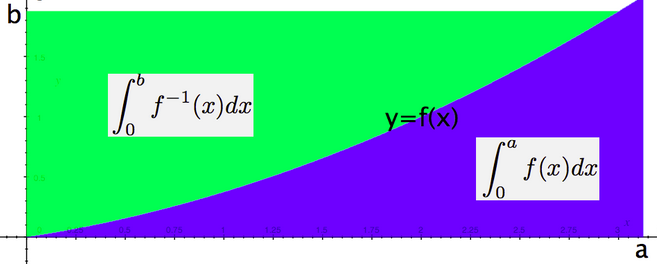
\includegraphics[width=12cm]{intuicao-young} % leia abaixo
\caption{Retirado de \url{https://math.stackexchange.com/questions/149901/geometric-interpretation-of-youngs-inequality}.}
\end{figure}
 

\begin{proposition}[Desigualdade de Holder]
Suponha que $X\in L^p(\Omega)$ e $Y\in L^q(\Omega)$ tal que $p,q\in [1,+\infty]$ e 
$\dfrac{1}{p} +\dfrac{1}{q} = 1.$
Então, 
$$ \|XY\|_1\leq \|X \|_p\|Y\|_q .$$
\end{proposition}

\begin{proof}
O caso em que $p=1$ e $q=\infty$ é trivial. Para $p,q\in(0,+\infty),$ note que, por Young,
\begin{align*}
\E\left(\dfrac{|X|}{\|X\|_p}\dfrac{|Y|}{\|Y\|_q}\right) &\leq  \dfrac{1}{p}\E\left(\dfrac{|X|^p}{\|X\|^p_p}\right)+\dfrac{1}{q}\E\left(\dfrac{|Y|^q}{\|Y\|^q_q}\right)\\
&\leq  \dfrac{1}{p} + \dfrac{1}{q} = 1.
\end{align*}
\end{proof}

\begin{remark}
Note que Cauchy–Schwarz é um caso específico para $q=2.$
\end{remark}


\begin{corollary}
Se $1 \leq p\leq q\leq +\infty$ então $L^q(\Omega)\subset L^p(\Omega).$ 
\end{corollary}
\begin{proof}
Suponha que $X\in L^q(\Omega)$. Se $\alpha = q/p \geq 1$ e $\beta\geq 1$ tal que $1/\alpha+1/\beta = 1$, então por Holder, 
$$\E(|X^p|)=\E(|1\cdot X^p|) \leq (\E(|X^{\alpha\cdot p}|))^{1/\alpha}\cdot (\E(|1|^{\beta}))^{1/\beta} = (\E(|X^q|))^{p/q},$$
ou seja,
$$\|X\|_p \leq \|X\|_q<\infty. $$
\end{proof}












\newpage
\section{Função Geradora de Momento}\label{sec-geradora-momento}


\begin{definition}[Função Geradora de Momento]\index{Função Geradora de Momento}
Seja $X$ uma variável aleatória, definimos a Função Geradora de Momento $M_X$ de $X$ como
$$M_X(t) = \E(e^{Xt}). $$
\end{definition}


\begin{proposition}
Suponha que $????$ , então
$$\dfrac{d }{dt}\E(e^{Xt}) =\E\left(\dfrac{d}{dt}e^Xt\right) =  \E(Xe^{Xt}). $$
\end{proposition}
***terminar a prova


\begin{comment}
\begin{proof}
Vamos usar o TCD, para isso, precisamos limitar
$$\left| \dfrac{e^{X(t+h)}-e^{Xt}}{h}\right| $$
por uma função integrável.

Pelo Teorema do Valor Médio, temos que
$$e^{X(t+h)} - e^{Xt} = Xe^{Xc}h, $$
para algum $t\leq c \leq t+h$, ou seja,
$$\dfrac{e^{X(t+h)} - e^{Xt}}{h} = Xe^{Xc}, $$
\end{proof}
\end{comment}

\begin{example}[Bernoulli]
Seja $X$ Bernoulli com $P(X=1) = p,$ então é fácil ver que
$$M_X(t) = pe^t + 1 - p. $$
\end{example}

\begin{example}[Geométrica]
Seja $X$ geométrica com probabilidade de acerto $p$, então 
\begin{align*}
M_X(t)  &= \sum_{k=1}^\infty e^{tk}(1-p)^{k-1}p\\
		&= \dfrac{e^t p }{1-(1-p)e^t}
\end{align*}
se $(1-p)e^t<1.$
\end{example}

\begin{example}[Binomial] Seja $X$ binomial $B(n,p)$, então
\begin{align*}
M_X(t)  &= \sum_{k=0}^n {n\choose k} e^{tk}(1-p)^{n-k}p^k\\
		&= \sum_{k=0}^n {n\choose k} (1-p)^{n-k}(e^tp)^k = (1-p+  pe^t )^n.
\end{align*}
\end{example}


\begin{example}[Uniforme] Seja $X$ uniforme $U[a,b]$, então
\begin{align*}
M_X(t)  &= \dfrac{1}{b-a}\int_b^a e^{tx} dx =  \dfrac{e^{tb}-e^{ta}}{t(b-a)}.
\end{align*}
\end{example}


\begin{example}[Normal] Seja $X$ normal $N[\mu,\sigma^2]$ e suponha que $\mu=0$ e $\sigma^2=1$, então
\begin{align*}
M_X(t)  &= \dfrac{1}{\sqrt{2\pi}}\int e^{tx} e^{-x^2 / 2} dx \\
	&= \dfrac{e^{t^2 / 2}}{\sqrt{2\pi}}  \int  e^{\-(x-t)^2/2} dx \\
	&= e^{t^2/2}.
\end{align*}
E no caso caso geral, por um simples argumento de mudança de coordenadas, temos que
$$M_X(t) = e^{t\mu + t^2/2\sigma^2}$$
\end{example}



\begin{tcolorbox}
Através da caracterização da F.G.d.M. de uma normal $N(0,\sigma)$, podemos criar a seguinte definição:

\begin{definition}[Sub-Gaussiana]\label{Subgauss}
Seja $X$ uma v.a. centrada. Então $X$ é Sub-Gaussiana com fator de variância $v$ se 
$$M_X(t)\leq e^{ t^2 v/2}. $$
Dizemos que $X\in \mathcal{G}(v).$
\end{definition} 
Isto é, uma  v.a. $X$ centrada é sub-gaussiana se sua função geradora de momento é dominada pela f.g.d.m. de uma v.a. $Y$ normal centrada com variância $v$, isto é, 
$$M_X(t)\leq M_Y(t) .$$ 
\end{tcolorbox}



\newpage
\section{Exercícios Resolvidos}





\begin{xca}[\cite{grimmett2001one}]
Fixada uma sequência $s$ de caras e coroas de tamanho $k$ , prove que com probabilidade 1, eventualmente essa sequência ocorrerá num lançamento de moedas honestas.
\end{xca}
\begin{proof}
Vamos particionar os inteiros positivos em intervalos de tamanho $k$, isto é, 
$$\N = \bigsqcup_{i=0}^\infty A_i,\ A_i = [ik,(i+1)k). $$
Portanto, para qualquer $i\in \N$,
$$\pr(A_i = s) = (1/2)^k. $$
Note que, se $s$ nunca ocorre, em particular $A_i\neq s$, para todo $i\in \N$, e portanto
\begin{align*}
\pr(s\ \text{não ocorrer em $kn$ lançamentos}) &\leq \pr(A_i \neq s,\ i\leq n)\\
& = \prod_i^n \pr(A_i \neq s) \\
& = (1-1/2^k)^n \rarrowlimn 0 .
\end{align*}
Ou seja,
$$\pr(s \text{ ocorrer eventualmente }) = 1. $$
\end{proof}



\begin{xca}[\cite{grimmett2001one}]
Sejam $A_1,\dots,A_n$ eventos com $n\geq 2$, prove que
$$\pr\left( \bigcup^n_{i=1} A_i\right)  = \sum_{i=1}\pr(A_i) -\sum_{i<j}\pr(A_i\cap A_j)  -\sum_{i<j<k}\pr(A_i\cap A_j\cap A_k)-\dots- \pr(A_i\cap\dots\cap A_n). $$
\end{xca}

\begin{proof}
A prova é por indução. Se $n=2$ já sabemos que isso é verdade. Suponha que a afirmação vale para $n$,  vamos mostrar que então vale para $n+1$.

Temos que
\begin{align*}
\pr\left( \bigcup^{n+1}_{i=1} A_i\right) & = \pr\left(A_n \cup  \bigcup^{n}_{i=1} A_i \right)\\
&= \pr(A_n) + \pr(\bigcup^{n}_{i=1} A_i) - \pr(A_n\cap \bigcup^{n}_{i=1} A_i)\\
&= \pr(A_n) + \pr(\bigcup^{n}_{i=1} A_i) - \pr( \bigcup^{n}_{i=1} (A_i\cap A_n)),
\end{align*}
e com isso temos o resultado, via hipótese de indução.
\end{proof}

\begin{xca}[\cite{grimmett2001one}]
Dados eventos $A_1,\dots, A_n$, suponha que é certo que pelo menos um desses eventos, mas não mais que dois, ocorra. Se $\pr(A_i) = p$ e $\pr(A_i\cap A_j)=q,\ i\neq j$, mostre que $p\geq 1/n$ e $q\leq 2/n.$
\end{xca}
\begin{proof}
Pelo exercício anterior,
\begin{align*}
1 = \pr(\bigcup_i^n A_i) &= \sum_i^n\pr(A_i) - \sum_{i<j}\pr(A_i\cap A_j)+0+\dots+0\\
& = np - qn(n-1)/2.
\end{align*}
Então, é fácil ver que
$$1 = np-qn(n-1)/2 \leq np. $$
Além disso,
$$qn(n-1)/2 = np-1 \leq n-1,$$
já que $p\leq 1.$
\end{proof}


\begin{xca}[\cite{grimmett2001one}]
Suponha que $A,B$ são independentes e mostre que $A^c, B$ também são.
\end{xca}
\begin{proof}
Note que
$$\pr(A\cap B) = \pr(A)\pr(B) = (1-\pr(A^c))\pr(B), $$
e isso implica que
$$ \pr(A^c)\pr(B) = \pr(B) - \pr(A\cap B) = \pr(A^c\cap B).$$
\end{proof}



\begin{xca}[Teorema de Waring](\cite{grimmett2001one}) Sejam $A_1,\dots,A_n$ eventos quaisquer e considere $N$ uma v.a. que conta quantos dos $A_i$ ocorreram. Prove que
$$\pr(N = k) = \sum_{i=0}^{n-k}(-1)^i{k+i\choose k}S_{k+i}, $$
onde 
$$S_j = \ds\sum_{i_i<i_2<\dots<i_j}\pr(A_{i_1}\cap\dots\cap A_{i_j} ). $$ 

\end{xca}




\begin{proof}
************************
\end{proof}





\begin{xca}[Desigualdade de Kounias](\cite{grimmett2001one}) Mostre que
$$\pr\left( \bigcup^n_{i=1}A_i \right)\leq \min_k\left\lbrace  \sum_{i=1}^n\pr(A_i) - \sum_{i\neq k} \pr(A_i\cap A_k)  \right\rbrace  .     $$
\end{xca}

\begin{proof}
Já vimos que 
$$\pr\left( \bigcup^n_{i=1} A_i\right)  = \sum_{i=1}\pr(A_i) -\sum_{i<j}\pr(A_i\cap A_j)  -\sum_{i<j<k}\pr(A_i\cap A_j\cap A_k)-\dots- \pr(A_i\cap\dots\cap A_n), $$
e portanto
$$\pr\left( \bigcup^n_{i=1} A_i\right)  \leq \sum_{i=1}\pr(A_i) -\sum_{i<j}\pr(A_i\cap A_j).$$
Agora, considere a matriz $M$ com coordenadas $\pr(A_i\cap A_j)$.  Note que
$$ \sum_{i<j}\pr(A_i\cap A_j) $$
é equivalente a soma das entradas estritamente acima da diagonal de $M$ e que, fixado $k$,
$$\sum_{i\neq k} \pr(A_i\cap A_k)=M_{1,k}+\dots+M_{k-1,k}+M_{k,j+1}\dots+M_{k,n}.$$
Portanto, como cada elemento da expressão acima está estritamente acima da diagonal de $M$,
\begin{align*}
\pr\left( \bigcup^n_{i=1} A_i\right) & \leq \sum_{i=1}\pr(A_i) -\sum_{i<j}\pr(A_i\cap A_j)\\
&\leq\sum_{i=1}\pr(A_i)- \sum_{i\neq k} \pr(A_i\cap A_k) .
\end{align*} 
\end{proof}






\begin{xca}[\cite{spencer-probMethod}]
Sejam $v_1\dots,v_n$ vetores em $\R^n$ tal que $|v_i|=1$ para todo $i.$ Então existem $\sigma_i\in\{+1,-1\}$ tal que 
\begin{align*}
|\sigma_1v_1+\dots\sigma_nv_n|\leq \sqrt{n}
\end{align*}
e da mesma forma, podemos encontrar $\sigma$'s tal que
\begin{align*}
|\sigma_1v_1+\dots\sigma_nv_n|\geq \sqrt{n}.
\end{align*}
\begin{proof}
Considere $\sigma_i$ v.a. uniformes em $\{-1,1\}$ e defina 
$$X = |\sigma_1v_1+\dots\sigma_nv_n|^2 .$$
Note que 
$$\E(X) = \sum_i \sigma_i^2v_i^2 = \sum_i \sigma_i^2 = \sum_i 1 = n .$$
Mas então, deve existir uma configuração de  $\sigma$'s de tal forma que 
$$|\sigma_1v_1+\dots\sigma_nv_n|^2\leq n$$
e uma tal que 
$$|\sigma_1v_1+\dots\sigma_nv_n|^2\geq n.$$
\end{proof}

\end{xca}


Para o próximo exercício, vamos precisar da seguinte definição:

\begin{definition}[Uniformemente Integrável]\index{Uniformemente Integrável}
Seja $H$ uma família de v.a.'s  tal que
$$\sup_{X\in H} \E(|X|)<\infty. $$
Dizemos que $H$ é uma família uniformemente integrável se 
$$\sup_{X\in H} \int_{X>a}|X|d\pr \rightarrow 0,\ a \rightarrow \infty. $$
\end{definition}

\begin{xca}[\cite{chaumont_yor_2012}] 

Dado uma v.a. $X$, considere  a medida limitada
$$ \nu_X(A) = \int_A Xd\pr. $$
Mostre que dado uma família $H$ de v.a.'s não negativas tal que
$$\sup_{X\in H} \E(|X|)<\infty, $$
 então:
\begin{enumerate}
\item $H$ é uniformemente integrável.
\item $\nu_X,\ X\in H$ é equi-absolutamente contínua com respeito à $\pr$, isto é,
$$\forall \e>0,\ \exists \delta>0,\ \forall A\  \textrm{mensurável,}\ \pr(A)\leq \delta \Rightarrow \sup_{X\in H}\nu_X(A)\leq \e. $$
\item Para qualquer sequência  de mensuráveis $(A_n)$ tal que $A_n \downarrow \emptyset$, temos que
$$\lim_{n\rightarrow \infty} \left( \sup_{X\in H} \nu_X(A_n)\right) = 0.$$
\item Para qualquer sequência  disjunta de mensuráveis $(B_n)$, temos que
$$\lim_{n\rightarrow \infty} \left( \sup_{X\in H} \nu_X(B_n)\right) = 0.$$
\end{enumerate}
\end{xca}


\begin{proof}
$ $
\begin{itemize}
\item[1$\rightarrow$2] Suponha que $H$ é uniformemente integrável e tome $\e>0.$ Por hipótese, temos que existe $a'$ grande, tal que
$$\nu_X(X>a')<\e/2,\ \forall X\in H. $$
Agora note que
\begin{align*}
\nu_X(A) &= \nu_X(A\cap(X>a'))+\nu_X(A\cap(X\leq a'))\\
&\leq \nu_X(X>a') + \int_{A\cap (X\leq a')}Xd\pr \\
&\leq  \e/2 + a'\pr(A\cap(X\leq a'))\\
&\leq \e/2 + a'\pr(A).
\end{align*}
Portanto, escolhendo $\delta = \e/(2a')$, temos o resultado.
\item[2$\rightarrow$3] Como $A_n\downarrow \emptyset,$ temos que
$$\lim_n \pr(A_n)=0. $$
Portanto, dado $\e>0$, para todo $n$ suficientemente grande, temos que
$$\pr(A_n)\leq \delta, $$
onde $\delta>0$ é como na hipótese do item 2. Logo,
$$\lim_n (\sup_{X\in H}A_n)\leq \e, $$
e como $\e>0$ é qualquer, temos o resultado.
\item[2$\rightarrow$4] Como
$$\pr(\cup B_n) = \sum \pr(B_n) \leq 1, $$
temos que 
$$\lim_n \pr(B_n) = 0,$$
e isso é suficiente para usarmos o mesmo argumento do item anterior.

\item[4$\rightarrow$3] Suponha que exista uma sequência $(A_n)$ tal que $A_n\downarrow \emptyset$ mas para algum $\e>0$,
$$\lim_{n\rightarrow \infty} \left( \sup_{X\in H} \nu_X(A_n)\right) >\e.$$
Então existe uma subsequência $(X_{n_k},A_{n_k})$ tal que
$$\nu_{X_{n_k}}(A_{n_k})> \e/2. $$
Basta considerar então $B_k = A_{n_k}\backslash A_{n_{k+1}}$, essa sequência é disjunta, mas 
$$\lim_{k\rightarrow \infty} \left( \sup_{X\in H} \nu_X(B_k)\right) >\e/2,$$
contrariando o item  $4.$

\item[3$\rightarrow$1] Suponha que $H$ não é uniformemente integrável. Então, existe $\e>0$ tal que conseguimos uma sequência $(X_{n_k},a_k)$ com $a_k\rightarrow \infty$ tal que
$$\int_{X_{n_k}>a_k}X_{n_k}d\pr >\e/2. $$ 

Tomando 
$$A_k = \bigcup_{i=k}^\infty \{X_{n_k}>a_k\}, $$
conseguimos uma sequência decrescente, tal que
$$\lim_{k\rightarrow \infty} \left( \sup_{X\in H} \nu_X(A_k)\right) >\e/2.$$
Note que isso ainda não é suficiente para chegarmos numa contradição, já que não sabemos se $A_k\downarrow \emptyset.$

Note que podemos supor que $a_k$ é da forma $2^k$, já que se $2^k<a_k$, então
$$\int_{X_{n_k}>2^k} X_{n_k}d\pr \geq  \int_{X_{n_k}>a_k}X_{n_k}d\pr >\e/2. $$

Mas, 
$$\int_{X_{n_k}>2^k} X_{n_k}d\pr > \int_{X_{n_k}>2^k} 2^k d\pr  = 2^k \pr(X_{n_k}>2^k),$$
isto é,
$$\pr(X_{n_k}>2^k) < \dfrac{\sup_{X\in H}\E(X)}{2^k} = \dfrac{C}{2^k}, $$
já que, por hipótese,
$$ \sup_{X\in H}\E(X)<\infty.$$
Temos então que
$$\pr(A_n) = \pr(\bigcup_{i=n}^\infty(X_{n_n} >a_n) )\leq \sum_{i=n}^\infty \dfrac{C}{2^n} \rarrowlimn 0. $$
Isso quer dizer que $A_n \downarrow A$ onde $A$ é um conjunto com medida nula, e portanto mensurável. Logo, considerando uma nova sequência  $A'_n  = A_n\backslash A$, temos o resultado.

\end{itemize}



\end{proof}


\begin{xca}[Distribuição LogNormal não é definida por seus momentos](\cite{chaumont_yor_2012})\index{Distribuição!Lognormal} Seja $N$ uma v.a. com distribuição normal $N(0,\sigma^2).$ Defina
$$X = \exp N. $$
\begin{enumerate}
\item Encontre a densidade de $X$.
\item  Prove que para todo $n,p\in \mathbb{Z}$,
$$\E\left[  X^n \sin \left( \dfrac{p\pi}{\sigma^2}N \right)  \right]=0. $$ 
\item Mostre que existem infinitas probabilidades em $\R_+$ tal que:
\begin{itemize}
\item[i.] Para todo $n\in \mathbb{Z}$,
$$\int x^n d\mu(x) = \exp\left( \dfrac{n^2\sigma^2}{2}\right),   $$
\item[ii. ]$\mu$ tem densidade limitada com respeito à lei de $\exp N.$  
\end{itemize}
\end{enumerate}
\end{xca}

\begin{proof}
$ $
\begin{enumerate}
\item Para $t>0$, temos que
$$\pr(X\leq t) = \pr(\exp N \leq t) = \pr(N\leq \log t), $$
portanto, a densidade de $X$ é dada por
$$\dfrac{d}{dt}\pr(N\leq \log t) = \dfrac{1}{t\sqrt{2\pi \sigma^2}}\exp\left(\dfrac{-(\log t)^2}{ 2\sigma^2}\right)  . $$

\item  Como $$\sin x = \dfrac{e^{ix} - e^{-ix}}{2i}, $$
é fácil ver que 
$$X^n \sin \left( \dfrac{p\pi}{\sigma^2}N\right)  = \textrm{Im}\left(\E(e^{zN}) \right), $$
onde $z = n+\dfrac{\pi p }{\sigma^2} i$. Um simples cálculo nos mostra que
$$\E(e^{zN}) =\exp \left(\dfrac{z^2\sigma^2}{2}\right), $$
já que
$$\exp(zx)\exp\left(-\dfrac{x^2}{2\sigma^2}\right) =\exp\left(-\dfrac{(x-\sigma^2z)^2}{2\sigma^2} \right)\exp \left(\dfrac{z^2\sigma^2}{2}\right).$$


Disso, é fácil ver que, existe uma constante $C>0$ tal que
$$\textrm{Im}\left(\exp \left(\dfrac{z^2\sigma^2}{2}\right)\right) =  C\cdot \sin(np\pi) = 0, $$
já que $n,p\in \mathbb{Z}.$

\item  Seja $f_l(x)$ a função de densidade de $X=\exp N$ que encontramos no item 1.
Pelo item 2, temos que para todo $n\in\mathbb{Z}$,
$$0 = \E(X^n\sin((p\pi/\sigma^2)\log X ))= \int x^n \sin((p\pi/\sigma^2)\log x)f_l(x)dx. $$
Em particular,
$$\int (1+ \sin((p\pi/\sigma^2)\log x))f_l(x)dx =1,$$
ou seja,
$$x\mapsto (1+ \sin((p\pi/\sigma^2)\log x))f_l(x)$$
é uma densidade. De fato, isso é verdade para
$$x\mapsto (1+ \sum_p c_p\sin((p\pi/\sigma^2)\log x))f_l(x),$$
onde $(c_p)$ é uma sequência de números reais tal que $\sum_p |c_p| \leq 1,$ já que
$$1+\sum_p c_p \sin (x)\geq 0.  $$ 
Vamos denotar a lei dada pela densidade acima por $Q_{c_p}.$ Portanto, se $Y$ é distribuída de acordo com $Q_{c_p}$, temos que
\begin{align*}
\E_{Q_{c_p}}(Y^n) &= \int y^n(1+ \sum_p c_p\sin((p\pi/\sigma^2)\log x))f_l(x)dx  \\
& = \int y^n f_l(x)dx\\
& = \E(X^n)\\
& = \E(e^{nN})\\ 
& = \exp\left(\dfrac{n^2\sigma^2}{2} \right).
\end{align*}
Onde a última igualdade vem do item 2.
\end{enumerate}

\begin{tcolorbox}[colback = yellow!60]
Mostramos então que para cada sequência  $(c_p)$, conseguimos uma lei $Q_{c_p}$ tal que se $Y$ tem lei $Q_{c_p}$, então \textbf{todos os momentos}  de $Y$ coincidem com os momentos de $X=e^N$, porém $X$ e $Y$ \textbf{possuem leis diferentes!}. Ou seja, saber os momentos de uma v.a. $Z$ não é suficiente para saber a lei de $Z$.    
\end{tcolorbox}



\end{proof}





















\chapter{Convergência}\label{cap- modos de convergencia}
\begin{tcolorbox}[colback = white]
As Principais referências usadas foram:
\begin{enumerate}
\item \cite{vaart-stat}
\item \cite{durrett}
%\item \cite{shao-statistics}
\end{enumerate}
\end{tcolorbox}

\section{Modos de Convergência}



\begin{definition}\index{Convergência! quase todo ponto}\index{Convergência! em probabilidade} \index{Convergência! em distribuição}
Seja $(X_n)$ uma sequência de vetores aleatórios e $X$ um vetor aleatório.
\begin{enumerate}
\item Dizemos que $X_n$ converge q.t.p. para $X$ se 
$$\pr\left(\lim_{n\rightarrow +\infty} \|X_n-X\| = 0\right) = 1,$$
e simbolizamos tal convergência como $X_n \rightarrow_{qtp}X$.
\item Dizemos que $X_n$ converge para $X$ em probabilidade se  dado $\e>0$,
$$\lim_{n\rightarrow+\infty} \pr(\|X_n-X \|>\e) = 0, $$
e simbolizamos tal convergência como $X_n \rightarrow_{p}X$.

\item Dizemos que $X_n$ converge em $L^p$ para $X$ se, fixado $p>0$,
$$\lim_{n\rightarrow+\infty} \E \|X_n-X\|^p = 0.$$

\item Dizemos que $X_n$ converge para $X$ em distribuição (ou em Lei, ou fracamente) se para cada ponto de continuidade de $x\mapsto \pr(X\leq x)$, temos que
$$ \lim_{n\rightarrow+\infty}  \pr(X_n\leq x) = \pr(X\leq x),$$
e simbolizamos tal convergência como $X_n \rightarrow_{d}X$. 
\end{enumerate}
\end{definition}


\begin{tcolorbox}[colback = yellow!60]
\begin{remark}
Veremos mais adiante que podemos interpretar a convergência em distribuição como uma \textbf{convergência fraca$^*$} no dual das funções contínuas e limitadas (ver Capítulo \ref{} e/ou Teorema \ref{teorema portmanteau} itens 1 e 2, por exemplo). Apesar de se tratar de uma convergência fraca$^*$ e não apenas fraca, por razões histórias abandonamos a $^*$ no nome.
\end{remark}
\end{tcolorbox}








\begin{definition} Seja $(A_n)_{n\in \N}$ uma sequência de eventos mensuráveis. Então
\begin{align*}
\{A_n,\ i.o.\} &= \bigcap_{m=1}^\infty \bigcup_{n=m}^\infty A_n \\
               &= \limsup A_n 
\end{align*}
Observe que
$$\pr(\{A_n,\ i.o.\}) = \lim_{n\rightarrow \infty}\pr\left(\bigcup_{n=m}^\infty A_n\right), $$
já que os conjuntos $B_m = \bigcup_{n=m}^\infty A_n$ são encaixados.
\end{definition}



\begin{tcolorbox}

\begin{lemma}

Seja 
$$B_n^\e = \{\omega\in \Omega:\ \|X_n(\omega)-X(\omega)\|>\e\}, $$
 então, $X_n$ converge para $X$ q.t.p. se, e só se, para todo $\e>0,$
$$\pr(B_n^\e\ i.o.) =0. $$
\end{lemma}
\end{tcolorbox}
\begin{proof}
Dado $\e>0$, se  
$$\pr(B_n^\e\ i.o.) =0, $$
então para quase todo $\omega\in \Omega$, existe $N(\omega,\e)\in \N$ tal que, para $n\geq N(\omega,\e)$,
$$\| X_n(\omega)-X(\omega) \|\leq \e. $$
Mas então, para quase todo $\omega\in \Omega$, temos que
$$\lim_{n\rightarrow +\infty } \| X_n(\omega)-X(\omega) \|\leq \e, $$
e como $\e>0$ é um valor positivo arbitrário, temos que, para quase todo ponto
$$\lim_{n\rightarrow +\infty } \| X_n(\omega)-X(\omega) \|=0, $$
ou equivalentemente,
$$\pr\left(\lim_{n\rightarrow +\infty} \|X_n-X\| = 0\right) = 1.$$

O outro lado é trivial.
\end{proof}

\begin{tcolorbox}[colback = yellow!60]

\begin{remark}
Esta forma de escrever a convergência q.t.p. será útil quando estudarmos os lemas de Borel-Cantelli.

\end{remark}

\end{tcolorbox}


\begin{proposition}
Se $X_n \rightarrow_{\text{q.t.p.}} X$, então $X_n \rightarrow_{\text{p}} X$.
\end{proposition}
\begin{proof}
Se $X_n \rightarrow_{\text{q.t.p.}} X$, então dado $\e>0$ já vimos que
$$\pr(\|X_n-X\|> \e,\ i.o.)  = 0. $$ Mas então
\begin{align*}
\lim_{n\rightarrow\infty}\pr(\|X_n-X\|> \e) &\leq \lim_{n\rightarrow\infty} \pr\left(\bigcup_{i=n}^\infty\|X_n-X\|> \e\right)\\
&= \pr(\|X_n-X\|>\e,\ i.o.) = 0.
\end{align*}
\end{proof}

\begin{proposition}
Se $X_n \rightarrow_{\text{p}} X$, então $X_n \rightarrow_{d} X$.
\end{proposition}

\begin{proof}
Dado $\e>0$,
\begin{align*}
\pr(X_n\leq x) & = \pr(X_n\leq x,\ X\leq x+\e) + \pr(X_n\leq x,\ X> x+\e)\\
&\leq \pr(X\leq x+\e) + \pr(\|X_n-X\|>\e).
\end{align*}
E da mesma forma
\begin{align*}
\pr(X\leq x-\e) & = \pr(X_n\leq x,\ X\leq x-\e) + \pr(X_n> x,\ X\leq x+\e)\\
&\leq \pr(X_n\leq x) + \pr(\|X_n-X\|>\e).
\end{align*}
E portanto, temos que
$$\ds\pr(X\leq x-\e) -  \lim_n\pr(\|X_n-X\|>\e)\leq \ds \liminf_n\pr(X_n\leq x),$$
e também
$$  \ds \limsup_n \pr(X_n\leq x)\leq \ds\pr(X\leq x+\e)+ \lim_n\pr(\|X_n-X\|>\e).$$
Ou seja, 
$$ \pr(X\leq x-\e)\leq\liminf_n\pr(X_n\leq x)\leq \limsup_n \pr(X_n\leq x)\leq \ds\pr(X\leq x+\e),$$
já que a sequência converge em probabilidade.
Como estamos supondo que $F_X(x) = \pr(X\leq x)$ é contínua em $x$ e que $\e>$ é qualquer, temos o resultado.
\end{proof}

\begin{tcolorbox}[colback = yellow!60]
\begin{remark}
Temos então que 
$$(\textrm{q.t.p.}) \Rightarrow (\textrm{probabilidade}) \Rightarrow (\textrm{distribuição}) $$
\end{remark}
\end{tcolorbox}

\newpage
\section{Convergência Fraca em $\mathbb{R}^k$}

\subsection{Teorema Portmanteau}
\begin{tcolorbox}
\begin{theorem}[Portmanteau]\label{teorema portmanteau}\index{Teorema! Portmanteau}\footnote{Portmanteau significa maleta em francês.} Para qualquer sequência $(X_n)$ de vetores aleatórios e $X$ um vetor aleatório, são equivalentes:
\begin{enumerate}
\item $X_n \rightarrow_{\textrm{d}} X$
\item $\E(f(X_n))\rightarrow \E(f(X))$ para toda $f$ contínua e limitada.
\item $\E(f(X_n))\rightarrow \E(f(X))$ para toda $f$ Lipschitz e limitada.
\item $\liminf_n \E(f(X_n))\geq \E(f(X))$ para toda  $f$ contínua  e não negativa.
\item $\liminf_n \pr(X_n\in G)\geq \pr(X\in G)$ para todo $G$ aberto.
\item $\limsup_n \pr(X_n\in F)\leq \pr(X\in F)$ para todo $F$ fechado.
\item $\pr(X_n\in B)\rarrowlimn \pr(X\in B)$ para todo Boreliano $B$ tal que $\pr(X\in \delta B)=0$. 
\end{enumerate}
\end{theorem}
\end{tcolorbox}



\begin{proof}[Demonstração do Teorema Portmanteau]
$ $

Vamos seguir a demonstração de \cite{vaart-stat}.

\textrm{1$\rightarrow$ 2:}
Vamos supor que $F_X(x)= \pr(X\leq x)$ é  contínua para todo $x$.
Utilizando a hipótese, temos que, para qualquer retângulo fechado $I\subset \R^d$,
$$\pr(X_n\in I) \rarrowlimn \pr(X\in I). $$
Podemos escolher um retângulo $I$ grande o suficiente de tal forma que
$$\pr(X\not\in I)< \e, $$
já que $\pr(X\in \R^m) = 1$.

Como $f$ é contínua e portanto absolutamente contínua em $I$ (já que este é compacto), podemos particionar $I$ em uma quantidade finita retângulos menores $I_j$, com $j=1,2,\dots,k$ de tal forma que para todo $0\leq j\leq k$,
$$|f(x)-f(y)|< \e,\ x,y\in I_j .$$
Fixado um ponto $x_j\in I_j$ para cada $I_j$, defina 
$$f_\e = \sum_j f(x_j)1_{Ij}. $$ 
Sem perda de generalidade, podemos supor que $f\in [-1,1]$, já que $f$ é limitada, e portanto
\begin{align*}
|\E(f(X_n))-\E(f_\e(X_n))  | & = |\E([f(X_n)-f_\e(X_n)]1_{X_n\in I})+|\E([f(X_n)-f_\e(X_n)]1_{X_n\not\in I}) \\
& \leq \e + 2\pr(X_n\not\in I),
\end{align*}
e então, para $n$ grande o suficiente, temos que 
$$|\E(f(X_n))-\E(f_\e(X_n))  |< 3\e. $$
E o mesmo vale para $X$, isto é,
\begin{align*}
|\E(f(X))-\E(f_\e(X))  | & \leq \e + 2\pr(X\not\in I) \leq 3\e.
\end{align*}
Por fim, temos que
\begin{align*}
|\E(f(X))-\E(f(X_n))| & = |\E(f(X))-\E(f(X_n)) \pm \E(f_\e(X)) \pm\E(f_\e(X_n))|\\
&\leq |\E(f(X))-\E(f_\e(X))|&\\
& + |\E(f(X_n))-\E(f_\e(X_n))| \\
& + |\E(f_\e(X))-\E(f_\e(X_n))|, 
\end{align*}
portanto, só precisamos controlar o último termo. Mas note que
\begin{align*}
|\E(f_\e(X))-\E(f_\e(X_n))| &\leq \sum_j |\pr(X_n\in I_j)-\pr(X\in I_j)||f(x_j)| \rarrowlimn 0.
\end{align*} 
Para a demonstração  no caso geral, recomendamos a leitura da Seção \ref{section- distribuicoes} para melhor entendimento da função de distribuição e depois do item (a) do Teorema 2.2 em  \cite{vaart-stat}.

\textrm{2$\rightarrow$ 3:} Óbvio.

\textrm{3$\rightarrow$ 5:} Note que
$$f_m(x) = (m\cdot \textrm{dist}(x,G^c))\wedge 1 $$
é Lipschitz, limitada e 
$$f_m(x)\uparrow 1_{G}(x) ,$$
portanto, como
$$f_m(x)\leq 1_{ G}(x),  $$
temos que, \emph{por hipótese},
$$ \liminf_n \pr(X_n\in G) \geq \liminf_n \E(f_m(X_n)) = \E(f_m(X)),$$
e pelo teorema da convergência monótona,
$$\lim_m  \E(f_m(X)) =  \E(1_G(X)) = \pr(X\in G).$$

\textrm{5$\leftrightarrow$ 6:} Basta tomar o complementar.

\textrm{5+6$\rightarrow$ 7:} Lembre-se que $\delta B =\overline{B}- B^\circ$. Então por (5) e (6), temos que
$$ \pr(X\in \overline{B})\geq \limsup \pr(X_n\in \overline{B})\geq \liminf \pr(X_n\in B^\circ)\geq \pr(X\in B^\circ). $$
Como $\pr(\delta B) = 0$, temos que $\pr(X\in \overline{B}) = \pr(X\in B^\circ)$ e portanto, provamos o que queríamos, já que $\pr(X\in B)\leq \pr(X\in \overline{B})$ e $\lim_n\pr(X_n\in B)$ está entre os $\limsup$ e $\liminf$ acima. 


\textrm{7$\rightarrow$1:} Se $F_x$ é contínua em $x$, então 
$$\pr(X= x )=\pr\left(X\in \delta \left(\prod^d(-\infty,x]\right) \right)=0. $$ 

\textrm{2$\rightarrow$4:} Tome $f$ contínua, não negativa e defina
$$f_m = f\cdot 1_{f\leq m}.$$
Note que $0\leq f_m\uparrow f$ e $f_m$ é contínua e limitada. Logo, por hipótese,
\begin{align*}
\liminf_n \E(f(X_n)) &\geq \liminf_n \E(f_m(X_n)) = \E(f_m(X)).
\end{align*}
Por fim, utilizando o teorema da convergência monótona, temos que
\begin{align*}
\liminf_n \E(f(X_n))= \lim_m\liminf_n \E(f(X_n)) &\geq \lim_m \E(f_m(X)) = \E(f(X)).
\end{align*}


\textrm{4$\rightarrow$2:} Suponha inicialmente que $f$ é continua, não negativa e que $f\leq M$. Por hipótese, temos que
$$\liminf \E(f(X_n)) \geq \E(f(X)).$$
Como $0\leq M-f$, também por hipótese, temos que
$$
\begin{array}{lll}
\liminf \E(M-f(X_n)) &\geq \E(M-f(X)),
\end{array}
$$
isto é,
$$\E(f(X)) \geq  \limsup \E(f(X_n)), $$
e portanto
$$\liminf \E(f(X_n))\geq \E(f(X)) \geq  \limsup \E(f(X_n)).$$
concluindo o resultado.

No caso geral, basta escrever $f$ como
$$f= f^+ - f^-,$$
com $f^+\geq 0,$ e $f^-\geq 0$ e concluímos o teorema.
\end{proof}



\begin{tcolorbox}[colback = yellow!60]
\begin{remark}[Como lembrar de Portmanteau] Uma forma de lembrar da direção das inclusões nos itens (5) e (6) é considerando o caso em que $\pr(X_n = x_n) = 1$. Para isso, suponha que $G$ é aberto, que $(x_n)\subset G$ e que $x_n\rarrowlimn x\in \delta G = \overline{G} -  G^\circ$, então $X_n \rightarrow_d X$, onde $\pr(X=x)=1$, e daí
$$1 = \liminf_n \pr(X_n\in G)\geq \pr(X\in G) = 0. $$

Da mesma forma, tomando o fechado $F= G^c$, temos que
$$0 = \limsup_n \pr(X_n\in G^c)\leq \pr(X\in G^c) = 1. $$
\end{remark}
\end{tcolorbox}



\begin{tcolorbox}[colback = yellow!60]
\begin{remark}\label{obs-portmanteu-tight}
Note que se $B[0;M]$ é a bola fechada de raio $M$ centrada na origem, então
$$\{\|X\|>M\} = \{X\in B[0;M]^c\}. $$
Primeiramente note que, como $B[0;M]$ é fechado, então $B[0;M]^c$ é aberto, então se $X_n \rightarrow_d X$, pelo Teorema \ref{teorema portmanteau}, temos que
\begin{align*}
 \liminf \pr(X_n\in B[0;M]^c)&\geq \pr(X\in B[0;M]^c), 
\end{align*}
ou seja,
\begin{align*}
 \liminf \pr(\|X_n\|>M)&\geq \pr(\|X\|>M).
\end{align*}
Da mesma forma, se considerarmos,
$$\{\|X\|\geq M\} = \{X\in B(0;M)^c\}, $$
onde $B(0;M)$ é a bola aberta de raio $M$ centrada na origem, temos que $B(0;M)^c$ é fechado e portanto se $X_n \rightarrow_d X$,
\begin{align*}
 \limsup \pr(\|X_n\|\geq M)&\leq \pr(\|X\|\geq M).
\end{align*}
\end{remark}
\end{tcolorbox}

A proposição a seguir nos mostrar o poder do Teorema Portmanteau \ref{teorema portmanteau}.


\begin{tcolorbox}
\begin{proposition}[Algumas consequências de Portmanteau]\label{prop - conseq-portmnt} Sejam $(X_n)$ e $(Y_n)$ dois vetores aleatórios e $c$ uma constante, então
\begin{enumerate}
\item  $X_n \rightarrow_p c$ se, e só se, $X_n \rightarrow_d c$.

\item  Se $X_n \rightarrow_d X$ e $d(X_n,Y_n) \rightarrow_p 0 $, então $Y_n \rightarrow_d X$.

\item  Se $X_n \rightarrow_d X$ e $Y_n \rightarrow_p c $, então $(X_n,Y_n)\rightarrow_d (X,c).$

\item  Se $X_n \rightarrow_p X$ e $Y_n \rightarrow_p Y $, então $(X_n,Y_n)\rightarrow_p (X,Y).$
\end{enumerate}

\end{proposition}


\end{tcolorbox}
\begin{proof}
$ $
\begin{enumerate}

\item A ida é óbvia já que  (probabilidade)$\Rightarrow$(distribuição). Agora suponha que $X_n \rightarrow_d c.$ Por \ref{teorema portmanteau}, temos que
\begin{align*}
\limsup_n \pr(\|X_n-c\| \geq  \e) &= \limsup_n  \pr(X_n \in B(c,\e)^c)
& \leq \pr(c\in B(c,\e)^c) = 0
\end{align*}

\item Considere uma função $f$ Lipschitz e limitada. Podemos supor sem perda de generalidade que a constante de Lipschitz de $f$ é igual a $1$ e que $f\in[0,1]$.
Temos então que
\begin{align*}
|\E(f(X_n)) - \E(f(Y_n))| & \leq \E|f(X_n) -f(Y_n)|\\
&  = \E|f(X_n) -f(Y_n)|1_{d(X_n,Y_n)\leq\e}\\
& +\E|f(X_n) -f(Y_n)|1_{d(X_n,Y_n)>\e}\\
& \leq \e \pr(d(X_n,Y_n)\leq \e) + 2 \pr(d(X_n,Y_n)> \e)\\
&\leq \e +  2 \pr(d(X_n,Y_n)> \e).
\end{align*}
Note que, $ \pr(d(X_n,Y_n)> \e) \rarrowlimn 0$ por hipótese, e como $\e>0$ é qualquer,
$$|\E(f(X_n)) - \E(f(Y_n))| \rarrowlimn 0, $$
isto é, as sequências $\E(f(X_n))$ e $\E(f(Y_n))$ tem o mesmo limite, porém, sabemos que
$$\E(f(X_n)) \rarrowlimn \E(f(X)), $$
pelo item 3 de \ref{teorema portmanteau}. Portanto, mostramos que que para qualquer $f$ Lipschitz e limitada,
 $$\E(f(Y_n)) \rarrowlimn \E(f(X)), $$
o que é equivalente por \ref{teorema portmanteau} a $Y_n \rightarrow_d X$.


\item Note que
$$d( (X_n,Y_n),(X_n,c)) = d(Y_n,c) \rarrowlimn 0, $$
logo, pelo item anterior, basta mostrarmos que
$$(X_n,c)\rightarrow_d (X,c). $$
Note que dada qualquer 
$$f:(x,y)\mapsto f((x,y))$$ contínua e limitada, temos que
$$f_c:x\mapsto f(x,c),$$
 é contínua e limitada. Como $X_n \rightarrow_d X$, temos que
 $$\E(f(X_n,c)) = \E(f_c(X_n)) \rarrowlimn \E(f_c(X))= \E(f(X,c)). $$
Como $f$ era qualquer função contínua e limitada, temos o resultado por \ref{teorema portmanteau}.


\item Basta notar que
\begin{align*}
d((X_n,Y_n),(X,Y)) &= \sqrt{((X_n-X)^2 + (Y_n-Y)^2 )}\\
&  \leq d(X_n,X) + d(Y_n,Y).  
\end{align*}

\end{enumerate}
\end{proof}





\begin{tcolorbox}
\begin{theorem}[Teorema da Aplicação Contínua]\index{Teorema! Aplicação Contínua}\label{teorema aplicacao continua} Seja $f:\R^k\rightarrow \R^m$ uma função contínua e mensurável em quase todo ponto. Então
\begin{enumerate}
\item Se $X_n\rightarrow_{\textrm{q.t.p.}} X$ então $f(X_n)\rightarrow_{\textrm{q.t.p.}} f(X)$.
\item Se $X_n\rightarrow_{\textrm{p}} X$ então $f(X_n)\rightarrow_{\textrm{p}} f(X)$.
\item Se $X_n\rightarrow_{\textrm{d}} X$ então $f(X_n)\rightarrow_{\textrm{d}} f(X)$.
\end{enumerate}
\end{theorem}
\end{tcolorbox}

\begin{proof}
$ $
\begin{enumerate}
\item É óbvio da definição de convergência q.t.p. e do fato de $g$ ser contínua.
\item Fixe $\e>0$. Dado $\delta>0$, defina $B_\delta$ como o conjunto formado por todos os pontos $x$ tal que \textbf{existe} $y$ satisfazendo
$$(\|x-y\|< \delta ) \ \wedge \  ( \|f(x)-f(y)  \| > \e ). $$
Dado $\omega\in \Omega$, suponha que $\|f(X(\omega))-f(X_n(\omega))\|> \e.$ Então, ou 
$$\|X(\omega)-X_n(\omega)\|< \delta$$
 e portanto
$$X(\omega)\in B_\delta,$$
ou então 
$$\|X(\omega)-X_n(\omega)\|\geq  \delta.$$
Temos então que
$$\pr(\omega:\|f(X(\omega))-f(X_n(\omega))\|>\e)\leq \underbrace{\pr(\omega:X(\omega)\in B_\delta)}_{\textrm{I}} + \underbrace{\pr(\omega:\|X_n(\omega)-X(\omega)\|\geq \delta)}_{\textrm{II}}. $$
Note que o termo II na expressão acima tende a zero, para qualquer $\delta>0$, quando $n$ cresce, já que por hipótese temos convergência em probabilidade.
Além disso, note que os conjuntos $B_\delta$ são encaixados quando diminuímos $\delta$, e que, a menos de um conjunto de medida nula,
$$ \bigcap_{\delta \rightarrow 0} B_\delta  = \emptyset.$$
já que $g$ é continua. Portanto,
$$\pr(\omega:X(\omega)\in \bigcap_\delta B_\delta) = \lim_{\delta \rightarrow 0}\pr(\omega:X(\omega)\in B_\delta) = 0. $$
Como $\delta>0$ foi escolhido qualquer, temos o resultado.

\item  Vamos usar o item 6 do Teorema \ref{teorema portmanteau}, para provar que
$$f(X_n)\rightarrow_d f(X). $$
É claro que 
$$\{ f(X_n)\in F \} = \{X_n \in f^{-1}(F) \}. $$
Além disso, se $F$ é \emph{fechado qualquer}, e $C$ é o conjunto de medida total tal que $f$ é contínua para todo ponto em $C$, temos que
$$f^{-1}(F)\subset \overline{f^{-1}(F)}\subset f^{-1}(F)\cup C^c. $$
A segunda inclusão é facilmente provada, usando o fato de que $f$ é contínua. Por \ref{teorema portmanteau}, usando o fato de que $X_n \rightarrow_d X$,
\begin{align*}
\limsup_n \pr(f(X_n)\in F) & = \limsup_n \pr(X_n\in f^{-1}(F))\\
&\leq \limsup_n \pr(X_n\in \overline{f^{-1}(F)})\\
&\leq \pr(X\in \overline{f^{-1}(F)})\\
&\leq  \pr(X\in f^{-1}(F)\cup C^c)\\
&\leq  \pr(X\in f^{-1}(F))+0\\
&\leq  \pr(f(X)\in F).
\end{align*}
Como $F$ é qualquer fechado, pelas equivalências do Teorema \ref{teorema portmanteau}, temos o resultado.

\end{enumerate}
\end{proof}





\begin{comment}

\begin{definition}[Uniformemente Tight]\index{Tight} Dizemos que uma família $\{X_\alpha:\alpha\in A\}$ é uniformemente tight se para todo $\e>0$, existe $M>0$ tal que
$$\sup_\alpha \pr(\|X_\alpha\|>M) < \e. $$
\end{definition}

\begin{tcolorbox}[colback = yellow!60]
\begin{remark}
Como 
$$\{\|X\|>M\} = \{X\in B[0;M]^c\}, $$
se $(X_\alpha)$ é uniformemente tight, podemos pensar que existe um compacto grande ($B[0;M]$) tal que $(X_\alpha)$ está contida nesse compacto com probabilidade $1-\e$.
\end{remark}
\end{tcolorbox}




\begin{definition}[Quase Função de Distribuição] Uma função $F$ é  quase uma função de distribuição  se ela satisfaz as propriedades das funções de distribuição porém, pode acontecer que 
$$\lim_{n\rightarrow +\infty} F(x)<1,$$ 
e/ou 
$$\lim_{n\rightarrow -\infty} F(x)>0.$$ 

\end{definition}





\begin{tcolorbox}
\begin{theorem}[Lema de Helly] Seja $(F_n)$ uma sequência de funções de distribuição em $\R^k$, então existe uma subsequência $n(k)$ tal que
$$F_{n(k)}(x) \rightarrow F_(x)$$
para cara ponto de continuidade de uma quase função de distribuição $F$.
\end{theorem}
\end{tcolorbox}


\begin{tcolorbox}

\begin{theorem}[Teorema de Prohorov]\index{Teorema! Prohorov} \label{teorema-prohorov} Seja $(X_n)$ uma sequência de vetores aleatórios em $\R^k$. Então
\begin{enumerate}
\item Se $X_n \rightarrow_d X$, então $(X_n)$ é uniformemente tight.
\item Se $(X_n)$ é uniformemente tight, então existe uma subsequência $n(k)$ tal que
$X_{n(k)} \rightarrow_d X$, para algum $X$.
\end{enumerate}

\end{theorem}
\end{tcolorbox}


\begin{proof} Temos que:
\begin{enumerate}

\item Como $X_n \rightarrow_d X$, pelo Teorema \ref{teorema portmanteau}, temos que, dado $\e>0$, para $M$ suficientemente grande
$$ \limsup_n \pr( \|X_n\| \geq M )\leq \pr(\|X\|\geq M)< \e,  $$
ou seja, existe $N$ tal que se $n> N$, então
$$ \pr(\|X_n\|> M)\leq \pr(\|X_n\|\geq  M)< \e.$$ 
Agora, para cada $i\in {1,2,\dots,N}$, existe $M_i$ tal que
$$\pr(\|X_i\|> M_i)\leq \e, $$
tomando $\tilde{M}$ como o máximo entre todos esses valores de  $M$, temos o resultado.


\item  

\end{enumerate}
\end{proof}



\end{comment}



\begin{tcolorbox}

\begin{theorem}[Slutsky]\label{teorema-slutsky}\index{Teorema!Slutsky} Sejam $X_n,\ Y_n,\ X$ vetores aleatórios (ou v.a.'s possivelmente). Se $X_n \rightarrow_d X$ e $Y_n\rightarrow_d c$, para uma constante $c$, então
\begin{enumerate}
\item $X_n+Y_n \rightarrow_d X+c$
\item $Y_n X_n \rightarrow_d c\cdot X$
\item $Y_n^{-1}X_n \rightarrow_d c^{-1}\cdot X$, se $c\neq 0.$

\end{enumerate} 

\end{theorem}

\end{tcolorbox}


\begin{proof}
Pela Proposição \ref{prop - conseq-portmnt}, temos que $Y_n \rightarrow_p c,$ e com isso, também temos que 
$$(X_n,Y_n) \rightarrow_d (X,c). $$

Como, $(x,y)\mapsto x+  y$ e   $(x,y)\mapsto x\cdot y$ são aplicações contínuas, por \ref{teorema aplicacao continua}, temos que o resultado. 
\end{proof}

\begin{definition}[Distribuição Defeituosa]\label{def-distdefeituosa}\index{Distribuição! Defeituosa}
Uma Função de Distribuição Defeituosa é uma função que satisfaz todas as propriedades de funções de distribuição, porém seu limite em $+\infty$ pode ser menor que 1 e seu limite em $-\infty$ pode ser maior que 0.

********melhorar isso no futuro
\end{definition}

\subsection{Teorema de Prohorov}

\begin{tcolorbox}
\begin{theorem}[Teorema de Seleção de Helly]\label{teo- helly}\index{Teorema! Seleção de Helly}\index{Helly} Toda sequência $(F_n)$ de distribuições em $\R^k$ possui uma subsequência $F_{n_k}$ tal que 
$$F_{n_k}(x) \rightarrow F(x),\ k\rightarrow \infty $$
para cada ponto de continuidade de uma função de  distribuição $F$, possivelmente   defeituosa.
\end{theorem}
\end{tcolorbox}
\begin{proof}
Seja considere uma enumeração $\{q_1,q_2,\dots\}$ de $\mathbb{Q}^k$. 
Para um $j$ fixado, note que
$$(F_n(q_i))_n\subset [0,1],$$
e portanto conseguimos uma subsequência de $(F_n(q_i))_n$ convergindo para um limite que vamos chamar de $G(q_1)$. Por um simples argumento de diagonalização, conseguimos uma subsequência $(F_{n_k})$, tal que, para todo $q_j$, temos que
$$F_{n_l}(q_j) \rightarrow G(q_j),\ l\rightarrow \infty. $$
Defina
$$F(x) = \inf \{ G(q): q\in \mathbb{Q},\ q>x\}.  $$
Como para cada $n$, $F_n$ é não decrescente, temos que se $q_j\leq q_l$, então 
$$G(q_j)\leq G(q_l), $$
e daí é fácil ver que $F$ é não decrescente.
\bigskip
\begin{claim}
$F$ é contínua à direita.
\end{claim}
\begin{claimproof}
Note que 
\begin{align*}
\lim_{x_n\downarrow x} F(x_n) &= \inf\{ G(q): q\in \mathbb{Q},\ q>x_n,\ \textrm{para algum}\ n\}\\
&= \inf\{ G(q): \ q>x,\  q\in \mathbb{Q}\} = F(x).
\end{align*}
\end{claimproof}
\bigskip
\begin{claim}
$(F_{n_k})$ converge pontualmente em pontos de continuidade de $F$
\end{claim}
\begin{claimproof}
Seja $x$ um ponto de continuidade de $F$. Dado $\e>0$, tome $a<b<x<c$ pontos racionais próximos o suficiente de $x$ tal que
$$F(x)-\e < F(a)\leq F(b)\leq F(x)\leq F(c)< F(x)+\e .$$
Sabemos que
$$F_{n_k}(b)\leq F_{n_k}(x)\leq F_{n_k}(c), $$
já que cada $F_n$ é uma distribuição. Agora note que
$$F_{n_k}(b) \rightarrow G(b) \geq F(a),$$
já que $a<b$. Além disso,  para todo $q>c$, sabemos que
$$ G(c)\leq G(q),$$
isto é,
$$G(c)\leq \inf_{q>c}G(q)  = F(c), $$
e portanto
$$f_{n_k}(c)\rightarrow G(c)\leq F(c). $$
Mas então, tomando $k$ suficientemente grande, as observações anteriores nos dizem que
$$ F(x)-\e <F(a)\leq F_{n_k}(b)\leq F_{n_k}(x)\leq F_{n_k}(c)\leq F(c)\leq F(x)+\e,  $$
ou seja,
$$|F(x)-F_{n_k}(x)|<\e $$
e como $\e>$ foi qualquer, temos o resultado.
\end{claimproof}


Note que o que fizemos até então é suficiente para provar o Teorema no caso em que $k=1$, já que o fato de $F$ ser não decrescente é suficiente para garantir que
$$\mu((a,b]) = F(b)-F(a)\geq 0, $$
e então conseguimos induzir uma medida finita no nosso espaço.

Porém, no caso em que $k>1$ temos um trabalho extra de provar que da fato $F$ atribui valores não negativos nos respectivos cubos $k$-dimensionais (equivalentes aos intervalos em $\R$). Faremos o resto da prova em uma versão futura destas notas, apesar do argumento ser bem simples.

\end{proof}


\begin{definition}[Família Tight]\label{def - tight} \index{Tight}  Uma família $\{X_\alpha:\alpha\in A\}$ é \textbf{tight} se para todo $\e>0$, existe $M>0 $ tal que 
$$\sup_\alpha \pr(\|X_\alpha\|>M)<\e. $$
\end{definition}
\begin{tcolorbox}[colback = yellow!60] Isto é, uma família de vetores aleatórios é tight, se existe um compacto grande o suficiente de tal forma que esta família está suportada neste compacto com probabilidade alta.
\end{tcolorbox}






\begin{theorem}[Teorema de Prohorov]\label{teo - prohorov} \index{Teorema! Prohorov}\index{Prohorov} Seja $(X_n)$ uma sequência de vetores aleatórios em $\R^k$.  Então
\begin{enumerate}
\item Se $X_n \rightarrow_d X$ para algum $X$,  então $(X_n)$ é tight.
\item Se $(X_n)$ é tight, então existe uma subsequência $(X_{n_k})$ tal que 
$$X_{n_k}\rightarrow_d X$$
para algum $X.$ 
\end{enumerate}
\end{theorem}
\begin{proof}
$ $
\begin{enumerate}
\item Tome $M$ grande o suficiente para que
$$\pr(\|X\|\geq M)< \e. $$
Por Portanteau \ref{teorema portmanteau} (ou Observação \ref{obs-portmanteu-tight}), temos que
$$\limsup_n \pr(\|X_n\|\geq M)\leq \pr(\|X\|\geq M)<\e. $$
Portanto,  para $N$ grande, se $n\geq N$, 
$$ \pr(\|X_n\|\geq M)\leq \e. $$
Para lidar com os índices menores que $N$, basta considerar $M$ um pouco maior, se necessário.

\item Seja $F_n$ a função de distribuição de $X_n$. Pelo Teorema de Seleção de Helly \ref{teo- helly}, conseguimos uma subsequência $(F_{n_k})$ que converge para uma função de distribuição  $F$,  possivelmente defeituosa. 

Como $(X_n)$ é tight, dado $\e_i = 1/i$ com $i= 1,2\dots$, existe $M_i$ tal que, para todo $n\in \N$
$$\pr(\|X_n\|\leq M_i)>1-\e_i. $$
É claro que isso implica que, para todo $n\in \N$
$$F_n(M) = \pr(X_n \leq M_i)>1-\e_i, $$
já que
$$\{\|X_n\|\leq M_i\}\subset \{X_n \leq M_i\}. $$
Fazendo $M_i$ um pouco maior, se necessário, podemos supor que $M_i$ é um ponto de continuidade de $F$, e portanto
$$F(M_i) = \lim_kF_{n_k}(M_i)\geq 1-1/i.  $$
Logo, se $x\rightarrow +\infty$, basta tomar uma sequência $(M_{i_j})$ com  $x\geq M_{i_j}$ e $M_{i_j} \rightarrow +\infty$ e  então temos que $F(x)\rightarrow 1$.

O argumento para quando $x\rightarrow -\infty$ é semelhante. (faça um desenho)

\end{enumerate}
\end{proof}







\newpage
\section{Exercícios Resolvidos}







\chapter{Teorema Central do Limite }

\begin{tcolorbox}[colback = white]
As Principais referências usadas foram:
\begin{enumerate}
\item \cite{durrett}.
\item \cite{stroock}.
\end{enumerate}
\end{tcolorbox}



\section{Motivação: Teorema de De Moivre-Laplace }

Seja $X_1,\dots,X_n$ uma sequência de v.a.'s i.i.d. com $\pr(X=1)= \pr(X=-1)=1/2$ e considere $S_n = X_1+\dots+X_n.$ Note que
$$\pr(S_{2n} = 2k) = {2n\choose n+k}2^{-2n},$$
já que para $S_{2n}=2k$, precisamos que $1\cdot(2n + A) -1\cdot(2n+B) =2k$ e que
$(2n+A)+(2n+B)= 2n$. Por Stirling \ref{sec-stirling}, não é difícil mostrar que


\begin{align*}
{2n\choose n+k}2^{-2n} &\sim \left( 1+\dfrac{k}{n} \right)^{-n-k}\left( 1-\dfrac{k}{n} \right)^{-n+k}\left( 1+\dfrac{k}{n} \right)^{-1/2}\left( 1-\dfrac{k}{n} \right)^{-1/2}(\pi n)^{-1/2}.
\end{align*}
Além disso,
$$ \left( 1+\dfrac{k}{n} \right)^{-n-k}\left( 1-\dfrac{k}{n} \right)^{-n+k} =  \left( 1-\dfrac{k^2}{n^2} \right)^{-n}\left( 1+\dfrac{k}{n} \right)^{-k}\left( 1-\dfrac{k}{n} \right)^{k}.$$

\begin{lemma}\label{lema-limitefundamental-convergenciaparaexponencial}
Suponha que $a_i \rightarrow +\infty $, que $c_i\rightarrow 0 $ e $a_ic_i \rightarrow \lambda$, então
$$\left( 1 + c_i \right)^{a_i} \rightarrow e^{\lambda}. $$
\end{lemma}
\begin{proof}
Vamos usar a identidade 
$$\dfrac{\log(1+x)}{x}\rightarrow 1,\ x\rightarrow 0. $$
Temos então que
\begin{align*}
\dfrac{\log(1+c_j)}{c_j} &=\dfrac{a_j}{a_j}\dfrac{\log(1+c_j)}{c_j} \rightarrow 1,
\end{align*}
ou seja,
\begin{align*}
a_j\log(1+c_j)= \lim_ja_jc_j =\lambda.
\end{align*}
Tomando $\exp$ dos dois lados, temos o resultado.
\end{proof}
\begin{lemma}\label{lema-limitefundamental-convergenciaparaexponencial-GENERALIZADA}
Suponha que 
\begin{enumerate}
\item $\ds\max_{1\leq j\leq n}|c_{j,n}|\rarrowlimn 0$,
\item $\ds\sum^{n}_{j=1}c_{j,n} \rarrowlimn \lambda$,
\item $\ds \sup_n \ds\sum^n_{j=1}c_{j,n}<\infty.$
\end{enumerate}
Então,
$$\prod^n_{j=1}(1+c_{j,n})\rightarrow e^\lambda. $$
\end{lemma}

\begin{proof}
Por 1, $${\log(1+c_{j,n})}\sim {c_{j,n}}.$$
Por 3,
$$\dfrac{\sum_{j=1}^n \log(1+c_{j,n})}{\sum_{j=1}^n c_{j,n}}\sim 1. $$
E então, por 2
$$\sum_{j=1}^n c_{j,n}\dfrac{\sum_{j=1}^n \log(1+c_{j,n})}{\sum_{j=1}^n c_{j,n}}\sim \sum_{j=1}^n c_{j,n}\sim \lambda. $$
E daí basta aplicar a exponencial dos dois lados.

\end{proof}









Utilizando o lema \ref{lema-limitefundamental-convergenciaparaexponencial}, se considerarmos $x = k/\sqrt{n/2}$, é fácil ver que
$$
\begin{array}{cll}
\left( 1-\dfrac{k^2}{n^2} \right)^{-n} &\longrightarrow& \exp(x^2/2) \\
\left( 1+\dfrac{k}{n} \right)^{-k}&\longrightarrow& \exp(-x^2/2)\\
\left( 1-\dfrac{k}{n} \right)^{k}&\longrightarrow& \exp(-x^2/2)\\
\left( 1+\dfrac{k}{n} \right)^{-1/2}\left( 1-\dfrac{k}{n} \right)^{-1/2}&\longrightarrow 1.
\end{array}
$$

E portanto, se $\dfrac{k}{\sqrt{n/2}}\rightarrow x$, então
\begin{equation}
\pr(S_{2n} = 2k )\sim \dfrac{1}{\sqrt{n\pi} }e^{-x^2/2}.
\end{equation}\label{eq-prob-randwalk}
Note que então
\begin{flushright}
\begin{align*}
\pr(a\sqrt{2n}\leq S_{2n} \leq b\sqrt{2n} )&= \sum_{m\in [a\sqrt{2n},b\sqrt{2n}]\cap 2\mathbb{Z}} \pr(S_{2s}=m),
\end{align*}
\end{flushright}
isto é,
\begin{align*}
\pr(a\leq S_{2n}/\sqrt{2n} \leq b )&= \sum_{x\in [a,b]\cap 2\mathbb{Z}/\sqrt{2n}} \dfrac{1}{\sqrt{2\pi}}e^{-x^2/2} \sqrt{2/n},
\end{align*}
e portanto, se $n$ é arbitrariamente grande, temos que $\sqrt{2/n}\approx dx$ e ficamos com 
$$\pr(a\leq S_n/\sqrt{n}\leq b) \rarrowlimn \dfrac{1}{\sqrt{2\pi}}\int_a^b  e^{-x^2/2}dx. $$
Ou seja, temos que $S_n/\sqrt{n}$ converge em distribuição para uma normal com mesma média e variância que $X_1.$




\newpage
\section{Funções Características}\index{Função Característica}\label{sec-funcao caract}


\begin{definition}
Seja $X$ uma v.a., então definimos sua função característica $\varphi_X(t)$ como
$$\varphi_X(t) = \E(e^{itX}) = \E(\cos tX) + i\E(\sin tx).$$ 
Note que se $X$ admite uma densidade $f$, então $\varphi_X$ nada mais é que a transformada de Fourier de $f$.
\end{definition}


\begin{proposition}\label{prop - propriedades de func caract}
Seja $\varphi_X$ a func. carct. de $X$, então
\begin{enumerate}
\item $\varphi_X(0) = 1$. 
\item $\varphi_X(-t) = \overline{\varphi_X(t)}$.
\item $|\varphi_X(t)| = |\E e^{itX}|\leq \E|e^{itX}| = 1.$
\item $|\varphi_X(t+h) - \varphi_X(t)|\leq \E|e^{ihX} - 1|.$ 
\item $\varphi_X(t)$ é uniformemente contínua.
\item $\E e^{it(aX+b)} = e^{itb}\varphi_X(at).$
\end{enumerate}
\end{proposition}

\begin{tcolorbox}[colback = yellow!60]
\begin{remark}
Note que o item 3 da proposição anterior nos garante que a função característica de $X$ \emph{sempre existe}, ao contrário, por exemplo, da função geradora de momento de $X$.
\end{remark}
\end{tcolorbox}



\begin{proof}
$ $

\begin{enumerate}
\item  Óbvio.
\item Óbvio.
\item Por Jensen
$$|\E e^{itX}|^2 = (\E\cos tX)^2 + (\E\sin tX)^2\leq \E(\cos^2 tX) + \E(\sin^2 tX)=1. $$
\item Trivial.
\item Precisamos mostrar que para todo $\e>0$, existe $\delta>0$ tal que
$$|t-s|< \delta \Rightarrow |\varphi_X(t)-\varphi_X(s)|<\e. $$
Tome $\e>0$ qualquer e defina $h = t-s$. Pelo item anterior, temos que
$$|\varphi_X(t)-\varphi_X(s)| \leq \E|e^{ihX}-1|. $$
Como $e^{ihX}-1 \rightarrow 0$, se $h\rightarrow 0$, então $e^{ihX}-1$ é limitado e portanto, pelo teorema da convergência dominada, temos que 
$\E|e^{ihX}-1|\rightarrow 0$, se $h\rightarrow 0.$

Portanto, para todo $s,t$ tal que $s-t = h$ satisfaz $\E|e^{ihX}-1|< \e,$ temos o resultado.

\item Trivial.

\end{enumerate}
\end{proof}



\begin{theorem} Sejam $X,Y$ são independentes com funções características. $\varphi_X$ e $\varphi_Y$, respectivamente. Então,  
$$\varphi_{X+Y}  = \varphi_X\varphi_Y .$$
\end{theorem}

\begin{proof}
Basta lembrar que se $X,Y$ são independentes e $f$ é mensurável, então
$$\E(f(X)f(Y)) = \E(f(X))\E(f(Y)), $$
já que $f(X),f(Y)$ são independentes.
\end{proof}


\begin{tcolorbox}

\begin{example}
Seja $X\sim N(\mu,\sigma), $ então 
$$\varphi_X(t) = e^{+it\mu -\sigma^2t^2/2}. $$


\begin{comment}
\begin{proof}
O cálculo é semelhante ao feito na seção \ref{sec-geradora-momento} para a função geradora de momento de $X$, basta notar que
$$ itx - \frac{ \left( x - \mu \right)^2 }{2\sigma^2} =  - \frac{\left( x - k \right)^2 + 2\mu it\sigma^2 - t^2\sigma^4 }{2\sigma^2}. $$
\end{proof}
\end{comment}

\end{example}
\end{tcolorbox}


\begin{theorem}[Fórmula de Inversão]\index{Fórmula de Inversão}\label{teo - forminvers} Seja $\varphi(t) = \int e^{itx}d\mu(x),$ onde $\mu$ é uma probabilidade. Então, se $a<b$,
$$\lim _{T\rightarrow +\infty}\dfrac{1}{2\pi} \int^T_{-T}\dfrac{e^{-ita}-e^{-itb}}{it} \varphi(t)dt = \mu((a,b)) + \dfrac{\mu(\{a,b\})}{2}. $$
\end{theorem}

\begin{tcolorbox}[colback = yellow!60]
\begin{remark}
Note que a fórmula de inversão nos diz que a função característica de uma v.a. determina unicamente sua distribuição.
\end{remark}
\end{tcolorbox}


\begin{proof}
Temos que
\begin{align*}
\int^T_{-T}\dfrac{e^{-ita}-e^{-itb}}{it} \varphi(t)dt =\int^T_{-T}\dfrac{e^{-ita}-e^{-itb}}{it} \int e^{itx}d\mu(x)dt.  & 
\end{align*}
Note que,
$$\left| \dfrac{ e^{-ita}-e^{-itb}}{it}\right| = \left| \int^b_a e^{-ity}dy  \right| \leq |b-a|, $$
e então,
$$\int \left|e^{itx}\dfrac{ e^{-ita}-e^{-itb}}{it}\right|d\mu \leq |b-a| < +\infty. $$
Portanto, por Fubini, temos que
\begin{align*}
\int^T_{-T}\int \dfrac{e^{-ita}-e^{-itb}}{it}  e^{itx}d\mu dt &=\int\int^T_{-T} \dfrac{e^{-ita}-e^{-itb}}{it}  e^{itx}dtd\mu\\
&=\int\int^T_{-T} \dfrac{e^{it(x-a)}-e^{it(x-b)}}{it}  dtd\mu\\
& =\int\int^T_{-T}\left(\dfrac{\sin(t(x-a))}{t} -\dfrac{\sin(t(x-b))}{t}\right)dtd\mu .
\end{align*}
Do cálculo complexo, sabemos que 
$$\int_0^\infty \dfrac{\sin y}{y}dy = \dfrac{\pi}{2}. $$
Fazendo uma mudança de coordenadas, 
$$\lim _{T\rightarrow +\infty} \int^T_{-T}\dfrac{\sin(t(x-a))}{t}dt = 2\cdot \text{sgn}(x-a)\int_0^\infty \dfrac{\sin y}{y}dy = \text{sgn}(x-a) \pi.   $$
Temos então que
\begin{align*}
\lim _{T\rightarrow +\infty} \dfrac{1}{2\pi }\int^T_{-T}\left(\dfrac{\sin(t(x-a))}{t} -\dfrac{\sin(t(x-b))}{t}\right)dt & = 
\begin{cases} 
1& \textrm{se } a< x<b\\ 
0 & \text{se } x<a\ \text{ou } x>b\\
1/2 & \text{se } x=a\ \text{ou } x=b.
\end{cases} 
\end{align*}


Além disso, como $(\sin y)/y$ é contínua em $[0,\infty)$, e $\int_0^\infty (\sin y)/y dy <\infty, $ a função 
$$F(T) = \int_0^T \dfrac{\sin y}{y}dy$$
é contínua para $T\geq 0$ e limitada. Portanto, pelo teorema da convergência dominada, 
$$\lim _{T\rightarrow +\infty}\int\int^T_{-T} \dfrac{e^{it(x-a)}-e^{it(x-b)}}{it}  dtd\mu  = \int\int^{+\infty}_{-\infty} \dfrac{e^{it(x-a)}-e^{it(x-b)}}{it}  dtd\mu .$$
Com isso temos o resultado.
\end{proof}


\begin{proposition}\label{prop - densidade é a fourier inversa da fc}
Seja $\varphi(t) = \int e^{itx}d\mu(x)$. Se
$ \int |\varphi(t)|dt<\infty,$ então $\mu$ tem como função de  densidade,
$$ f(x) = \dfrac{1}{2\pi}\int e^{-itx}\varphi(t)dt,$$
com $f$ contínua e limitada.
\end{proposition}


\begin{proof}
Pela demonstração do teorema anterior,
$$\left| \dfrac{ e^{-ita}-e^{-itb}}{it}\right| = \left| \int^b_a e^{-ity}dy  \right| \leq |b-a|, $$
logo, pela conclusão do teorema anterior

$$\mu((a,b)) + \dfrac{\mu(\{a,b\})}{2} \leq \dfrac{b-a}{2\pi}\int |\varphi(t)|dt, $$
portanto, $\mu(\{a\}) = \mu(\{b\})=0.$

Além disso, novamente pelo teorema anterior,
\begin{align*}
\mu((x,x+h)) & = \dfrac{1}{2\pi}\int \dfrac{e^{-itx} - e^{-it(x+h)}}{it}\varphi(t)dt\\
& = \dfrac{1}{2\pi}\int\left( \int^{x+h}_{x} e^{-ity}dy \right)\varphi(t)dt,
\end{align*}
como a a expressão dentro dos parênteses tem módulo integrável, podemos usar Fubini e portanto
\begin{align*}
\mu((x,x+h)) &  = \dfrac{1}{2\pi}\int\left( \int^{x+h}_{x} e^{-ity}dy \right)\varphi(t)dt\\
& = \dfrac{1}{2\pi}\int^{x+h}_{x}\int e^{-ity} \varphi(t)dtdy\\
& =\int^{x+h}_{x}f(y)dy.
\end{align*}
\end{proof}




\subsection{Momentos e Derivadas}








































\begin{lemma}\label{lema- expnt-estim-erro} Temos que
$$\left| e^{ix}  - \sum^n_{m=0}\dfrac{(ix)^m}{m!}   \right| \leq
 \min \left( \dfrac{|x|^{n+1}}{(n+1)!}  , \dfrac{2|x|^n}{n!}  \right). $$\end{lemma}
 

 
 
\begin{proof}
É fácil ver que
$$e^{ix} - \sum_{m=0}^n \dfrac{(ix)^m}{m!} = \dfrac{i^{n+1}}{n!}\int_0^x (x-s)^n e^{is}ds,  $$
por exemplo, basta notar que o termo à direita nada mais é que o resto da expansão de Taylor de $e^{ix}$, e a ideia para chegar nessa expressão é a mesma que se usa para encontrar o resto em Taylor.

Portanto, reduzimos nosso trabalhar a entender
$$\dfrac{i^{n+1}}{n!}\int_0^x (x-s)^n e^{is}ds.$$

Uma primeira estimativa surge ao notar que $|e^{is}|\leq 1,$ já que $s\in \R$, logo
\begin{align*}
\left|\dfrac{i^{n+1}}{n!}\int_0^x (x-s)^n e^{is}ds \right|
&\leq \dfrac{1}{n!}\int_0^x |(x-s)^n| ds\\
& \leq \dfrac{1}{n!}\dfrac{1}{n+1} |x|^{n+1}\\ 
&=\dfrac{1}{(n+1)!} |x|^{n+1} . 
\end{align*}
Note que essa estimativa é boa quando $|x|$ é pequeno.

Vamos tentar encontrar uma outra estimativa que funcione melhor quando $|x|$ é grande. A ideia  é reduzir a ordem da expressão acima para $|x|^n$ ao invés de $|x|^{n+1}.$

Para isso, note que
$$\dfrac{i^{n}}{(n-1)!}\int_0^x (x-s)^{n-1} e^{is}ds = \dfrac{(ix)^{n}}{n!}+\dfrac{i^{n+1}}{n!}\int_0^x (x-s)^{n} e^{is}ds, $$
isto é,
$$\int_0^x (x-s)^{n-1} e^{is}ds = \dfrac{x^{n}}{n}+\dfrac{i}{n}\int_0^x (x-s)^{n} e^{is}ds, $$
onde essa igualdade sai por integração por partes, ou apenas observando a diferença entre a expansão de Taylor de $e^{ix}$ de ordem $n-1$ e $n.$

Então, como 
$$\dfrac{x^n}{n} = \int_0^x(x-s)^{n-1}ds, $$
temos que
$$\dfrac{i}{n}\int_0^x (x-s)^{n} e^{is}ds = \int_0^x (x-s)^{n-1}( e^{is}-1)ds . $$
E por fim, como $|e^{is}-1|\leq 2,$ temos que
\begin{align*}
\left|\dfrac{i^{n+1}}{n!}\int_0^x (x-s)^n e^{is}ds \right|
&\leq \dfrac{2}{n!} |x|^{n} . 
\end{align*}

\end{proof}
\begin{tcolorbox}[colback = yellow!60]
\begin{remark}
A prova desse lema pode parecer abstrata a primeira vista, porém ela é super intuitiva pensando na expansão de Taylor de $e^{ix}$. Todos os passos que fazemos na demonstração são réplicas de resultados envolvendo estimativa de erros em Taylor.
\end{remark}

\end{tcolorbox}

\begin{corollary}\label{cor-estimativa-fc}
Temos que 
$$\left| \E e^{itX}  - \sum^n_{m=0}\E \dfrac{(itX)^m}{m!}   \right| \leq
 \E\min \left( \dfrac{|tX|^{n+1}}{(n+1)!}  , \dfrac{2|tX|^n}{n!}  \right). $$
\end{corollary}
\begin{proof}
Basta aplicar a esperança dos dois lados, isto é
\begin{align*}
\left| \E e^{itX}  - \sum^n_{m=0}\E \dfrac{(itX)^m}{m!}   \right| &\leq \E\left|  e^{itX}  - \sum^n_{m=0}\dfrac{(itX)^m}{m!}   \right|\\
&\leq \E\min \left( \dfrac{|tX|^{n+1}}{(n+1)!}  , \dfrac{2|tX|^n}{n!}  \right).
\end{align*}

\begin{tcolorbox}[colback = yellow!60]
Em particular, podemos encontrar um limitante mais simples apenas jogando o denominador fora, isto é, 
$$\left| \E e^{itX}  - \sum^n_{m=0}\E \dfrac{(itX)^m}{m!}   \right|\leq \E\min \left( |tX|^{n+1} , 2|tX|^n \right). $$
\end{tcolorbox}

\end{proof}


\begin{corollary}\label{cor - func-carc-erro de segunda ordem}
Se $\E(X^2)<\infty$, então
$$ \varphi_X(t) = 1  + it\E X - t^2\E X^2 / 2 + o(t^2).  $$
\end{corollary}

\begin{proof}
Pelo Corolário anterior, 
$$\left| \E e^{itX}  - 1 - itX + t^2\E(X^2)/2   \right|\leq  t^2\E\min \left( |t|\cdot|X|^{3} , 2|X|^2 \right). $$
Se $$R(t) = t^2\min \left( |t|\cdot|X|^{3} , 2|X|^2 \right),$$
é claro  que $0\leq R(t)\leq 2t^2 X^2$ e está última é integrável. 

Como 
$$\lim_{t\rightarrow 0}R(t)/t^2  =0,$$
pelo Teorema da Convergência Dominada, temos que 
$$\lim_{t\rightarrow 0}\E(R(t))/t^2 = 0, $$
e assim concluímos o corolário.
\end{proof}

\begin{tcolorbox}[colback = yellow!60]
\begin{remark}
Mais uma vez, todos os resultados anteriores servem para formalizar o fato intuitivo (via Taylor) de que
$$\E(e^{itX}) \approx 1 + itX -t^2\E X^2/2.  $$
Note que apenas aplicar a expansão de Taylor sem nenhuma justificativa prévia \textbf{não} é suficiente, pois estamos pedindo apenas que $\E X^2<\infty$ e não colocamos restrição nenhuma sobre o terceiro momento, que apareceria no termo de erro caso utilizássemos expansão de Taylor!
\end{remark}
\end{tcolorbox}


\begin{proposition}
Se $\E|X|^n <\infty$, então
$$\varphi^{(n)}(t) = \int (ix)^n e^{itx}d\mu(x). $$ 
\end{proposition}

\begin{proof}
Suponha $n=1.$ Por \ref{lema- expnt-estim-erro},
$$\dfrac{|e^{itx}(e^{ihx} - 1)|}{|h|} =  \dfrac{|e^{ihx} - 1|}{|h|}\leq |x|, $$
e este último termo é integrável por hipótese. Mas então, pelo teorema da convergência dominada
\begin{align*}
\varphi'(t) = \lim_{h\rightarrow 0}\dfrac{\varphi(t+h)-\varphi(t)}{h} & = \lim_{h\rightarrow 0}\int \dfrac{e^{ihx}-1}{h} e^{itx} d\mu(x) \\
& = \int \lim_{h\rightarrow 0}\dfrac{e^{ihx}-1}{h} e^{itx} d\mu(x) \\
& = \int ix e^{itx}d\mu(x).
\end{align*}
O caso geral sai facilmente pode indução.
\end{proof}

\begin{corollary}
Se $\E(|X|^n)<\infty$, então
$$\E(X^n) = \dfrac{\varphi^{(n)}(0)}{i^n}. $$
\end{corollary}







\subsection{Teorema de Continuidade de Lévy}



\begin{tcolorbox}

\begin{theorem}[Teorema de Continuidade de Lévy]\label{teo-cont Levy}\index{Teorema! Continuidade de Lévy}
Seja $(\mu_n)$ uma sequência de  medidas de probabilidade com respectivas funções características $\varphi_n$. Então
\begin{enumerate}
\item Se $\mu_n \rightarrow_d \mu$, então para todo $t\in \R,$ temos que 
$\varphi_n(t)\rightarrow \varphi(t),$ onde $\varphi$ é a f.c. de $\mu.$
\item Se  para todo $t\in \R,$ vale
$\varphi_n(t)\rightarrow \varphi(t),$ tal que $\varphi$ é contínua em $0$ então a sequência $\mu_n$ é tight e converge em distribuição  para uma medida $\mu$ com f.c. $\varphi$.
\end{enumerate}

\end{theorem}
\end{tcolorbox}
\begin{proof}$ $

\begin{enumerate}

\item Sabemos que $e^{ix}$ é contínua e limitada, então o item 1 é verdadeiro pela equivalência de convergência em distribuição via funções continuas e limitadas. 

\item  Suponha que $(\mu_n)$ é tight. Então, pelo Teorema de Prohorov \ref{teo - prohorov}, existe uma subsequência $(\mu_{n_k})$ tal que
$$\mu_{n_k} \rightarrow_d \mu, $$
para alguma medida $\mu$ com f.c. $\hat{\varphi}.$
Pelo item anterior, temos que 
$$\varphi_{n_k}(t) \rightarrow \hat{\varphi}(t),  $$
mas como por hipótese, $\varphi_n(t)\rightarrow \varphi$, então
$\hat{\varphi} = \varphi$ .

Tomando qualquer subsequência de $(\mu_{k})$, conseguimos repetir esse argumento e mostrar que existe uma subsubsequência  $(\mu_{k_l})$ convergindo em distribuição para $\mu.$ Isso quer dizer que dada uma função $f$ contínua e limitada qualquer, e a uma subsequência da sequência números reais $(\int f d\mu_{n})$, conseguimos uma nova subsequência satisfazendo
$$\int f d\mu_{n_{k_l}} \rightarrow \int fd\mu,  $$
mas daí basta usar o Lema \ref{lema-seq-subsub-conv} e a equivalência 2 de Portemanteau \ref{teorema portmanteau}.

Portanto, só nos falta mostrar que de fato $(\mu_n)$ é tight.
\bigskip
\begin{claim}
$(\mu_n)$ é tight.
\end{claim}
\begin{claimproof}
Fixe $\e>0$ qualquer. Note que,

\begin{align*}
\dfrac{1}{2T}\int_{-T}^T \varphi_n(t)dt & = \dfrac{1}{2T}\int_{-T}^T \int e^{itx}d\mu(x)dt\\
& \underset{\text{Fubini}}{=} \dfrac{1}{2T} \int\int_{-T}^T e^{itx}dtd\mu_n(x)\\
& = \dfrac{1}{2T} \int\int_{-T}^T (\cos(tx) + i\sin(tx))dtd\mu_n(x)\\
& = \dfrac{1}{2T} \int\dfrac{ 2\sin(Tx)}{x} d\mu_n(x)\\
& =  \int\dfrac{ \sin(Tx)}{Tx} d\mu_n(x)\\
& =  \int_{|x|\leq M}\dfrac{ \sin(Tx)}{Tx} d\mu_n(x)+  \int_{|x|>m}\dfrac{ \sin(Tx)}{Tx} d\mu_n(x)\\
& =  \int_{|x|\leq M} \left| \dfrac{ \sin(Tx)}{Tx}\right| d\mu_n(x)+  \int_{|x|>M}\left|\dfrac{ \sin(Tx)}{Tx}\right| d\mu_n(x)\\
& \leq \mu_n(x:|x|\leq M) + \dfrac{\mu_n(x:|x|>M)}{TM}\\
& \leq (1-\mu_n(x:|x|> M)) + \dfrac{\mu_n(x:|x|>M)}{TM}\\
& =  1 -\left(1- \dfrac{1}{TM}\right)\mu_n(x:|x|>M).
\end{align*}
Portanto, tomando $M= 2/T$,
$$\mu_n(x:|x|>2/T)\leq \dfrac{1}{T}\int_{-T}^T (1-\varphi_n(t))dt.   $$

Como $\varphi(t)$ é contínua em $t=0$, escolhendo $T$ suficientemente pequeno, temos que, para $|t|<T$,
$$|1-\varphi(t))|<\e/2. $$
Além disso, para todo $t$ temos que
$$\varphi(t) - \varphi_n(t) \rarrowlimn 0, $$
e como $\varphi(t) - \varphi_n(t)$ é limitada, e estamos interessados em integrar tal função num intervalo limitado, podemos utilizar o teorema da convergência dominada. Isto é, para algum $N$ suficientemente grande, se $n>N$ então
$$\int_{-T}^T (\varphi(t)-\varphi_n(t))dt<\e/2 $$

Temos então que, para $n>N$, 
\begin{align*}
\mu_n(x:|x|>2/T)&\leq \dfrac{1}{T}\int_{-T}^T (1-\varphi_n(t))dt\\
& =\dfrac{1}{T}\int_{-T}^T (1-\varphi(t))dt + \dfrac{1}{T}\int_{-T}^T (\varphi(t)-\varphi_n(t))dt\\
&\leq \e/2 + \e/2 = \e. 
\end{align*}
Como existe apenas uma quantidade finite de elementos com  $n\leq N$, conseguimos lidar com eles individualmente escolhendo um $T$ possivelmente menor (ou seja, $2/T$ possivelmente maior) e finalmente conseguimos provar a afirmação.


\end{claimproof}
\end{enumerate}
\end{proof}
































\newpage

\section{Teorema(s) Central(is) do Limite}















\subsection{TCL - Caso i.i.d.}\label{subsec tcl iid}



\begin{tcolorbox}
\begin{theorem}[Caso i.i.d.]\label{teo-central-iid}\index{Teorema! Central do Limite - caso i.i.d.}
Seja $(X_n)$ uma sequência i.i.d. com média $\mu$ e variância $\sigma^2\in (0,\infty).$ Se 
$$S_n = X_1+\dots + X_n, $$
então
$$\dfrac{S_n - n\mu}{\sqrt{n\sigma^2}} \longrightarrow_d Z,$$
onde $Z\sim N(0,1).$ 
\end{theorem}
\end{tcolorbox}

\begin{proof}
Sem perda de generalidade, vamos supor que $\mu = 0$.
Definindo
$$Y_n :=\dfrac{S_n}{\sqrt{n\sigma^2}}, $$
a ideia da prova é mostrar que para todo $t\in \R$,
$$\varphi_{Y_n}(t) \rarrowlimn \varphi_{Z}(t),$$
e então concluir utilizando o Teorema \ref{teo-cont Levy}.

Pelo Lema \ref{cor - func-carc-erro de segunda ordem} e o fato de que as v.a's são i.i.d.,
$$\varphi_{Y_n}(t) = \left(1 - \dfrac{t^2}{2n} + o(n^{-1})   \right)^n.  $$

É tentador pensar em usar \ref{lema-limitefundamental-convergenciaparaexponencial}, porém, como estamos trabalhando com números complexos, precisamos expandir aquele resultado de forma mais geral.\footnote{Não estou completamente convencido de que esta etapa é realmente necessária.}


\begin{lemma}\label{lema - produto complexos desi modulo soma}
Sejam $z_1,\dots,z_n$ e $w_1,\dots,w_n$ números complexos com módulo menor que $\theta$. Então, 
$$\left| \prod_{m=1}^n z_m  -\prod_{m=1}^n w_m   \right|\leq \theta^{n-1}\sum_{m=1}^n |z_m-w_m|. $$
\end{lemma}
\begin{proof}
Para $n=1$ isso é verdade. Suponha que vale para $n-1$ e  note que
\begin{align*}
\left| \prod_{m=1}^n z_m  -\prod_{m=1}^n w_m   \right| &=\left| \prod_{m=1}^n z_m  -\prod_{m=1}^n w_m  +z_1\prod_{m=2}^n w_m - z_1\prod_{m=2}^n w_m  \right|\\
&\leq   \left| \prod_{m=1}^n z_m - z_1\prod_{m=2}^n w_m  \right|+\left| -\prod_{m=1}^n w_m  +z_1\prod_{m=2}^n w_m   \right|\\
&\leq   |z_1|\left| \prod_{m=2}^n z_m -\prod_{m=2}^n w_m  \right|+\left|\prod_{m=2}^n w_m\right||z_1-w_1|\\
&\leq \theta \theta^{n-2}\sum_{m=2}^n |z_m-w_m| + \theta^{n-1}|z_1-w_1|.
\end{align*}
\end{proof}

\begin{lemma}
Seja $b$ um número complexo com $|b|\leq 1$. Então $|e^b-(1+b)|\leq |b^2|.$
\end{lemma}
\begin{proof}
Basta notar que
\begin{align*}
|e^b - (1-b)| &= \left|\sum_{k=2}^\infty  \dfrac{(ib)^k}{k!} \right| \\
&\leq \dfrac{|b|^2}{2} \left(  \dfrac{1 }{1}+ \dfrac{2 }{3!}+ \dfrac{2 }{4!}+\dfrac{2 }{5!}+\dots \right)
\end{align*}
Como para $n\geq 4$, vale que $2^n\leq n!$,  então
\begin{align*}
|e^b - (1-b)| &\leq \dfrac{|b|^2}{2} \left(  1+ \dfrac{1 }{3}+ \dfrac{1 }{2^3}+\dfrac{1 }{2^4}\dots \right)\\
&\leq \dfrac{|b|^2}{2}\left(  1+ \dfrac{1 }{2}+ \dfrac{1 }{2^2}+ \dfrac{1 }{2^3}+\dfrac{1 }{2^4}\dots \right) \\
&= |b|^2.
\end{align*}
\end{proof}

\begin{proposition}
Seja $c_n\rarrowlimn c\in \mathbb{C}$, então 
$$\left( 1+\dfrac{c_n}{n}  \right)^n \rarrowlimn e^c. $$
\end{proposition}
\begin{proof}
Como $c_n \rarrowlimn c$, existe $\lambda>0$ tal que $|c_n|\leq \lambda$ para $n$ grande. Utilizando o fato de que $1+x\leq e^x$, temos que $1+\lambda/n\leq e^{\lambda/n}$. Pelos lemas anteriores,
\begin{align*}
|(1+c_n/n)^n - (e^{c_n/n})^n|&\leq (e^{\lambda/n})^{n-1} \sum_{m=1}^n |1+c_n/n - e^{c_n/n}|\\
&\leq (e^{\lambda/n})^{n} \dfrac{1}{e^{\lambda/n}}\sum_{m=1}^n |1+c_n/n - e^{c_n/n}|\\
&\leq e^{\lambda}n\left|\dfrac{c_n}{n}\right|^2 \rarrowlimn 0.
\end{align*}
Portanto,
$$\lim_{n\rightarrow \infty}(1+c_n/n)^n = \lim_{n\rightarrow \infty} e^{c_n} = e^c. $$
\end{proof}


\noindent\emph{Fim da Demonstração de \ref{teo-central-iid}:} Tínhamos que
$$\varphi_{Y_n}(t) = \left(1 - \dfrac{t^2}{2n} + o(n^{-1})   \right)^n.  $$
Tomando 
$$c_n = -t^2/2 + n\cdot o(1/n) = c_n = -t^2/2 + \dfrac{o(n)}{1/n} \rarrowlimn -t^2/2,$$
temos o resultado pela proposição anterior e o Teorema \ref{teo-cont Levy}.















\end{proof}
























\subsection{TCL - Lindeberg-Feller}

\begin{tcolorbox}
\begin{theorem}[Lindeberg-Feller]\label{teo-central-LF}\index{Teorema! Central do Limite - Lindeberg-Feller} Para cada $n$, sejam $X_{n,m},\ 0\leq m\leq n$ v.a.'s \textbf{independentes} com $\E_{n,m}=0$. Suponha que
\begin{enumerate}
\item $\ds\sum^n_{m=1}\E X^2_{n,m} \rightarrow \sigma^2>0. $
\item Para todo $\e>0$
$$\sum_{m=1}^n \E(|X_{n,m}^2|1_{|X_{n,m}|>\e} ) \rarrowlimn 0.$$
Então, 
$$S_n = X_{n,1}+\dots+X_{n,n} \longrightarrow_d \sigma Z,\ n\rightarrow \infty.  $$
\end{enumerate} 
\end{theorem}
\end{tcolorbox}

\begin{proof}
A ideia é a mesma que utilizamos na versão i.i.d.\ref{teo-central-iid}, isto é, vamos mostrar que
$$\varphi_{S_n}(t) =\prod_{m=1}^n\varphi_{n,m}(t)\rarrowlimn \exp\left(\dfrac{-t^2\sigma^2}{2} \right) $$
e concluir utilizando o Teorema de Continuidade de Levy \ref{teo-cont Levy}.

Para isso, vamos estudar como se comporta o erro de segunda ordem para $\varphi_{n,m}$. Por \ref{cor - func-carc-erro de segunda ordem}, temos que
$$|\varphi_{n,m}(t) - 1 + \sigma_{n,m}^2t^2/2| \leq \E \min(|tX_{n,m}|^3 , 2|tX_{n,m}|^2), $$
onde 
$$\sigma^2_{n,m} = \E(X_{n,m}^2). $$
E portanto
\begin{align*}
|\varphi_{n,m}(t) - 1 + \sigma_{n,m}^2t^2/2| &\leq \E \min(|tX_{n,m}|^3 , 2|tX_{n,m}|^2)\\
& = \E1_{|X_{n,m}|>\e} \min(|tX_{n,m}|^3 , 2|tX_{n,m}|^2)\\ 
&+ \E1_{|X_{n,m}|\leq \e} \min(|tX_{n,m}|^3 , 2|tX_{n,m}|^2)\\
&\leq  \E( 2|tX_{n,m}|^2,|X_{n,m}|>\e) +  \E( |tX_{n,m}|^3,|X_{n,m}|\leq \e)\\
&=  2t^2\E( |X_{n,m}|^2,|X_{n,m}|>\e) +  \e t^3\E( |X_{n,m}|^2,|X_{n,m}|\leq \e)\\
&=  2t^2\E( |X_{n,m}|^2,|X_{n,m}|>\e) +  \e t^3\E( X_{n,m}^2).
\end{align*}
Somando em $m$, temos que
$$\sum_{m=1}^n  |\varphi_{n,m}(t) - 1 + \sigma_{n,m}^2t^2/2|\leq \e t^3\sum_{m=1}^n\E( X_{n,m}^2)  +  2t^2\sum_{m=1}^n\E( |X_{n,m}|^2,|X_{n,m}|>\e). $$
Logo, tomando o limite $\rarrowlimn$, 
$$\sum_{m=1}^\infty  |\varphi_{n,m}(t) - 1 + \sigma_{n,m}^2t^2/2|\leq \e t^3\sigma^2  $$
e como $\e>0$ é qualquer, temos que
$$\sum_{m=1}^\infty  |\varphi_{n,m}(t) - 1 + \sigma_{n,m}^2t^2/2| = 0. $$

Lembrando agora de \ref{lema - produto complexos desi modulo soma}, se conseguirmos limitar o módulo de $\varphi_{n,m}(t)$ e $(1-t^2\sigma^2_{n,m}/2)$ por 1, pelo resultado anterior teremos que
$$\left| \prod_{m=1}^n \varphi_{n,m}(t) - \prod_{m=2}^n(1-t^2\sigma^2_{n,m}/2) \right| \rarrowlimn 0$$
e como por hipótese $\sum \sigma_{n, m}^2 = \sigma^2>0,$
\begin{enumerate}
\item $\ds\max_{1\leq j\leq n}|t^2\sigma^2_{n,m}|\rarrowlimn 0$,
\item $\ds\sum^{n}_{j=1}t^2\sigma^2_{n,m} \rarrowlimn \lambda$,
\item $\ds \sup_n \ds\sum^n_{j=1}t^2\sigma^2_{n,m}<\infty,$
\end{enumerate}
por \ref{lema-limitefundamental-convergenciaparaexponencial-GENERALIZADA}, teremos o resultado.
\bigskip
\begin{claim}
Para cara para $n$ suficientemente grande e  $1\leq m\leq n$, temos que $|\varphi_{n,m}(t)|\leq 1$ e $|1-t^2\sigma^2_{n,m}/2|\leq 1.$
\end{claim}
\begin{claimproof}
É claro que $|\varphi_{n,m(t)}|\leq 1.$
Além disso, note que
$$\sigma_{n,m}^2 \leq \e/2 + \E(|X_{n,m}|^2, |X_{n,m}|>\e/2),$$
e portanto, pela hipótese 2, temos que para $n$ suficientemente grande, 
$$ \sigma_{n,m}^2\leq \e,$$
e como $\e$ é qualquer, basta escolher $n$ tal que
$$-2 \leq \dfrac{-t^2\sigma_{n,m}^2}{2}\leq 0. $$
\end{claimproof}

Com isso, temos que
$$ \prod_{m=1}^n \varphi_{n,m}(t) \sim \prod_{m=2}^n(1-t^2\sigma^2_{n,m}/2)\sim e^{-t^2\sigma^2/2}$$
e daí basta utilizar o teorema de continuidade de Lévy \ref{teo-cont Levy}.

\end{proof}

Para finalizar essa seção, vamos mostrar que é possível mostrar o caso com v.a.'s i.i.d.  estudado em  \ref{subsec tcl iid} utilizando a versão de Lindeberg-Feller.

Considere então $(Y_n)$ uma sequência de v.a.'s i.i.d. com $\E Y_1 = 0$ e $\Var(Y_1) = \sigma^2<\infty$ e defina:
$$X_{n,m} := \dfrac{Y_m}{\sqrt{n}}.$$

Note que então
\begin{enumerate}
\item $\ds\sum^n_{m=1}\E X^2_{n,m} \rightarrow \sigma^2>0. $
\item Para todo $\e>0$ fixado 
\begin{align*}
\sum_{m=1}^n \E(|X_{n,m}^2|, |X_{n,m}|>\e ) & =n\E(|Y_1/\sqrt{n}|^2, |Y_1/\sqrt{n}|>\e )\\
& =\E(|Y_1|^2, |Y_1|>\e\sqrt{n} ) \rarrowlimn 0,
\end{align*}
onde limite acima é verdade pelo teorema da convergência dominada e o fato de que $Y_1$ tem segundo momento finito.
\end{enumerate} 



\newpage
\section{Teorema Central do Limite - Rota Alternativa}\index{Teorema! Central do Limite}


Nesta seção, vamos exibir um outro caminho em direção a prova do Teorema Central do Limite. O método que utilizaremos para provar o TCL é conhecido como método de Lindeberg e não exige o uso de funções características. Os únicos resultados que utilizaremos é a equivalência de convergência em distribuição via funções continuas e limitadas e alguns fatos sobre a distribuição normal.


\begin{tcolorbox}
\begin{theorem}[Lindeberg-Feller - \cite{stroock}]\label{teo-central-LF}\index{Teorema! Central do Limite - Lindeberg-Feller} Para cada $n$, sejam $X_{n,m},\ 0\leq m\leq n$ v.a.'s \textbf{independentes} com $\E_{n,m}=0$. Suponha que
\begin{enumerate}
\item $\ds\sum^n_{m=1}\E X^2_{n,m} =\sigma^2>0. $
\item Para todo $\e>0$
$$\sum_{m=1}^n \E(|X_{n,m}^2|1_{|X_{n,m}|>\e} ) \rarrowlimn 0.$$
Então, 
$$S_n = X_{n,1}+\dots+X_{n,n} \longrightarrow_d \sigma Z,\ n\rightarrow \infty.  $$
Onde $Z\sim N(0,1)$.
\end{enumerate} 
\end{theorem}
\end{tcolorbox}
 
 
\begin{proof}
Suponha $\sigma=1.$
Considere $W_{n,1},\dots,W_{n,n}$ v.a.'s normais centradas com 
$$\Var (W_{n,m}) = \E X^2_{n,m} = \sigma_{n,m}^2,$$ que sejam independentes entre si e também independentes de $(X_{n,m})$.

A ideia é provar que para para qualquer $f$ contínua e limitada, temos que 
$$\E f(X_{n,1}+\dots,X_{n,1}) -\E f(W_{n,1}+\dots,W_{n,1}) \rarrowlimn 0 $$
e assim concluir o teorema. (Precisa mostrar que a soma infinita de normais nesse caso converge)***

Para isso, vamos supor sem perda de generalidade que $f\in C^\infty_c(\R)$ e o resultado geral sai por um argumento de aproximação.
\bigskip


Defina 
$$\E^{(j)}(\ \cdot \ ):=\E(\ \cdot\  | X_{n,1},X_{n,2},\dots,X_{n,j-1},W_{n,j+1},\dots, W_{n,n}). $$

Utilizando a mesma técnica do Lema \ref{lema- expnt-estim-erro}, se
\begin{align*}
Z_{n,j}&= X_{n,1}+\dots+X_{n,j-1}+ 0 +W_{n,j+1} +\dots +W_{n,n}
\end{align*}
conseguimos mostrar que para qualquer v.a. $Y$,  existem constantes $A,B>0$ tal que, 
\begin{align*}
&\left|\E\E^{(j)}\left( f(Z_{n,j} + Y)-f(Z_{n,j}) -  f'(Z_{n,j})Y - \dfrac{1}{2}f''(Z_{n,j})Y^2 \right) \right|\\
&\leq \E\min\{A Y^2, BY^3  \}.
\end{align*}

Portanto, a menos de constantes,
\begin{align*}
&\E\E^{(j)}\left( f(Z_{n,j} + X_{n,j})-f(Z_{n,j}+ W_{n,j}) \right) \\
&\leq \E\min\{X_{n,j}^2, X_{n,j}^3  \}+\E\min\{ W_{n,j}^2, W_{n,j}^3  \}\\
& + \E \left( f'(Z_{n,j})(X_{n,j}) - \dfrac{1}{2}f''(Z_{n,j})X_{n,j}^2 - f'(Z_{n,j})(W_{n,j}) + \dfrac{1}{2}f''(Z_{n,j})W_{n,j}^2 \right)\\
& = \E\min\{X_{n,j}^2, X_{n,j}^3  \}+\E\min\{ W_{n,j}^2,W_{n,j}^3  \}\\
& \leq \e \E X_{n,j}^2 + \E (X_{n,j}^2, |X_{n,j}|>\e)+\E W_{n,j}^3.
\end{align*}
já que $X_{n,j}$ e $W_{n,j}$ tem mesma média e variância e são independentes de $Z_{n,j}.$

Mas note que
\begin{align*}
\E f(X_{n,1}+\dots,X_{n,1}) -\E f(W_{n,1}+\dots,W_{n,1}) &= \E f(Z_{n,n} + X_{n,n})-\E f(Z_{n,1} + W_{n,1})\\
& = \sum_{j=1}^n \E f(Z_{n,j} +X_{n,j}) -\E f(Z_{n,j} +W_{n,j})
\end{align*}
 

Portanto, utilizando a desigualdade e o fato de que $(X_{n,m})$  satisfaz a condição de Lindeberg, temos o resultado.






















\end{proof}










































\newpage
\section{Exercícios Resolvidos}

\begin{xca}[\cite{chaumont_yor_2012}] O objetivo deste exercício é mostrar que se vale
$$\begin{cases}
(X-Y) \text{ e } X \textrm{ são independentes}\\
(X-Y) \text{ e } Y \textrm{ são independentes}, 
\end{cases}
$$
então $X-Y$ é constante q.t.p.. Vamos dividir esse problema em itens.

\begin{enumerate}
\item Prove que o resultado é verdadeiro se $X$ e $Y$ tem segundo momento finito.

\item[*] Para os próximos itens, não vamos supor integrabilidade.

\item  Se $\varphi_X$ é a f.c. de $X$, e $H$ é a f.c. de $(X-Y)$, mostre que 
$$\varphi(x)(1-|H(x)|^2)=0,\ \forall x\in \R. $$
\item Mostre que se vale o item 2, então para $\e>$ suficientemente pequeno
$$|H(x)|=1,\ \forall x\in (-\e,\e). $$
\item Mostre que se vale o item anterior, então $X-Y$ é constante q.t.p. 
\end{enumerate}
\end{xca}

\begin{proof}
\begin{enumerate}
\item Suponha sem perda de generalidade que $\E(X)=\E(Y)=0$. Então
\begin{align*}
\E((X-Y)^2) &= \E((X-Y)X) - \E((X-Y)Y)\\
& = \E(X-Y)\E(X) - \E(X-Y)\E(Y)=0.
\end{align*}
Isto é, $\Var(X-Y)=0$ e portanto $X-Y$ é constante q.t.p..

\item Basta notar que, por independência,
$$
\begin{cases}
\varphi_Y(t) = \varphi_{X + -(X-Y)}(t) &= \varphi_X(t)\varphi_{-(X-Y)}(t)\\
\varphi_X(t) = \varphi_{Y+(X-Y)}(t) &= \varphi_Y(t)\varphi_{X-Y}(t),
\end{cases}
$$
portanto,
\begin{align*}
\varphi_X(t) &= \varphi_Y(t) H(t)\\
& = \varphi_X(t)\varphi_{-(X-Y)}(t)\varphi_{X-Y}(t)\\
& = \varphi_X(t)H(t)\overline{H(t)}\\
& = \varphi_X(t)|H(t)|^2.
\end{align*}

\item Como $\varphi_X(0)=1$ e $\varphi_X$ é contínua em 0, temos o resultado.

\begin{tcolorbox}

\begin{lemma}\label{lema- funcao caracteristaica costant em torno da origem}
Suponha que para uma v.a. $Z$
$$ |\varphi_Z(t)|^2 = 1,\ |t|<\e. $$
Então $Z$ é constante q.t.p..
\end{lemma}
\end{tcolorbox} 
\begin{proof}
Considere então $Z'$ uma v.a. i.i.d. com relação à $Z$. Temos então que
\begin{align*}
\E(e^{it(Z-Z')}) &= \varphi_{Z-Z'}(t)\\ 
&= \varphi_{Z}(t)\overline{\varphi_{Z}(t)} =  1.
\end{align*}
Portanto, 
$$\E(\cos(t(Z-Z')) = 1, $$
isto é,
$$t(Z-Z') \in 2\pi\mathbb{Z},\ q.t.p..$$
Disso, é fácil concluir que $Z=Z'$, já que podemos dividir tudo por $t$ e então tomar $t\rightarrow 0$ para chegar numa contradição.

Mas então, como $Z,Z'$ são independentes, note que, para qualquer evento $A$,
$$\pr(Z\in A) = \pr(Z\in A,Z'\in A) = \pr(Z\in A)^2. $$
Logo, $\pr(Z\in A)\in \{0,1\}.$
\end{proof}

\item Basta usar o Lema \ref{lema- funcao caracteristaica costant em torno da origem} e o item 3.

\end{enumerate}
\end{proof}



\begin{xca}[\cite{durrett}]
Se $\varphi_X(t)$ é real, então $X$ e $-X$ tem a mesma lei.
\end{xca}
\begin{proof}
Se $\varphi_X(t)$ é real, então
$$\varphi_X(t) = \overline{\varphi_X(t)}, $$
mas então, por \ref{prop - propriedades de func caract}, temos que
$$\varphi_X(t) =\overline{\varphi_X(t)}= \varphi_X(-t) = \varphi_{-X}(t),  $$
e portanto, pela fórmula de inversão \ref{teo - forminvers}, temos o resultado.
\end{proof}

\begin{xca}[\cite{durrett}]
Sejam $X_i,\ i\in\{1,2\}$ independentes com distribuição normal com média 0 e variância $\sigma^2_i,\ i=1,2$, respectivamente. Então $X_1+X_2$ tem distribuição normal com média 0 e variância $\sigma_1^2 + \sigma^2_2.$
\end{xca}
\begin{proof}
Temos que
\begin{align*}
\varphi_{X_1+X_2}(t)  &= \varphi_{X_1}(t)\varphi_{X_2}(t)\\
 &= e^{-\sigma_1^2t^2/2}e^{-\sigma_2^2t^2/2}  \\
 &= e^{-(\sigma_1^2+\sigma_2^2)t^2/2}  \\
 &= \varphi_Y(t),
\end{align*}
onde $Y$ tem distribuição normal com média 0 e variância $\sigma_1^2+\sigma_2^2$. O resultado segue pela fórmula de inversão \ref{teo - forminvers}.
\end{proof}







































\newpage

\chapter{Lei(s) dos Grandes Números}
\begin{tcolorbox}[colback = white]
As Principais referências usadas foram:
\begin{enumerate}
\item \cite{durrett}
\end{enumerate}
\end{tcolorbox}


\section{Lei Fraca dos Grandes Números}\index{Lei Fraca dos Grandes Números}
A nossa principal referência para esse tópico  é \cite{durrett}.


Nesta seção, estamos tentando o entender o seguinte problema:

\begin{tcolorbox}[colback = yellow!60]
Sejam $(X_i)_{i\leq n}$ v.a. e $b_n>0$ uma sequência positiva. Vamos estudar as condições necessárias para que
\begin{equation}\label{leifraca-Problema}
\pr\left(\left|\dfrac{S_n-\E(S_n)}{b_n}\right|>\e \right) \xrightarrow{n\rightarrow \infty}0.
\end{equation} 
\end{tcolorbox}





\subsection{Brainstorm} Suponha que $(X_i)_{i\leq n}$ sejam v.a. 2-2 independentes, e com variância finita. Então, por Chebyshev:
$$\pr\left(\left|\dfrac{S_n-\E(S_n)}{b_n}\right|>\e \right)\leq \dfrac{1}{\e^2} \dfrac{\sum_{i=1}^n \Var(X_i)}{b_n^2}.$$

\begin{tcolorbox}[colback = yellow!60]

Portanto, se 
$$\dfrac{\sum_{i=1}^n \Var(X_i)}{b_n^2} \xrightarrow{n\rightarrow \infty}0, $$
conseguimos garantir que vale \ref{leifraca-Problema}.

\end{tcolorbox}

Isso automaticamente nos leva ao seguinte resultado:


\begin{tcolorbox}
\begin{theorem}[Lei Fraca dos Grandes Números:  i.i.d.+Variância Finita]
Sejam $(X_i)_{i\leq n}$ sejam v.a. i.i.d. com variância finita, então
$$ \pr\left(\left|\dfrac{S_n-\E(S_n)}{n}\right|>\e \right) \xrightarrow{n\rightarrow \infty}0.$$
\end{theorem}
\begin{proof}
Por Chebyshev:
$$\pr\left(\left|\dfrac{S_n-\E(S_n)}{n}\right|>\e \right)\leq \dfrac{1}{\e^2} \dfrac{n \Var(X_1)}{n^2} \xrightarrow{n\rightarrow \infty}0.$$
\end{proof}
\begin{remark}
Note que acima escolhemos $b_n = n$, mas o resultado ainda vale se $b_n = n^{1/2+\alpha}, \ \alpha>0.$
\end{remark}
\end{tcolorbox}

Da análise acima, temos que no caso em que $X_i$ tem segundo momento finito ou, mais geralmente, que conseguimos mostrar que, 
$$ \dfrac{\Var(S_n)}{b_n^2}  \xrightarrow{n\rightarrow \infty}0,$$
temos total entendimento de \ref{leifraca-Problema}, então o nosso próximo passo é estudar o que acontece quando não pedimos segundo momento finito. 

Uma primeira ideia seria truncarmos as v.a.'s $X_i$ considerando uma nova sequência dada por
$$ \bar{X_i} = X_i1_{|X_i|\leq c}. $$
Dessa forma, se 
$$\bar{S_n} = \bar{X_1} + \dots +\bar{X_n} ,$$
temos o seguinte:
\begin{align*}
\pr\left(\left|\dfrac{S_n-\E(S_n)}{b_n}\right|>\e \right)  &= \pr\left( \left\lbrace   \left|\dfrac{S_n-\E(S_n)}{b_n}\right|>\e \right\rbrace\cap \{ S_n = \bar{S_n}\} \right) \\&+\pr\left( \left\lbrace   \left|\dfrac{S_n-\E(S_n)}{b_n}\right|>\e \right\rbrace\cap \{ S_n \neq \bar{S_n}\} \right) \\
& \leq  \underbrace{\pr\left(   \left|\dfrac{\bar{S_n}-\E(\bar{S_n})}{b_n}\right|>\e  \right)}_{\textbf{I}} + \underbrace{\pr(S_n \neq \bar{S_n}) }_{\textbf{II}}.
\end{align*}

Note que pela discussão anterior, sabemos exatamente o comportamento do termo \textbf{I}, já que as v.a.'s são limitadas por $c$ e portanto tem  segundo momento finito. Vamos tentar entender o que acontece com o termo \textbf{II}. 

Um possível bound para o termo \textbf{II} seria
\begin{align*}
\pr(S_n \neq \bar{S_n})&\leq \pr(\cup \{X_i\neq \bar{X_i}\})\\
&\leq \sum_{i=1}^\infty \pr(|X_i|>c).
\end{align*}
Note que isso nos causa um problema sério, já que como $c>0$ é qualquer e não temos que $X_i$ são necessariamente limitadas, dificilmente vamos conseguir provar que 
$$\sum_{i=1}^n \pr(|X_i|>c) \rarrowlimn 0. $$

O que podemos fazer para tentar corrigir tal problema é trocarmos $c>0$ por uma sequência positiva $c_n \rightarrow +\infty$ de tal forma que
$$\sum_{i=1}^n \pr(|X_i|>c_n) \rarrowlimn 0,$$
isso parece ser bem promissor, já que, por exemplo, se $X_i$ são i.i.d. tal que $\E(|X_1|)<\infty$, então tomando $c_n = n,$
$$\sum_{i=1}^n \pr(|X_i|>c_n) =  n\pr(|X_1|>n) \rarrowlimn 0,$$
como já vimos anteriormente (basta utilizar convergência dominada). 

Note que as observações acima não são suficientes para concluirmos o problema \ref{leifraca-Problema} no caso em que não temos informação de segundo momento, já que trocarmos o limitante $c>0$ por uma sequência positiva e então precisamos tomar certo cuidado com o termo \textbf{I}. Mas como veremos a seguir, isso não será um grande problema.

\begin{tcolorbox}[colback = yellow!60]
\begin{remark}Note que faz sentido utilizarmos 
$$\pr(\cup_k^n \{X_k\neq \bar{X}_{n,k}\})$$
como um bound para \textbf{II}, já que tomando $c_n$ suficientemente grande, temos que a probabilidade do evento $\{X_k \neq  \bar{X}_{n,k}\}$ deve diminuir.
\end{remark}
\end{tcolorbox}










\subsection{Formalização}
\begin{tcolorbox}
\begin{theorem}[Lei Fraca para arrays Triangulares]\label{leifraca-triang}
Para cada  $n$, seja  $X_{n,k}$, $1\leq k \leq n$, \textbf{independentes}. Seja $c_n>0$ com $c_n\rightarrow \infty$ e $\bar{X}_{n,k} = X_{n,k}1_{(|X_{n,k}|\leq c_n)}$, então se 
\begin{enumerate}
\item $ \sum_{k=1}^n \pr(|X_{n,k}|>c_n) \xrightarrow{n\rightarrow\infty} 0$ e 
\item $ \dfrac{1}{b_n^2}\sum_{k=1}^n \E(\bar{X}_{n,k}^2) \xrightarrow{n\rightarrow\infty} 0$,
\end{enumerate} 
então
$$\pr\left(\left|\dfrac{S_n-\E(\bar{S_n})}{b_n}\right|>\e \right) \xrightarrow{n\rightarrow \infty}0,$$
onde $S_n = X_{n,1}+\dots+X_{n,n}$ e  $\bar{S_n} = \bar{X}_{n,1}+\dots+\bar{X}_{n,n}$.

\end{theorem}
\end{tcolorbox}


\begin{proof} Como já vimos anteriormente, temos que
\begin{align*}
\pr\left(\left|\dfrac{S_n-\E(\bar{S_n})}{b_n}\right|>\e \right) \leq \underbrace{\pr\left(   \left|\dfrac{\bar{S_n}-\E(\bar{S_n})}{b_n}\right|>\e  \right)}_{\textbf{I}} + \underbrace{\pr(S_n \neq \bar{S_n}) }_{\textbf{II}}
\end{align*}
\begin{itemize}
\item[\textbf{(I)}:] Por Chebyshev, temos que
\begin{align*}
\pr\left(   \left|\dfrac{\bar{S_n}-\E(\bar{S_n})}{b_n}\right|>\e  \right)&\leq \dfrac{1}{\e^2}\dfrac{\Var(\bar{S_n})}{b_n^2}\\
&\leq \dfrac{1}{\e^2}\dfrac{\sum_{k=1}^n  \bar{X}^2_{n,k}}{b_n^2} \xrightarrow{n\rightarrow\infty}0,\\
\end{align*}
por hipótese.

\item[\textbf{(II)}:] Temos que
\begin{align*}
\pr(S_n \neq \bar{S_n})&\leq \pr(\cup_k^n \{X_k\neq \bar{X}_{n,k}\})\\
&\leq \sum_{k=1}^n \pr(|X_{n,k}|>c_n)\xrightarrow{n\rightarrow \infty},
\end{align*}
por hipótese.

\end{itemize}
Portanto, 
$$\pr\left(\left|\dfrac{S_n-\E(\bar{S_n})}{b_n}\right|>\e \right) \xrightarrow{n\rightarrow \infty}0.$$


\end{proof}


\begin{theorem}[Lei Fraca dos Grandes Números]\label{leifraca xpx} Sejam $X_i$ v.a.'s i.i.d. com 
$$x\pr(|X_1|>x) \xrightarrow{x\rightarrow \infty} 0 ,$$
e $\bar{X}_{k} = X_{k}1_{(|X_{k}|\leq n)}.$
Então
$$\pr\left(\left|\dfrac{S_n-\E(\bar{S_n})}{n}\right|>\e \right) \xrightarrow{n\rightarrow \infty}0.$$
\end{theorem}

\begin{tcolorbox}[colback = yellow!60]
\begin{remark}
Note que o que aparece na nossa expressão é $\E(\bar{S_n})$ e não $\E(S_n)$!.
\end{remark}
\end{tcolorbox}

\begin{proof}
Vamos utilizar o Teorema  \ref{leifraca-triang} com $X_{n,k} = X_k,$ e $b_n=c_n=n.$ Então só precisamos mostrar que

\begin{enumerate}
\item $ \sum_{k=1}^n \pr(|X_{k}|>n) \xrightarrow{n\rightarrow\infty} 0$ e 
\item $ \dfrac{1}{n^2}\sum_{k=1}^n \E(\bar{X}_{k}^2) \xrightarrow{n\rightarrow\infty} 0$.
\end{enumerate} 
Note que o item (1) é satisfeito, já que
$$ \sum_{k=1}^n \pr(|X_{k}|>n) = n\pr(|X_{1}|>n)  \xrightarrow{n\rightarrow\infty} 0,$$por hipótese.

Para o item (2), note que só precisamos mostrar que
$$ \dfrac{1}{n} \E(\bar{X}_{1}^2) \xrightarrow{n\rightarrow\infty} 0,$$
já que as v.a.'s são i.i.d.. Mas
\begin{align*}
\dfrac{1}{n} \E(\bar{X}_{1}^2) & =\dfrac{1}{n} \int_0^\infty \pr(|\bar{X_1^2}|>t)dt \\
& =\dfrac{1}{n} \int_0^\infty 2t\pr(|\bar{X_1}|>t)dt \\
& =\dfrac{2}{n} \int_0^n t\pr(|\bar{X_1}|>t)dt+\dfrac{2}{n} \int_n^\infty t\pr(|\bar{X_1}|>t)dt \\
& =\dfrac{2}{n} \int_0^n t\pr(|\bar{X_1}|>t)dt\\
& =\dfrac{2}{n}\left( \int_0^n t\pr(|X_1|>t)dt - n\pr(|X_1|>n) \right) \\
&\leq \dfrac{2}{n} \int_0^n t\pr(|X_1|>t)dt.
\end{align*}
Já que $$ t\pr(|X_1|>t)\rightarrow 0,$$ deve existir $t_0>0$ tal que 
$$t\pr(|X_1|>t)\leq 1,\ \forall t>t_0, $$
portanto, como
$$ t\pr(|X_1|>t) \leq t,$$
temos que, 
$$t\pr(|X_1|>t)\leq t_0,\  \textrm{para }t\leq t_0,$$
isto é, 
$$t\pr(|X_1|>t) \leq \max\{t_0,1\},\ t> 0. $$
Logo, existe $M< \infty$ tal que
$$M = \sup_{t>0} t\pr(|X_1|>t).$$

Defina $$m_K = \sup_{t>K} t\pr(|X_1|>t),$$
então temos que  

\begin{align*}
\dfrac{1}{n} \E(\bar{X}_{1}^2) & \leq \dfrac{2}{n} \int_0^n t\pr(|X_1|>t)dt\\
& = \dfrac{2}{n} \int_0^K t\pr(|X_1|>t)dt+\dfrac{2}{n} \int_K^n t\pr(|X_1|>t)dt \\
&\leq \dfrac{2}{n} K\cdot M + \dfrac{2}{n} (n-K)m_K\\
&  = \dfrac{2}{n} K\cdot M + \dfrac{2}{n} nm_K -\dfrac{2}{n}Km_K \\
&  \rarrowlimn  2m_K.
\end{align*}
Mas $K$ foi arbitrário e $$m_K = \sup_{t>K} t\pr(|X_1|>t),$$
então,  como $$n\pr(|X_1|>n)\rarrowlimn 0,$$ é claro que tomando $K\rightarrow \infty$, temos que 
$$m_K \rightarrow 0,$$
concluindo o resultado.


\end{proof}

\begin{tcolorbox}

\begin{theorem}[Lei Fraca  - i.i.d.+$\E(|X_1|)<\infty$]\label{leifracaEX<infinito} Sejam $X_i$ v.a.'s i.i.d. com $\E(|X_1|)<\infty.$
Então
$$\pr\left(\left|\dfrac{S_n-\E(S_n)}{n}\right|>\e \right) \xrightarrow{n\rightarrow \infty}0.$$
\end{theorem}

\end{tcolorbox}
\begin{tcolorbox}[colback = yellow!60]
\begin{remark}
Note que, agora sim, quem aparece na expressão é $\E(S_n)$ e não sua versão truncada.
\end{remark}

\end{tcolorbox}

\begin{tcolorbox}[colback = yellow!60]
\begin{remark}
Como as v.a.'s são i.i.d., o resultado acima pode ser escrito como
$$\pr\left(\left|\dfrac{S_n}{n}-\E(X_1)\right|>\e \right) \xrightarrow{n\rightarrow \infty}0.$$
\end{remark}

\end{tcolorbox}

\begin{proof}
A estratégia básica é que, como temos integrabilidade de $X$, conseguimos utilizar o Teo. da Conv. Dominada (TCD) para passarmos os limites para dentro das integrais.

Note que por TCD,
$$x\pr(|X_1|>x)\leq \E(|X_1|1_{|X_1|>x}) \xrightarrow{x\rightarrow \infty} 0 ,$$
e portanto pela Lei Fraca dos Grandes Números (Teorema \ref{leifraca xpx}),
temos que a média da soma converge para a média truncada de $x_1$ em probabilidade, isto é,
$$\pr\left(\left|\dfrac{S_n}{n}-\E(\bar{S_n})\right|>\e \right) \xrightarrow{n\rightarrow \infty}0,$$
mas utilizando a integrabilidade de $X_1$ e o TCD novamente, temos que
$$\E(\bar{X_1}) = \E(X_11_{|X_1|\leq n})\xrightarrow{x\rightarrow \infty} \E(X_1),$$
então, pela desigualdade triangula para probabilidades
\begin{align*}
\pr\left(\left|\dfrac{S_n}{n}-\E(X_1)\right|>\e \right)&= \pr\left(\left|\dfrac{S_n}{n}-\E(X_1)+\E(\bar{X}_1)-\E(\bar{X}_1)\right|>\e \right) \\
&\leq \pr\left(\left|\dfrac{S_n}{n}-\E(\bar{X}_1)\right|>\e/2 \right)+\pr\left(\left|\E(\bar{X}_1)-\E(X_1)\right|>\e/2 \right)\\
&\rarrowlimn 0.
\end{align*}

 \end{proof}










\newpage
\section{Lemas de Borel-Cantelli}

\begin{tcolorbox}

\index{Lema de Borel-Cantelli! Primeiro}
\begin{theorem}[Primeiro Lema de Borel-Cantelli] Seja $(A_n)_{n\in \N}$ uma sequência de eventos mensuráveis. Se
$$\sum_{i=1}^\infty\pr(A_n)<\infty, $$
então
$$\pr(A_n,\ i.o.)=0. $$

\end{theorem}

\end{tcolorbox}
\begin{proof}
Pelo teorema da convergência monótona,
$$ \E\left(\sum^\infty_{i=1} 1_{A_i}\right) =\sum^\infty_{i=1} \pr(A_i)<\infty.  $$

Isso implica que 
$$\sum^\infty_{i=1}1_{A_i}<\infty,\ \textrm{q.t.p.}, $$
mas 
$$\sum^\infty_{i=1}1_{A_i}(\omega) <\infty, $$
se, e só se, $\omega\in A_i$ para apenas finitos $i's$.
\end{proof}

\begin{tcolorbox}

\index{Lema de Borel-Cantelli! Segundo}
\begin{theorem}[Segundo Lema de Borel-Cantelli] Seja $(A_n)_{n\in \N}$ uma sequência de eventos mensuráveis \textbf{independentes}. Se
$$\sum_{i=1}^\infty\pr(A_n)=\infty, $$
então
$$\pr(A_n,\ i.o.)=1. $$

\end{theorem}

\end{tcolorbox} 
\begin{proof}
Já vimos que
\begin{align*}
\pr(\{A_n,\ i.o.\}) & = \pr(\lim_{m\rightarrow \infty} B_m) = \lim_{m\rightarrow \infty} \pr(B_m),
\end{align*}
onde 
$$B_m = \bigcup_{n=m}^\infty  A_n.$$
Utilizando a identidade $1-x\leq e^{-x}$ e o fato de que $\pr(D^c) = 1-\pr(D)$ para $D$ mensurável qualquer, temos que
\begin{align*}
\pr(B_m)& = \pr(\bigcup_{n=m}^\infty  A_n)  \\
&=1-  \pr(\bigcap_{n=m}^\infty  A_n^c)\\
& = 1-\prod_{n=m}^\infty(\pr(A_n^c)) \\
& = 1-\prod_{n=m}^\infty(1-\pr(A_n)) \\
&\leq 1- \exp(-\sum_{n=m}^\infty \pr(A_n)) = 1. 
\end{align*}
Logo,
$$\pr(A_n,\ i.o.)=1. $$
\end{proof}

\begin{corollary}[Lei 0-1]
Seja $(A_n)_{n\in \N}$ uma sequência de eventos mensuráveis \textbf{independentes}. Então
$$\pr(A_n,\ i.o.)\in \{0,1\}. $$
\end{corollary}

\begin{proof}
Basta notar que a série 
$$\sum_{i=1}^\infty\pr(A_n)$$
converge ou diverge para $+\infty$.
\end{proof}


\begin{example}
Seja $(X_n)$ uma sequência i.i.d. de  v.a.'s Bernoulli tal  que $\pr(X_n=1)=1/n^\alpha$, $\alpha>0.$ Vamos estudar a probabilidade  do evento 
$$A = \{X_n = 1 \textrm{, i.o.} \}, $$
isto é, o evento de $X_n=1$ infinitas vezes. 
Pelos lemas de Borel-Cantelli, temos que
$$\sum_{n=1}^\infty \pr(X_n=1) = \sum_{n=1}^\infty = \dfrac{1}{n^\alpha}, $$
e portanto se $\alpha\leq 1$ temos que $\pr(A)=0$ e caso contrário $\pr(A)=1$. \end{example}

\begin{example}
Seja $\Omega = (0,1)$ com a medida de Lebesgue e considere $A_n = (0,1/n)$. É fácil ver que 
$$\sum_{i=1}^\infty \pr(A_n) = \infty,$$
mas 
$$\pr (A_n, \textrm{i.o.}) = 0. $$
Note que isso não contraria o segundo lema de Borel-Cantelli, já que os eventos $A_n$ não são independentes!

\end{example}

\begin{example}
Seja $(X_n)$ uma sequência i.i.d. de v.a.'s Bernoulli tal que $\pr(X_n=1)=p_n$. É fácil ver que $$X_n \rightarrow_p 0 $$
se, e só se, $p_n\rarrowlimn 0$. 

Agora, vamos mostrar que $X_n \rightarrow_{\textrm{q.t.p.}} 0$ se, e só se, $\sum p_n <\infty$.
Para isso, note que dado  $1>\e>0$, 
$$\pr(X_n>\e) = \pr(X_n=1) = p_n$$
e portanto, pelos lemas de Borel-Cantelli, temos que
$$\pr(X_n>\e,\ \textrm{i.o.})=0, \textrm{ se } \sum p_n <\infty$$ 
e que  
$$\pr(X_n>\e,\ \textrm{i.o.})=1, \textrm{ se } \sum p_n =\infty.$$ 

Concluímos então que existe uma sequência de v.a.'s que converge em probabilidade mas não q.t.p., já que podemos considerar $p_n=1/n.$
\end{example}



\subsection{Aplicações dos Lemas de Borel-Cantelli}

\begin{lemma}\label{lema-seq-subsub-conv}
Seja $\Omega$ um espaço métrico e  $y_n$ uma sequência tal que para qualquer subsequência $y_{n(m)}$ existe outra subsequência $y_{n(m_k)}$ tal que
$$y_{n(m_k)}\rightarrow y.$$
Então $y_n\rightarrow y.$
\end{lemma}

\begin{proof}
Se $y_n$ não converge para $y$, existe uma bola $B$ em torno de $y$ e uma subsequência $y_n(m)$ tal que $y_n(m)\not\in B$ para todo $n(m)$, o que contradiz a hipótese.
\end{proof}

\begin{proposition}\label{prop-convemprob<>subseqs}
Temos que $X_n$ converge para $X$ em probabilidade se, e só se, para toda subsequência $X_{n(m)}$ existe uma subsequência $X_{n(m_k)}$ desta última tal que $X_{n(m_k)}$ converge q.t.p. para $X$. 
\end{proposition}



\begin{proof}
Suponha que $X_n$ converge para $X$ em probabilidade. Seja $a_k$ uma sequência tal que $a_k \rightarrow 0$ quando $k\rightarrow \infty$, considere $n(m_k)$ tal que 
$$\pr(|X_{n(m_k)}-X|>a_k)\leq \dfrac{1}{2^k}. $$
Temos então pelo primeiro lema de Borel-Cantelli que 
$$\pr(|X_{n(m_k)}-X|>a_k,\ \textrm{i.o.}) = 0, $$
concluindo a primeira parte.
Para a segunda parte, dado $\e>0$, considere 
$$y_n = \pr(|X_n-X|>\e)$$
e aplique o lema \ref{lema-seq-subsub-conv}.
\end{proof}


\begin{tcolorbox}[colback = yellow!60]

\begin{remark}
Como já vimos que existem sequências que convergem em probabilidade mas não q.t.p., o lema \ref{lema-seq-subsub-conv} nos diz que a convergência q.t.p. \textbf{não} é originária de nenhuma métrica  (na verdade, nenhuma topologia).

\end{remark}

\end{tcolorbox}

\begin{corollary}
Se $X_n$ converge para $X$ em probabilidade e $f$ é contínua, então $f(X_n)$ converge para $f(X)$ em probabilidade. Além disso, se $f$ é limitada, então $\E(f(X_n))\rightarrow \E(f(X)).$
\end{corollary}

\begin{proof}
Como $X_n$ converge para $X$ em probabilidade e $f$ é contínua, pela volta da proposição \ref{prop-convemprob<>subseqs}, temos a primeira parte do resultado.
Além disso, se $f$ é limitada, pelo Teorema da Convergência Limitada, temos que para qualquer subsequência, existe outra subsequência tal que 
$$\E(f(X_{n(m_k)}))\rightarrow \E(f(X)), $$
e daí, definindo
$$y_n = \E(f(X_n)), $$
basta utilizar o lema \ref{lema-seq-subsub-conv}.
\end{proof}


\begin{tcolorbox}

\begin{theorem}[Lei Forte - $\E(X^4)<\infty$] Seja $(X_n)$ uma sequência v.a.'s i.i.d. tal que $\E(X)=\mu$ e $\E(X^4)<\infty$. 

Então se $S_n= X_1+\dots+X_n$, temos que
$$\dfrac{S_n}{n}\rarrowlimn_{\textrm{q.t.p.}} \mu. $$
\end{theorem}

\end{tcolorbox}

\begin{proof}
Sem perda de generalidade, podemos supor que $\mu = 0$, então  dado $\e>0$, o nosso objetivo é mostrar que
$$\pr(|S_n/n - \mu|>\e,\ i.o.)=0. $$
Note que 
$$\E(X^4)=\sum_{i,j,k,l}\E( X_iX_jX_kX_l),$$
e por independência temos que $ \E(X_i^2X_jX_k) = \E(X_i^3X_k)=\E( X_iX_jX_kX_l) =0$, se os índices acima são diferentes. Portanto, só precisamos estudar os casos em que 
$\E(X_i^4)$ e $\E(X_i^2X_j^2)$, com índices diferentes. 

É claro que temos $n$ possibilidades para $\E(X_i^4)$, e para $\E(X_i^2X_j^2) = \E(X_i^2)^2$ temos $n(n-1)6/2 = 3n(n-1)$, já que devemos escolher um índice, depois um índice diferente onde a ordem não importa, resultando em $n(n-1)/2$ possibilidades, e com os índices fixados, temos 6 formas de fazer aparecer dois quadrados. Ou seja,
$$\E(X^4) = n\E(X_1^4)  \leq Cn^2. $$
Mas então, usando a desigualdade de Markov,
$$\pr(|S_n/n|>\e)\leq \dfrac{Cn^2}{(\e n)^4} = \dfrac{C}{\e^4n^2}, $$
e portanto,
$$\sum_{i=1}^\infty \pr(|S_n/n|>\e) < \infty, $$
concluindo assim o teorema já que o primeiro lema de Borel-Cantelli nos diz que 
$$\pr(|S_n/n - \mu|>\e,\ i.o.)=0. $$
\end{proof}


\index{Long Run}
\begin{example}[Long Run] Seja $(X_n)$ uma sequência i.i.d. Bernoulli tal que $\pr(X_1=1)=1/2.$ Considere 
$$l_n=\max\{m: X_{n-m+1} = \dots = X_n = 1 \},$$
e defina
$$L_n = \max_{1\leq m\leq n}l_n, $$
isto é, $L_n$ é a maior sequência constante igual à 1 de lançamentos consecutivos (long run) até o tempo $n$.

É fácil ver que
$$\pr(l_n \geq (1+\e)\log_2 n) \leq \dfrac{1}{n^{1+\e}}, $$
logo por Borel-Cantelli, para quase todo  $\omega\in \Omega$ e $\e>0$, existe $N_\e$ tal que para todo $n\geq N_\e,$
$$l_n(\omega) \leq (1+\e)\log_2n $$
e portanto
$$\limsup_{n\rightarrow \infty} L_n(\omega)/\log_2n \leq 1+\e.$$
Como isso vale para quase todo $\omega$ e para todo $\e>0,$ temos que
$$\limsup_{n\rightarrow \infty} L_n/\log_2n \leq 1, \ \textrm{q.t.p.}$$
Agora precisamos mostrar que 
$$\liminf_{n\rightarrow \infty} L_n/\log_2n \geq 1, \ \textrm{q.t.p.},$$
para isso, vamos dividir a sequência $[n]$, com $n$ grande, em $(1-\e)\log_2n+1$ pedaços iguais. Logo, a probabilidade de um desses blocos ser constante igual à 1 é 
\begin{align*}
\left(\dfrac{1}{2}\right)^{1+(1-\e)\log_2 n} = \left( \dfrac{1}{2n} \right)^{1-\e}.
\end{align*}
Então, 
$$\pr(L_n \leq (1-\e)\log_2 n) \leq (1- 1/2n^{1-\e})^{n/(1-\e)\log_2 n}, $$
já que se $L_n\leq (1-\e)\log_2n$, em particular cada um dos blocos que criamos acima \textbf{não} é constante igual à 1. Portanto, usando que $1-x\leq e^{-x}$,
\begin{align*}
\pr(L_n \leq (1-\e)\log_2 n) &\leq (1- 1/2n^{1-\e})^{n/(1-\e)\log_2 n}\\
&\leq e^{- 1/2n^{1-\e}n/(1-\e)\log_2 n}\\
& = \exp\left(     \dfrac{-n}{(1-\e)2n^{1-\e}\log_2n}\right)\\
&= \exp\left(     \dfrac{-n^{\e}}{(1-\e)2\log_2n}\right)\\
\end{align*}
que é somável. Temos então, por Borel-Cantelli, que 
$$\pr(L_n \leq (1-\e)\log_2 n,\ i.o.)=0, $$
e então, como $\e>0$ é qualquer, temos o resultado.

\end{example}

\begin{example}
Suponha que $(A_n)$ é uma sequência de eventos independentes, tal que $\pr(A_n)<1$ e $\pr(\cup A_n) = 1$, então 
$$\pr(A_n,\ i.o.)=1. $$
\end{example}
\begin{proof}
É fácil ver, que
$$\prod^\infty_{n=1} (1 -\pr(A_n)) = 0. $$
Como $1-\pr(A_n)>0$, devem existir infinitos índices tal que $\pr(A_n)>0$ e portanto, para qualquer $m$ grande o suficiente
$$\prod^\infty_{n=m} (1 -\pr(A_n)) = 0, $$
ou seja, 
$$\pr(\bigcup_{n=m}^\infty A_n) = 1, $$
mas então, basta lembrar que
$$\pr(\{A_n,\ i.o.\}) = \lim_{m\rightarrow \infty} \pr(B_m), $$
onde 
$$B_m = \bigcup_{n=m}^\infty A_n .$$
\end{proof}


O próximo Teorema é importante, pois sua demonstração nos revela um fato muito interessante.


\begin{theorem}
Sejam $A_1,A_2,\dots$ eventos dois a dois independentes e 
$$\sum_{n=1}^\infty \pr(A_n) = \infty,$$
então temos que
$$\ds \dfrac{\sum_{m=1}^\infty 1_{A_m}}{\sum_{m=1}^\infty \pr(A_m)} \rarrowlimn 1,\ \textrm{q.t.p.}.$$
\end{theorem}


\begin{proof}
Como os eventos são dois a dois disjuntos, se 
$$S_n = 1_{A_1} + \dots+1_{A_n},$$
então temos que
$$\Var(S_n) = \sum_{i=1}^n \Var(X_i), $$
logo, dado $\e>0,$ por Chebychev,
\begin{align*}
\pr(|S_n-\E(S_n)| > \e\E(S_n))		&\leq \dfrac{\Var(S_n)}{(\e\E(S_n))^2}\\
						&\leq  \dfrac{\sum\E(S_i^2)}{(\e\E(S_n))^2}\\
						&=  \dfrac{\sum\E(S_i)}{(\e\E(S_n))^2}\\
						& = \dfrac{1}{\e^2\E(S_n)} \rarrowlimn 0.
\end{align*}
Ou seja, mostramos que 
$$ \dfrac{S_n}{\E(S_n)}\rarrowlimn_p 1.$$
É claro que ainda não temos o que queríamos, já que precisamos de convergência q.t.p.. 
Para isso, considere
$$n_k = \inf\{n:\ S_k\geq k^2\} ,$$
e defina $T_k = S_{n_k}$. Note que como $1_{A_m}\in\{0,1\}$, a coma $S_{n_k}$ cresce a cada termo em no máximo 1 unidade, e portanto tempos que
$$k^2\leq \E(T_k) \leq k^2+1.$$
Utilizando a mesma ideia anterior, por Chebychev, temos que
 \begin{align*}
\pr(|T_k-\E(T_k)| > \e\E(T_k))\leq	& \dfrac{1}{\e^2k^2},
\end{align*}
e então, por Borel-Cantelli, temos que
$$\dfrac{T_k}{\E(T_k)} \rarrowlimn_\textrm{q.t.p.} 1. $$
Agora, considere então $\omega$ satisfazendo a convergência acima, temos que para $n_k\leq n \leq n_{k+1}$ 
\begin{align*}
\dfrac{T_{k}(\omega)}{\E(T_{k+1})}\leq \dfrac{S_n(\omega)}{\E(S_n)}  \leq \dfrac{T_{k+1}(\omega)}{\E(T_{k})}.
\end{align*}
que podemos reescrever como
\begin{align*}
\dfrac{\E(T_{k})}{\E(T_{k+1})}\dfrac{T_{k}(\omega)}{\E(T_{k})}\leq \dfrac{S_n(\omega)}{\E(S_n)}  \leq \dfrac{T_{k+1}(\omega)}{\E(T_{k+1})}\dfrac{\E(T_{k+1})}{\E(T_{k})},
\end{align*}
e portanto, só precisamos mostrar que
$$\dfrac{\E(T_{k+1})}{\E(T_{k})} \longrightarrow 1. $$
Mas isso é verdade, já que
$$k^2 \leq T_k \leq T_{k+1}\leq (k+1)^2 + 1. $$

\end{proof}



\begin{tcolorbox}[colback = yellow!60]
\begin{remark}\label{obs-conv qtp-parasubsequencia-cq/cq+1->1}
Note que o teorema anterior nos diz que se queremos mostrar que 
$$\dfrac{X_n}{c_n}  \rarrowlimn_{\textrm{q.t.p.}} 1,$$
com $X_n \geq 0$ e ambas sequências $X_n$ e $c_n$ crescentes, então é suficiente mostrarmos que o resultado vale para uma subsequência $(n_k)$ tal que
$$\dfrac{c_{n_{k+1}}}{c_{n_{k}}}\longrightarrow 1,  $$
e a prova desse fato é realizada seguindo exatamente os passos da demonstração to teorema anterior.
\end{remark}
\end{tcolorbox}

\begin{proposition}
Sejam $X_0\leq X_1\leq X_2\leq\dots$ v.a.'s com  $\E (X_n) \sim an^\alpha$, com $a,\alpha>0$ e tal que $\Var(X_n)\leq Bn^\beta$, com $\beta<2\alpha$. Então
$$\dfrac{X_n}{n^\alpha}\rarrowlimn_{\textrm{q.t.p.}} a. $$
\end{proposition}

\begin{proof}
Vamos utilizar a técnica descrita em \ref{obs-conv qtp-parasubsequencia-cq/cq+1->1}.

Note que, para $c_n = n^{2/(2\alpha - \beta)}$, temos que
\begin{align*}
\pr(|X_{c_n}/c_n^\alpha - a|>\e) & \leq \dfrac{\Var(X_{c_n})}{c_n^{2\alpha}\e^2}\\
 &= \dfrac{B}{e^2c_n^{-\beta+2\alpha}} \\
  &= \dfrac{B}{e^2c_n^{-\beta+2\alpha}} \\
    &= \dfrac{B}{e^2n^2} \\.
\end{align*}
Note que $c_n$ é crescente em $n$ já que $2\alpha-\beta >0$ e que 
$$\dfrac{c_{n_{k+1}}}{c_{n_{k}}}\longrightarrow 1. $$
\end{proof}







\newpage
\section{Convergência de Séries Aleatórias e \\ Lei Forte dos Grandes Números}

\begin{definition}[Eventos de Cauda] Seja $(X_n)$ uma sequência de v.a.'s e  $\mathcal{F}_n' = \sigma(X_n,X_{n+1},\dots)$\footnote{Podemos pensar em $\mathcal{F}_n'$ como o futuro a partir do tempo $n$.}

Definimos a $\sigma$-álgebra da cauda da sequência $(X_n)$  como 
$$\mathcal{T} = \bigcap_{i=n}^\infty\mathcal{F}_n'.$$
\end{definition}

\begin{tcolorbox}[colback = yellow!60]

Intuitivamente, $A\in \mathcal{T}$ se, e só se, mudar uma quantidade finita de elementos de $A$ não afeta a ocorrência desse evento.

\end{tcolorbox}





\begin{theorem}[Lei 0-1 de Kolmogorov] \index{Teorema! 0-1 de Kolmogorov}\index{Kolmogorov! Lei 0-1}\index{Lei 0-1 de Kolmogorov} \label{teo-lei0-1} Seja $(X_n)$ uma sequência de v.a's independentes e $A\in \mathcal{T},$ então 
$$\pr(A) \in \{0,1\}.$$

\end{theorem}
\begin{proof}
A ideia é mostrar que se $A\in \mathcal{T}$ então o evento $A$ independente de si mesmo, e portanto $\pr(A)\in \{0,1\}$.

Para uma prova formal, precisamos de alguns lemas técnicos envolvendo $\pi$-systems, que eu farei no futuro. Entretanto, os passos são bem intuitivos se abrirmos mão de de formalismo. Estes são:
\begin{enumerate}
\item Se $A\in \sigma(X_1,\dots,X_k)$ e $B= \sigma(X_{k+1},X_{k+2},\dots)$ então $A$ é, intuitivamente, independente de $B$, já que $(X_n)$ é uma sequência de v.a.'s independentes.
\item Se $A\in \sigma(X_1,X_2,\dots)$ e $B\in \mathcal{T}$, então $A, B$ são independentes. Isso acontece pelo fato de ser suficiente mostrar no caso em que $A\in \sigma(X_1,\dots,X_k)$ para algum $k$. Nesse caso, como $B\in \mathcal{T}\subset \sigma(X_{k+1},X_{k+2},\dots)$, o resultado saí pelo item 1.  

Como $\mathcal{T}\in \sigma(X_1,X_2,\dots)$, temos o resultado.
\end{enumerate}
\end{proof}



\subsection{Teorema das Três Séries}

\begin{theorem}[Desigualdade Maximal de Kolmogorov]\label{teo-desiMaxKolmo}\index{Teorema! Desigualdade Maximal de Kolmogorov}\index{Desigualdade! Maximal de Kolmogorov}\index{Kolmogorov! Desigualdade Maximal}
Suponha que $X_1,\dots,X_n$ são independentes, centradas e com variância finita. Então
$$\pr\left( \max_{1\leq k\leq n} |S_k|\geq x   \right)\leq \dfrac{\Var(S_n)}{x^2}. $$
\end{theorem}
\begin{proof}
Defina
$$A_k = \{|S_1|<x,|S_2|<x,\dots,|S_k|\geq x\}\subset \Omega, $$
e note que os conjuntos acima são disjuntos. Além disso, é fácil ver que
$$\left\lbrace\max_{1\leq k\leq n} |S_k|\geq x \right\rbrace\subset \bigsqcup_{1\leq k\leq n} A_k. $$
Logo,
\begin{align*}
\Var(S_n) &= \E S_n^2 \geq  \sum_{k=1}^n\int_{A_k} S_n^2 d\pr\\
& = \sum_{k=1}^n\int_{A_k}S_k^2 - 2S_k(S_k-S_n)+  \underbrace{(S_n-S_k)^2}_{\geq 0} d\pr\\
& \geq  \sum_{k=1}^n\int_{A_k}S_k^2 - 2S_k(S_k-S_n) d\pr\\
& \geq \sum_{k=1}^n \int_{A_k}S_k^2d\pr +2\underbrace{\E(1_{A_k}S_k)\E(S_n-S_k)}_{(*)} \\
& \geq \sum_{k=1}^n \int_{A_k}S_k^2d\pr \\
&\geq  x^2 \sum_{k=1}^n \pr(A_k) \geq x^2 \pr\left( \max_{1\leq k\leq n} |S_k|\geq x   \right).
\end{align*}
Onde, em $(*)$ utilizamos o fato de que $1_{A_k}S_k \in \sigma(X_1,\dots,X_k)$ e $S_n-S_k\in \sigma(X_{k+1},\dots,X_n)$ e portanto são independentes, e também o fato de que $\E(S_n-S_k)=0$.

\end{proof}


\begin{theorem}[Teorema de uma Série]\index{Teorema! um Série}\label{teo-1serie}
Sejam $X_1,\dots,X_n$ independentes e centradas. Se 
$$\sum_{n=1}^\infty \Var(X_k)<\infty, $$
então
$$ \sum^\infty_{n=1} X_n,\ \textrm{converge q.t.p..} $$
\end{theorem}
\begin{proof}
Pelo teorema anterior \ref{teo-desiMaxKolmo}, 
\begin{align*}
\pr\left( \max_{M\leq k\leq N} |S_k-S_M|\geq x   \right)\leq \dfrac{\Var(S_N) - \Var(S_M)}{x^2} = \dfrac{1}{x^2}\sum_{k=M}^N \Var(X_k).
\end{align*}
Portanto, tomando o limite em $N$, ficamos com
\begin{align*}
\pr\left( \max_{M\leq k} |S_k-S_M|\geq x   \right)\leq  \dfrac{1}{x^2}\sum_{k=M}^\infty \Var(X_k).
\end{align*}
e então, é claro que conseguimos deixar o lado direito da expressão acima arbitrariamente pequeno fazendo $M$ arbitrariamente grande.

Note que, para $k,l\geq M$
$$|S_k-S_l|\leq |S_k-S_M|+|S_l-S_M| $$
e portanto
$$\max_{k,l\geq M} |S_k-S_l|\leq 2\max_{k\geq M}|S_k-S_M|. $$
Temos então que
\begin{align*}
\pr\left( \max_{M\leq k,l} |S_k-S_l|\geq 2x   \right) &\leq \pr\left( \max_{M\leq k} |S_k-S_M|\geq x   \right) \overset{M\rightarrow\infty}{\longrightarrow}  0.
\end{align*}
Temos então, que existe uma subsequência $(M_j)_j$ tal que
$$\max_{M_j \leq k,l}| S_k-S_l| \overset{j\rightarrow\infty}{\longrightarrow}  0,\ \textrm{q.t.p..}  $$
Mas então, dado $\omega$ no conjunto de medida total satisfazendo a propriedade acima e $\e>0$ qualquer, existe $J$ tal que 
$$ \max_{M_J \leq k,l}| S_k(\omega)-S_l(\omega)|<\e, $$
isto é, a sequência $(S_n(\omega))_n$ é de  Cauchy para quase todo $\omega\in \Omega$, e portanto temos que a série do enunciado converge para quase todo ponto.

\end{proof}












\begin{tcolorbox}


\begin{theorem}[Teorema das Três Séries de Kolmogorov] \label{teo-3series} \index{Teorema! Três Séries de Kolmogorov}\index{Kolmogorov!Teorema das Três Séries}

Sejam $X_1,\dots,X_n$ independentes. Seja $A>0$ e 
$$Y_i = X_i1_{|X_i|\leq A}.$$ Então a série
$$\sum_{n=1}^\infty X_n,\  $$
converge q.t.p. \textbf{se, e somente se,} valem
\begin{enumerate}
\item $\ds\sum_{n=1}^\infty\pr(|X_n|>A)<\infty$;
\item $\ds\sum_{n=1}^\infty \E Y_n$ converge;
\item $\ds\sum_{n=1}^\infty \Var (Y_n)<\infty$.
\end{enumerate} 
\end{theorem}
\end{tcolorbox}



\begin{proof}
\noindent$(\Rightarrow)$
Suponha que valem os 1,2 e 3. Pelo teorema anterior e o item 3, temos que
$$\sum^\infty_{n=1}(Y_n - \E(Y_n)) , $$
converge q.t.p. e portanto, pelo item 2, temos que 
$\ds\sum^\infty_{n=1}Y_n $
também converge q.t.p..

Como 
$$\ds\sum_{n=1}^\infty\pr(|X_n|>A)<\infty,$$
o Primeiro Lema de Borel-Cantelli nos diz que 
$$\pr(|X_n|>A,\ \textrm{i.o.})=0, $$
isto é, $X_n \neq Y_n$ apenas para uma quantidade finita de índices, 
e como $Y_n$ converge q.t.p., é claro que $\sum_{n=1}^\infty X_n$ converge q.t.p..
\bigskip

\noindent $(\Leftarrow)$ Suponha que a série converge, vamos provar a necessidade de cada item separadamente.
\begin{enumerate}
\item É claro que 1 deve valer, já que caso contrário, pelo Segundo Lema de Borel-Cantelli, teríamos que 
$$\pr(|X_n|>A,\ \textrm{i.o.}) = 1, $$
o que impossibilidade a convergência da série, já que por exemplo o termo geral nunca vai convergir para 0.

\item Suponha que vale o item 1, mas não o item 3. Considere 
$$c_n = \sum^n_{m=1} \Var(Y_m) $$
e também
$$W_{n,m} =  \dfrac{(Y_m - \E Y_m)}{\sqrt{c_n}}.$$

Note que $\E(W_{n,m}) = 0, $ e também que 
$$\sum_{m=1}^n \E(W_{n,m}^2)=  1,\forall n. $$
Além disso, dado $\e>0$
$$\lim_{n\rightarrow \infty}\sum_{m=1}^n \E(|W_{n,m}|^2,|W_{n,m}|>\e)= 0 $$
já que,  $|Y_m - \E Y_m|\leq 2A$, e portanto, se $n$ é grande o suficiente,
$$\dfrac{2A}{\sqrt{c_n}}< \e $$
e a soma então é nula. Logo, pelo Teorema Central do Limite \ref{teo-central-LF}, temos que
$$\sum_{m=1}^n\dfrac{(Y_m - \E Y_m)}{\sqrt{c_n}} \longrightarrow_d Z, $$
onde $Z$ tem distribuição normal com média zero e variância 1.

Pelo item 1, temos que
$$\pr(X_n\neq Y_n\ \textrm{i.o.})=0 $$ 
e portanto, como estamos supondo que $\sum X_n$ converge q.t.p. é claro que $\sum Y_n$ converge q.t.p.. Logo
$$\sum_{m=1}^n\dfrac{Y_m}{\sqrt{c_n}} \longrightarrow_d 0. $$
Por Slutsky \ref{teorema-slutsky}, temos que
$$-\sum_{m=1}^n\dfrac{ \E Y_m}{\sqrt{c_n}} = \sum_{m=1}^n\dfrac{(Y_m - \E Y_m)}{\sqrt{c_n}}-  \sum_{m=1}^n\dfrac{ Y_m}{\sqrt{c_n}} \longrightarrow_d Z+0 = Z, $$
o que é um absurdo, já que o lado esquerdo é determinístico e o lado direito não.

\item  Sabemos então que os itens 1 e 2 valem. Pelo teorema de uma Série \ref{teo-1serie} e o item 2, temos que 
$$\sum_{m=1}^\infty(Y_m - \E Y_m) $$
converge q.t.p.. Como estamos supondo que $\sum X_n$ converge q.t.p., pelo item 1, temos que $\sum Y_m$ também converge q.t.p.  e daí basta subtrairmos a duas séries.

\end{enumerate}
\end{proof}

\begin{theorem}[Lema de Cesaro] Se $\sum_{m=1}^n a_m \rarrowlimn \infty$ e $x_n \rightarrow L$ então
$$\ds\dfrac{\sum^n_{m=1}a_mx_m}{\sum^n_{m=1} a_m}\rarrowlimn L. $$

\end{theorem}
\begin{proof}
Basta notar que para $K< n$ suficientemente grande e $\e>0$,
\begin{align*}
\left| \dfrac{\sum^n_{m=1}a_mx_m}{\sum^n_{m=1} a_m} - L \right| & =   \left| \ds\dfrac{\sum^n_{m=1}a_mx_m - L\sum^n_{m=1} a_m}{\sum^n_{m=1} a_m} \right|\\
 & = \left| \dfrac{\sum^n_{m=1}a_m(x_m-L) }{\sum^n_{m=1} a_m} \right|\\
 & \leq \left| \dfrac{\sum^K_{m=1}a_m(x_m-L) }{\sum^n_{m=1} a_m} \right|+\left| \dfrac{\sum^n_{m=K}a_m(x_m-L) }{\sum^n_{m=1} a_m} \right|\\
 & \approx \left| \dfrac{\sum^K_{m=1}a_m(x_m-L) }{\sum^n_{m=1} a_m} \right|+\left| \dfrac{\sum^n_{m=K}a_m \e }{\sum^n_{m=1} a_m} \right|\\
 & \rarrowlimn 0+\e.
\end{align*}
\end{proof}

\begin{theorem}[Kronecker] Se $a_n\uparrow \infty$ e 
$\sum^\infty_{n=1}\frac{x_n}{a_n} $
converge, então
$$\frac{1}{a_n}\sum^\infty_{m=1}x_m \rarrowlimn  0. $$
\end{theorem}



\begin{proof}
Seja $b_m = \sum^m x_k/a_k$ e note que
$$x_m = a_m(b_m-b_{m-1}). $$ Então
\begin{align*}
\dfrac{1}{a_n} \sum^n_{m=1}x_m & = \dfrac{1}{a_n}\left\lbrace a_nb_n + \sum^n_{m=2}a_{m-1}b_{m-1} - \sum^n_{m=1}a_mb_{m-1} \right\rbrace\\
& b_n - \dfrac{\sum^n_{m=1}(a_m-a_{m-1})b_{m-1}}{\sum^n_{m=1}(a_m-a_{m-1})} \rarrowlimn 0
\end{align*}
onde o limite acima é verdade pelo Lema de Cesaro.
\end{proof}



\begin{tcolorbox}
\begin{theorem}[Lei Forte dos Grandes Números] Sejam $X_1,\dots X_n$ v.a's i.i.d. com $\E|X_1|<\infty.$ Se $\E X_1=\mu,$ então
$$ \dfrac{S_n}{n}\rarrowlimn \mu,\ q.t.p.. $$

\end{theorem}
\end{tcolorbox}

\begin{proof}
Considere $Y_k = X_k1_{|X_k|\leq k}$ e note que 
$$\sum_k^\infty \pr(|X_k|>k)\leq \int_0^\infty\pr(|X_1|>t)dt = \E|X_1|<\infty $$ e portanto, por B.C., temos que 
$$\pr(X_k \neq Y_k,\ i.o.)=0. $$
Então basta provarmos o teorema para o caso truncado, isto é, podemos trocar $S_n$ por
$$T_n = Y_1+\dots+Y_n .$$

Antes de continuarmos com a prova, precisamos de um lema técnica:

\begin{lemma}
 $$\sum^\infty_{k=1} \Var(Y_k)/k^2 \leq 4\E|X_1|<\infty. $$
\end{lemma}
\begin{proof}[Prova do Lema]
Note que
$$\Var(Y_k) \leq \E Y_k^2 = \int^\infty_0 2t\pr(|Y_k|>t)dt \leq \int^k_0 \pr(|X_1|>t)dt. $$
Como o termo acima é todo positivo, por Fubini, temos que
\begin{align*}
\sum^\infty_{k=1} \E(Y_k^2)/k^2 &\leq \sum^\infty_{k=1}k^{-2} \int_0^\infty 2t1_{t<k} \pr(|X_1|>t)dt\\
& \int_0^\infty\sum^\infty_{k=1}k^{-2}  2t1_{t<k} \pr(|X_1|>t)dt
\end{align*}
Como 
$$\sum_{k\geq t}\frac{1}{k^2}\leq \sum_{k\geq t} \frac{2}{k(k+1)} =  \sum_{k\geq t} \frac{2}{k}-\frac{2}{k+1} \leq \frac{2}{t},   $$
temos o resultado, já que $\E|X_1|= \int_0^\infty \pr(|X_1|>t)dt.$
\end{proof}

Defina agora $Z_k = Y_k - \E Y_k$. É claro que 
$$\Var Z_k = \Var Y_k \leq \E Y_k^2 $$ e portanto, pelo lema anterior, temos que
$$\sum_{k=1}^\infty \Var(Z_k)/k^2 < \infty. $$
Pelo Teorema de uma Série, temos que
$$\sum_{k=1}^\infty Z_k/k $$
converge q.t.p.. E portanto, pelo teorema de Kronecker, temos que
$$n^{-1}\sum_{k=1}^n Z_k =  n^{-1}\sum_{k=1}^n (Y_k - \E Y_k) \rarrowlimn 0,\ q.t.p., $$
isto é,
$$\frac{T_n}{n} - \dfrac{1}{n}\sum^n_{k=1} \E Y_k \rarrowlimn 0,\ q.t.p.. $$
Pelo Teorema da Convergência Dominada, temos que $\E Y_n \rarrowlimn \mu$. Considerando então $a_n = 1$, temos que $\sum a_n = \infty$ e portanto, pelo teorema de Cesaro
$$ \dfrac{\sum^n_{k=1}1\cdot \E Y_k}{\sum^n 1} = \dfrac{\sum^n_{k=1} \E Y_k}{n} \rarrowlimn \mu, $$
e assim, concluímos o teorema.
\end{proof}

\newpage
\section{Exercícios Resolvidos}





























\newpage








\chapter{Martingales}\label{cap-marting}

\begin{tcolorbox}[colback = white]
As Principais referências usadas foram:
\begin{enumerate}
\item \cite{durrett}
\item \cite{williams-martingales}.
\end{enumerate}
\end{tcolorbox}

\section{Esperança Condicional}



\begin{definition}[Esperança Condicional]\index{Esperança Condicional} \label{defi-espcond}Seja $X\in L^1(\Omega,\mathcal{F},\pr)$ e $\mathcal{G}$ uma sub $\sigma$-álgebra de $\mathcal{F}$. Definimos a esperança condicional de $X$ em $\mathcal{G}$, denotada por $\E(X\ |\ {G})$, como sendo a única v.a. $Z$ tal que
\begin{enumerate}
\item $Z$ é $\mathcal{G}$ mensurável.
\item Temos que
$$ \E(XY) = \E(ZY) \Leftrightarrow \E((X-Z)Y)=0$$
para toda $Y$ função característica de  $\mathcal{G}.$ 
\end{enumerate}
\end{definition}


\begin{tcolorbox}[colback = yellow!60]
\begin{remark}
Note que se $X\in L^2(\Omega,\mathcal{F},\pr)$ e $Z = \E(X|\mathcal{G}) $, então a Definição \ref{defi-espcond} diz que  $ \forall\ Y\in\mathcal{G}$:
$$
\begin{array}{lllcc}
\E(XY) &=& \E(Z,Y) &\Leftrightarrow \\
\E((X-Z)Y) &=& 0 &\Leftrightarrow\\
 \langle X-Z,Y \rangle_{L^2} &=& 0,
 \end{array}
$$
isto é, estamos projetando $X$ ortogonalmente em $\mathcal{G}$. No caso geral, precisamos nos restringir às funções características, já que $X$ não precisa ser quadrado integrável e daí não podemos falar em projeções ortogonais.

Note que poderíamos trocar $Y$ de funções características para funções em $C^\infty_c(\Omega)$ que são quadradas integráveis e densas em $L^1$ e conseguiríamos estender a definição do caso $L^2$ para o caso geral por um argumento de aproximação.
\end{remark}
\end{tcolorbox}

\begin{tcolorbox}[colback = yellow!60]
\begin{remark}
Outra forma de enxergar a esperança condicional de uma v.a. $X$ com relação à uma $\sigma$-álgebra $\mathcal{G}$ (e que de certo modo caminha na mesma direção da observação anterior) é que $\E(X|\mathcal{G})$ é a melhor aproximação de $X$ dado informações extras advindas de $\mathcal{G}$. 
\end{remark}
\end{tcolorbox}



Antes de continuarmos, precisamos checar alguns pontos da Definição \ref{defi-espcond}.

\begin{lemma}[A definição faz sentido] Se existe $Z$ como em \ref{defi-espcond}, então $Z$ é integrável.
\end{lemma}
\begin{proof}
Precisamos mostrar que $\E(|Z|)<\infty$. Seja $A=\{Z\geq 0\}$, então


\begin{align*}
\int_A Z d\pr = \int_A X d\pr &\leq \int_A |X| d\pr  \\
-\int_{A^c} Z d\pr = -\int_{A^c} X d\pr &\leq \int_{A^c} |X| d\pr,
\end{align*}
e somando as duas desigualdades temos o resultado.
\end{proof}

\begin{lemma}[Existência] Existe $Z$ como definido em \ref{defi-espcond}.
\end{lemma}
\begin{proof}
Vamos supor que $X\geq 0$, sem perda de generalidade. Defina a medida em $\mathcal{G}$
$$\mu(A) = \E(X1_A), $$
e perceba que esta é absolutamente contínua com relação à $\pr$ restrita à $\mathcal{G}$. Logo, por Radon-Nikodym, existe $Z\geq 0$ tal que
$$\mu(A) = \E(X1_A) = \E(Z1_A). $$
\end{proof}

\begin{lemma}[Unicidade] Se $\hat{Z}$ é outra v.a. satisfazendo \ref{defi-espcond} então $Z=\hat{Z}$ (q.t.p.).
\end{lemma}
\begin{proof}
Seja $A_\e = \{Z-\hat{Z}\geq \e>0\}.$ E note que
$$0 =\int_{A_\e}X-X d\pr = \int_{A_\e}Z -\hat{Z} d\pr \geq \e \pr(A_{\e}),  $$
concluindo que $\pr(A_e)=0$ para todo $\e>0.$ Daí é fácil concluir o resultado trocando os sinais em $A_\e$
\end{proof}

Agora que provamos que nossa definição faz sentido, estamos prontos para provar alguns resultados práticos sobre esperança condicional.


\begin{proposition}[Propriedades Básicas]
Valem os seguintes resultados:
\begin{enumerate}
\item Se $X\in\mathcal{G}$ então $\E(X|\mathcal{G}) = X.$\label{condExpPropBasEX=X}
\item Se $X$ é independente de $\mathcal{B}$ então $\E(X|\mathcal{G}) = \E(X).$ 
\item Se $\alpha\in\R$ então $\E(X+\alpha Y|\mathcal{G}) = \E(X|\mathcal{G}) + \alpha\E(Y|\mathcal{G}).$
\item Se $X\leq Y$ então $\E(X|\mathcal{G})\leq \E(Y|\mathcal{G}).$
\item Se $X_n\geq 0$ e  $X_n\uparrow X$, com $\E X<\infty$, então
$$\E(X_n|\mathcal{G})\uparrow \E(X|\mathcal{G}) $$
\item  Vale a desigualdade de  Jensen, isto é, se $\varphi:\R\rightarrow \R$ é convexa então
$$\E(\varphi(X)|\mathcal{G}) \geq \varphi(\E(X|\mathcal{G})). $$\label{jensen-condit}
\item Se $\mathcal{H}\subset\mathcal{G}$ então
$$\E(\E(X|\mathcal{G})|\mathcal{H} )  = E(X|\mathcal{H}).$$
\item Se $\mathcal{H}\subset\mathcal{G}$ então
$$\E(\E(X|\mathcal{H})|\mathcal{G} )  = E(X|\mathcal{H}).$$
\item Suponha que $X\in \mathcal{G}$, então 
$$\E(XY|\mathcal{G}) = X\E(Y|\mathcal{G}), $$
se todas as integrais envolvendo $X$ e $Y$ fizerem sentido.

% # FIM # propriedadesbasicas da espCondicional
\end{enumerate}
\end{proposition}


\begin{tcolorbox}[colback = yellow!60]
\begin{remark}
Os itens 1 e 2 coincide com nossa intuição sobre projeções ortogonais/melhor aproximação dada anteriormente. Os itens 3,4,5 e 6 nos dizem que o operador $\E(\cdot|\mathcal{G})$ se comporta de forma parecida com o operador $\E(\cdot  )$.
Os itens 8 e 9 nos dizem que se criarmos uma cadeia de esperanças condicionais, a que prevalece no final será a menor. Esse fato é bem útil, já que sempre temos a seguinte relação:
$$\E(X) = \E(\E(X|\mathcal{F})).$$  
\end{remark}
\end{tcolorbox}




\begin{proof}
Vamos provar os itens separadamente:
\begin{enumerate}

\item Pela Definição \ref{defi-espcond} esse resultado é óbvio, já que $X$ é $\mathcal{G}$ mensurável e $\E(XY)=\E(XY)$ para qualquer $Y$.
Intuitivamente, estamos projetando ortogonalmente um vetor $X$ em seu próprio espaço vetorial e então $\E(X|\mathcal{G}) = X.$ 

\item No caso em que $X=1_B$ temos que
$$ \int_A Xd\pr  = \pr(A\cap B) = \pr(A)\pr(B) = \int_A p(B)d\pr = \int_A \E(X)d\pr.$$
E no caso $X$ qualquer o argumento saí pelo argumento canônico de aproximação por funções simples.


\item Basta verificar o item \emph{2} de \ref{defi-espcond}. Note que para $A\in \mathcal{G}$,
\begin{align}
\int_A\E(X+\alpha Y|\mathcal{G})d\pr &= \int_A X+\alpha Y d\pr \\
                                     &= \int_A Xd\pr+\int_A\alpha Y d\pr\\
                                     &=\int_A\E(X)|\mathcal{G})d\pr + \alpha\int_A\E(Y|\mathcal{G})d\pr\\
                                     &= \int_A\E(X)|\mathcal{G})+\alpha\E(Y|\mathcal{G})d\pr\\
\end{align}
Logo, por unicidade,  vale o resultado.

\item Seja $A=\{\E(X|\mathcal{G})- \E(Y|\mathcal{G})\geq \e>0\}$, então

\begin{align*}
0\geq\int X-Yd\pr = \int_A\E(X|\mathcal{G})- \E(Y|\mathcal{G})d\pr \geq \e\pr(A)
\end{align*}
concluindo que $\pr(A)=0,$ para todo $\e>0$. 


\item Como $X_{n}\leq X_{n+1}\leq X$, temos que 
$$\E(X_n|\mathcal{G})\leq\E(X_{n+1}|\mathcal{G})\leq \E(X|\mathcal{G}) .$$
Seja $Y$ o limite de da sequência $\E(X_n|\mathcal{G})$. Como $\E(X|\mathcal{G})$ é integrável, pelo Teorema da Convergência Dominada, temos que para $A\in\mathcal{G},$
\begin{align*}
\int_A Y d\pr &= \int_A\lim\E(X_n|\mathcal{G})d\pr\\
 &= \lim\int_A\E(X_n|\mathcal{G})d\pr\\
 &= \lim\int_A X_nd\pr\\ 
 &=  \int_A X d\pr = \int_A\E(X|\mathcal{G})d\pr.
\end{align*}
Logo, como a expressão acima vale para todo $A\in\mathcal{G}$, temos que 
$$Y=\lim \E(X_n|\mathcal{G}) = \E(X|\mathcal{G}).$$

\item Um resultado clássico de análise convexa é que, se $\varphi$ é convexa, então
$$\varphi(x) = \sup\{\ l(x)=ax+b\ |\ l(x)\leq \varphi(x)\}. $$
Se $l(x)=ax+b\leq \varphi(x)$, então pelo resultado de linearidade e monotonicidade da condicional, temos que
$$\E(\varphi(X)|\mathcal{G})\geq \E(aX+b|\mathcal{G}) = l(E(X|\mathcal{G})), $$
portanto, basta tomar o sup sobre as funções $l$, e temos o resultado.

\item Seja $A\in \mathcal{H}\subset \mathcal{G},$ então, pela definição de condicional
\begin{align*}
\int_A\E( \E(X|\mathcal{G})|\mathcal{H}) d\pr &= \int_A \E(X|\mathcal{G})d\pr \\
                 &=\int_A Xd\pr,
\end{align*}
isto é, tanto $\E( \E(X|\mathcal{G})|\mathcal{H})$ quanto $\E( X|\mathcal{H})$ são $\mathcal{H}$ mensuráveis e suas integrais coincidem em todos os mensuráveis de $\mathcal{H}$, logo por unicidade da condicional, temos que vale o resultado.

\item Como $\mathcal{H}\subset \mathcal{G},$ temos que $E(X|\mathcal{H} )$ é $\mathcal{G}$ mensurável. E então, temos o resultado pelo item \ref{condExpPropBasEX=X} dessa proposição.

\item Suponha que $X=1_A$, com $A\in\mathcal{G}$. Então para $B\in \mathcal{G},$
\begin{align*}
\int_B \E(XY|\mathcal{G})d\pr &= \int_B XYd\pr\\ 
		&=\int_{B\cap A}Yd\pr \\
&= \int_{B\cap A}\E(Y|\mathcal{G}) d\pr\\ 
&= \int_{B}X\E(Y|\mathcal{G}) d\pr,
\end{align*}
e portanto vale o resultado.
\end{enumerate}

\end{proof}


\begin{proposition}[Esperança Condicional como Projeção Ortogonal] Suponha que $\E X^2<\infty$, então $\E(X|\mathcal{G})$ é a variável $Y\in \mathcal{G}$ que minimiza o erro quadrático $\E(X-Y)^2.$
\end{proposition}
\begin{proof}
Sabemos que $H:=L^2(\Omega,\mathcal{F},\pr)$ é Hilbert e que nesse caso, $\|X-Y\|_2$ é minimizado quando $Y = P_{H}(X)$, onde $P_{H}$ é a projeção ortogonal em $H$. ALém disso,  $Y$ é único já que $H$ é  um subespaço fechado. 

Portanto, só precisamos mostrar que $Y = \E(X|\mathcal{G})$, então 
$\langle X-Y,Z \rangle_2 = 0$ para todo $Z\in \mathcal{G}$. Mas isso é claro já que,
\begin{align*}
\langle X-Y,Z \rangle_2 & = \int (X-Y)Z d\pr\\
& = \int XZ - YZ d\pr\\
& = \int XZ - \E(X|\mathcal{G} )Zd\pr\\
& = \int XZ - \E(ZX|\mathcal{G} )d\pr\\
& = \int XZ - ZXd\pr = 0,
\end{align*}
onde usamos o fato de que como $Z\in \mathcal{G}$ então $\E(XZ|\mathcal{G}) = Z\E(X|\mathcal{G}).$
\end{proof}



\begin{definition}[Independência Condicional] Dizemos que $X,Y$ são independentes condicionalmente à $\mathcal{F}$ se 
$$\pr(X\in A, Y\in B|\mathcal{F}) = \pr(X\in A|\mathcal{F}) \pr( Y\in B|\mathcal{F})$$
para quaisquer, $A,B$ mensuráveis.
\end{definition}



\begin{proposition}\label{prop-indpe-condc}
Suponha que $X,Y$ são independentes condicionalmente à $\mathcal{F}$. Então
$$\E(XY|\mathcal{F})= \E(X|\mathcal{F})\E(Y|\mathcal{F}) $$
\end{proposition}
\begin{proof}
Seja $F\in \mathcal{F}$ e suponha que $X=1_{X\in A}$ e $Y=1_{Y\in B}$, então
\begin{align*}
\E(XY|F) &= \E(1_{X\in A}1_{Y\in B}|\mathcal{F})  \\
&=\E(1_{X\in A,Y\in B}|\mathcal{F})\\
&=\pr(X\in A, Y\in B|\mathcal{F})\\ 
&= \pr(X\in A|\mathcal{F}) \pr( Y\in B|\mathcal{F})\\
&= \E(X|F)\E(Y|F).
\end{align*}
E o resultado geral sai pelo argumento usual de aproximação por funções simples.
\end{proof}






\begin{example} Suponha que $X,Y$ tem densidade conjunta $f_{X,Y}(x,y)$. 
Então
$$\E(g(X)|Y) = h(Y), $$
onde  $h$ satisfaz:
$$h(y)\int f_{X,Y}(x,y)dx = \int g(x)f_{X,Y}(x,y)dx .$$
\begin{proof}
Perceba que $h(Y)\in \sigma(Y)$, logo só falta mostrar que as integrais  coincidem para todos os eventos da forma $\{Y\in A\}\in \sigma(Y),$ com $A\in \mathcal{B}(\R).$ Mas note que 
\begin{align*}
\E(g(X)1_{Y\in A}) &= \int_A\int g(x)f_{X,Y}(x,y)dxdy\\
         &=\int_A\left[\int g(x)f_{X,Y}(x,y)dx\right]dy\\
         &=\int_Ah(y)\int f_{X,Y}(x,y)dxdy \\
         &= \int_A\int h(y)f_{X,Y}(x,y)dxdy\\
         &= \E(h(Y)1_{Y\in A}).
\end{align*}

\end{proof}

  
\begin{tcolorbox}[colback = yellow!60]
Se supormos que $f_{X,Y}>0$, então
$$h(y)      = \dfrac{\int g(x)f_{X,Y}(x,y)dx}{\int f_{X,Y}(x,y)dx} .$$
Para lembrarmos dessa fórmula, basta lembrarmos do caso discreto, isto é:
\begin{align*}
\E(g(X)|Y)  &= \sum_{x}g(x)\pr(X=x|Y=y)\\
			&= \dfrac{\sum_x g(x)\pr(X=x,Y=y)}{\pr(Y=y)}\\
			&=  \dfrac{\sum_x g(x)\pr(X=x,Y=y)}{\sum_x\pr(X=x,Y=y)}\\
			&=  \dfrac{\sum_x g(x)f_{X,Y}(x,y)}{\sum_xf_{X,Y}(x,y)}	\\
			&``="  \dfrac{\int g(x)f_{X,Y}(x,y)dx}{\int f_{X,Y}(x,y)dx}	\\
\end{align*}
\end{tcolorbox}

\end{example}

\begin{example}\label{exmp-condit-X1X2indp}
Suponha $X_1$ e $X_2$ v.a. independentes, então
$$\E(g(X_1,X_2)|X_1) = h(X_1), $$
onde 
$$h(x) = \E(g(x,X_2)).$$

\begin{proof}
Da mesma forma que no exemplo anterior, vamos mostrar que as esperanças coincidem para eventos da forma $\{ X_1\in A  \}$. Note que
\begin{align*}
\E(g(X_1,X_2)1_{X_1\in A}) &=  \int_A\int g(x_1,x_2)f_{X_1,X_2}(x_1,x_2)dx_2dx_1\\
	    &=  \int_A\int g(x_1,x_2)f_{X_2}(x_2)dx_2f_{X_1}(x_1)dx_1\\
        &=\int_A\E(g(x_1,X_2))f_{X_1}(x_1) dx_1\\        
        &= \int_A h(x_1)f_{X_1}(x_1)dx_1\\
        &=\E(h(X_1)1_{X_1\in A}).
\end{align*}

\end{proof}


\begin{tcolorbox}[colback = yellow!60]
Mostramos que se $X_1,\dots,X_n$ são independentes, então
$$\E(g(X_1,\dots,X_n)|X_1,\dots,X_i)(\omega) = \E(g(X_1(\omega),\dots,X_i(\omega),X_{i+1},\dots,X_n)), $$
isto é, condicionar em $X_1,\dots,X_i$ nos permite fixar valores na integral nas coordenadas $1,2,\dots,i$. 
\end{tcolorbox}



\end{example}

\begin{comment}
\begin{example}[Densidade da soma de v.a. independentes]
Sejam $X,Y$ v.a. independentes, vamos calcular a densidade de $Z = X+Y$.
Note que pelo exemplo anterior,
$$ \pr(X\leq t- y|Y ) =  h(y) = \int^{t}_ {\infty}f_X(x-y)dx. $$
Logo,
\begin{align*}
\E(h(Y)) &= \pr(X+Y\leq t)\\
 &= \int\int^{t}_ {\infty}f_X(x-y)f_Y(y)dxdy. 
\end{align*}
Derivando em $t$, a expressão acima fica:
$$\int f_X(t-y)f_Y(y)dy, $$
ou seja, a densidade da soma é a convolução das densidades.
\end{example}
\end{comment}


\begin{example}
Seja $(X_i)_{i\in \N}$ uma sequência de v.a.s i.i.d. com suporte em $\N.$ Defina
$$S_N = X_1+\dots+X_N, $$
onde $N=X_1+1,$ o nosso objetivo é calcular a FGdM de $S_N$. Note que não podemos  apenas tomar o produto das FGdM, já que $S_N$ depende de $X_1.$ Entretanto, temos que 
\begin{align*}
\E(e^{tS_N}) &= \E(\E(e^{tS_n}|X_1))\\
& = \sum_{k=0}^\infty\pr(X_1=k )\E(e^{t(k+X_2+\dots+X_{k+1})}) \\
& = \sum_{k=0}^\infty\pr(X_1=k )e^{tk}\E(e^{t(X_2+\dots+X_{k+1})}) \\
& = \sum_{k=0}^\infty\pr(X_1=k )e^{tk}e^{k\ln(M_{X_1}(t))}) \\
& = \sum_{k=0}^\infty\pr(X_1=k )e^{k(t+\ln(M_{X_1}(t)))}) \\
& = M_{X_1}(t+ \ln(M_{X_1}(t))).
\end{align*}


\end{example}

















\newpage
\section{Martingales}

\subsection{Fatos Básicos }

\begin{definition}[Martingale]\index{Martingales}\index{Submartigale}\index{Supermartingale} Seja $(\mathcal{F}_n)$ uma filtração. Se $(X_n)$ é um processo  adaptado à filtração $(\mathcal{F}_n)$, tal que $\E|X_n|<\infty$ então 
\begin{itemize}
\item Se $\E(X_{n+1}|\mathcal{F}_n) = X_n, \forall n$ então $(X_n)$ é um \textbf{Martingale}.
\item Se $\E(X_{n+1}|\mathcal{F}_n) \leq X_n, \forall n$ então $(X_n)$ é um \textbf{Supermartingale}.
\item Se $\E(X_{n+1}|\mathcal{F}_n) \geq X_n, \forall n$ então $(X_n)$ é um \textbf{Submartingale}.
\end{itemize}
\end{definition}




\begin{tcolorbox}[colback= yellow!60]
\begin{remark}
Ao longo do texto, a menos que haja alguma menção contrária, vamos assumir que 
$$\mathcal{F}_n = \sigma(X_1,\dots,X_n).$$
Note que essa filtração é uma escolha natural para o nosso problema, já que ela é a menor filtração que deixa $(X_n)$ um processo adaptado.
Isso implica, por exemplo,  que se $(X_n)$ é  um Martingale com respeito à uma filtração $(\mathcal{G}_n)$ tal que $\mathcal{F}_n\subset \mathcal{G}_n$ então $(X_n)$ também é um Martingale adaptado à $(\mathcal{F}_n)$.


\end{remark}

\end{tcolorbox}













\begin{proposition}
Suponha que $(X_n)$ é um Martingale. Se $n>m$ então 
$$\E(X_n|\mathcal{F}_n) = X_m. $$
Além disso, o resultado vale, tomando as devidas alterações, para submartingales e supermartingales.
\end{proposition}
\begin{proof}
Note que,
$$\E(X_n|\F_m) = \E(\E(X_n|\F_{n-1})|\F_m) = \E(X_{n-1}|F_m), $$
e daí o resultado sai por indução e a prova para os outros casos é análoga.
\end{proof}

\begin{proposition}
Seja $(X_n)$ um martingale, então para todo $n$
$$\E(X_n) = \E(X_1). $$
E o mesmo vale para supermartingales e submartingales, fazendo as devidas alterações.
\end{proposition}
\begin{proof}
Note que
$$\E(X_{n}|\F_1) = X_1, $$
e portanto
$$\E(X_n) = \E\E(X_{n}|\F_1) = \E(X_1). $$
\end{proof}

\begin{tcolorbox}[colback=yellow!60]
Isto é, num jogo neutro, o lucro esperado no final de $n$ apostas é o mesmo do lucro que você começou; num jogo desfavorável, o lucro esperado sempre diminui; num jogo favorável, o lucro esperado sempre aumenta. 
\end{tcolorbox}


\begin{proposition}
Se dois processos são \textbf{adaptados à mesma filtração} $\mathcal{G}_n$, então as afirmações abaixo são verdadeiras:
\begin{enumerate}
\item (Martingale) + (Martingale) = (Martingale).
\item (Martingale) + (Subartingale) = (Subartingale).
\item (Martingale) + (Supermartingale) = (Superartingale).
\end{enumerate}
\end{proposition}

\begin{proof}
Trivial.
\end{proof}


\begin{lemma}
Se $(X_n)$ é um submartingale, então $(-X_n)$ é um supermartingale (e vice-versa).
\end{lemma}
\begin{proof}
Como $\E(X_{n+1}|\F_n)\geq X_n$, temos que 
$$\E(-X_{n+1}|\F_n) = - \E(X_{n+1}|\F_n)\leq -X_n. $$
\end{proof}


\subsection{Alguns Exemplos}


\begin{example}[Random Walk Simples - Aposta Honesta] Seja $(X_n)$ uma sequência i.i.d. tal que  $\pr(X=1) = \pr(X=-1)=1/2$ e considere 
$$S_n = X_1+\dots + X_n. $$
Vamos mostrar que $S_n$ é um Martingale com respeito à $\sigma$-álgebra 
$$\mathcal{F}_n = \sigma(X_1,\dots, X_n). $$ 
De fato, note que
\begin{align*}
\E(S_{n+1}|\mathcal{F}_n) &= \E(X_1+X_2+\dots + X_n+X_{n+1}|\mathcal{F}_n)\\
&= X_1 + X_2 + \dots + X_ n + \E(X_{n+1}|\mathcal{F}_n)\\
& =  X_1 + X_2 + \dots + X_ n + \E(X_{n+1})\\
& =  X_1 + X_2 + \dots + X_ n + 0\\
& = S_n.
\end{align*}

\end{example}


\begin{tcolorbox}[colback= yellow!60]
\begin{remark}
Seja $(X_n)$ uma sequência de v.a.'s tal que $X_i$ representa o ganho na i-ésima aposta num jogo de apostas. Se $(X_n)$ é um Martingale, então estamos dizendo que o o melhor chute do ganho esperado na ${(n+1)}$-ésima jogada é $X_n$, ou seja, é esperado que seu lucro seja o mesmo em todas as rodadas.

Da mesma forma, se $(X_n)$ é um supermartingale, então o ganho esperado na ${(n+1)}$-ésima jogada é menor que o valor na jogada anterior, ou seja, o esperado é que percamos dinheiro neste jogo. Como descrito em \cite{durrett}, ao contrário do esperado, um supermartingale não tem nada de 'super'.
\end{remark}
\end{tcolorbox}







\begin{example}
Seja $(X_n)$ uma sequência de v.a.'s independentes e não negativas, com 
$$\E(X_i) = 1,\ \forall i\in \N. $$
Tomando $(\F_n)$ a filtração natural, e 
$$Y_n = X_1 X_2\dots X_n, $$
temos que $Y_n$ é um martingale, já que, por independência
$$\E(Y_n|\F_{n-1}) =  \E(Y_n|\F_{n-1})  = Y_{n-1}\E(X_n | \F_{n-1}) = Y_{n-1}\E(X_n) = Y_{n-1}. $$
\end{example}



\begin{example}
Seja $(\F_n)$ uma filtração e $X\in L^1(\Omega, \F_{\infty},\pr)$. Então 
$$Y_n = \E(X|\F_n)$$
é um Martingale, já que
$$\E(Y_n |\F_{n-1}) = \E(\E(X|\F_n)|\F_{n-1}) = \E(X|\F_{n-1}) = Y_{n-1}. $$ 
\end{example}














\subsection{Martingales e  Funções Convexas}

\begin{theorem}
Seja $(X_n)$ um Martingale e $\varphi$ uma função convexa com $\E(|\varphi(X)|)<\infty$. Então $(\varphi(X_n))$ é um submartingale. Consequentemente, se $p\geq 1$ e $E|\varphi(X)|^p<\infty$ então $(|X_n|^p)$ é um submartingale.
\end{theorem}
\begin{proof}
Note que, por Jensen condicional,
$$\E(\varphi(X_{n+1})|\F_n) \geq \varphi(\E(X_{n+1}|\F_n)) = \varphi(X_n).$$
Além disso, é claro que $x\mapsto |x|^p$ é convexa se $p\geq 1.$
\end{proof}



\begin{theorem}
Seja $(X_n)$ um submartingale e $\varphi$ uma função convexa crescente com $\E(|\varphi(X)|)<\infty$. Então $(\varphi(X_n))$ é um submartingale. Consequentemente, 
se $(X_n)$ é um submartingale, então $(X_n-a)^+$ é um submartingale e se $(X_n)$ é um supermartingale, então $X_n\wedge a$ é um supermartingale.
\end{theorem}
\begin{proof}
Note que, por Jensen condicional,
$$\E(\varphi(X_{n+1})|\F_n) \geq \varphi(\E(X_{n+1}|\F_n)) .$$
Como $(X_n)$ é submartingale,
$$\E(X_{n+1}|\F_n)\geq X_{n}, $$
e então, como $\varphi$ é crescente, temos o resultado.

É fácil ver que $x\mapsto (x-a)^+$ é convexa e crescente e que $x\mapsto -(x\wedge a)$ é convexa e crescente. Abaixo exibimos imagens no caso em que $a=5.$


\begin{figure}[h]
\centering
    \subfloat[$x\mapsto (x-5)^+$]{{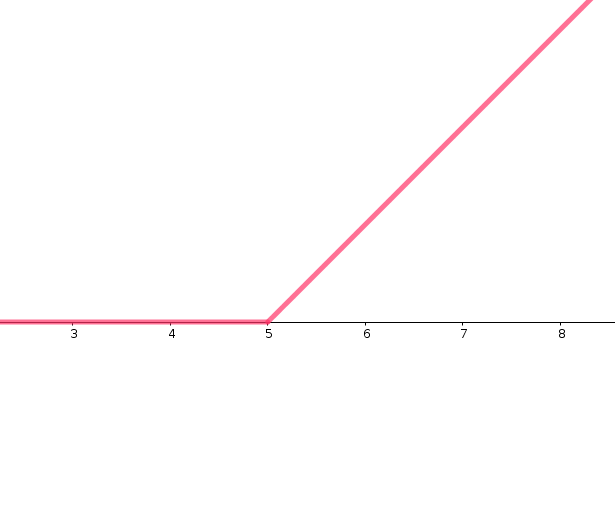
\includegraphics[width=6cm]{hinge} }}%
    \subfloat[$x\mapsto x\wedge 5$]{{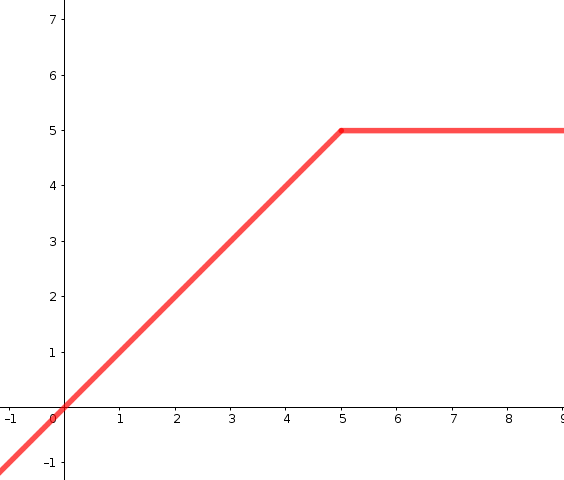
\includegraphics[width=6cm]{hingedeslocada} }}%
    \label{fig:example}%
\end{figure}

\end{proof}


\subsection{Sequências Previsíveis }


\begin{definition}[Sequência Previsível]\index{Sequência Previsível} Seja $(\F_n)$ uma filtração, dizemos que a sequência $(H_n)$ é previsível com relação à $(\F_n)$ se $H_n \in \F_{n-1}$. 
Além disso, vamos definir
$$(H,X)_n  =\sum^n_{m=1}H_m(X_m - X_{m-1}).  $$
\end{definition}

\begin{tcolorbox}[colback = yellow!60]
\begin{remark}
Note que podemos pensar em
$$ (H,X)_n = \sum^n_{m=1}H_m(X_m - X_{m-1})$$
como o ganho esperado na n-ésima rodada num jogo de aposta, sendo que temos uma estratégia $H_n$ para a rodada $n$ que depende apenas das rodadas anteriores. O que o teorema acima quer dizer, intuitivamente, é que num jogo desfavorável, independente da estratégia utilizada, o jogo sempre será desfavorável.
\end{remark}
\end{tcolorbox}

\begin{theorem}\label{teo- superm+previ+limit=HXsuper}
Seja $X_n$ um supermartingale, se $H_n\geq 0$ é previsível e cada $H_n$ é limitado, então $(H,X)_n$ é um supermartingale.
\end{theorem}
\begin{proof}
Basta notar que, como $H_n\geq 0,$
\begin{align*}
(H,X)_{n+1} & =\E\left(\sum_{m=1}^{n+1} H_m(X_m-X_{m-1})\left|\F_n\right. \right)\\
&=\left(\sum_{m=1}^{n} H_m(X_m-X_{m-1})\right) + \E(H_{n+1}(X_{n+1}-X_n)|\F_n)\\
& = (H,X)_n + \E(H_{n+1}X_{n+1}|\F_n) - \E(H_{n+1}X_n|\F_n)\\
& =(H,X)_n + H_{n+1}\E(X_{n+1}|\F_n) - H_{n+1}\E(X_n|\F_n)\\
& =(H,X)_n + H_{n+1}\E(X_{n+1}|\F_n) - H_{n+1}\E(X_n|\F_n)\\
&\leq (H,X)_n + H_{n+1}X_{n} - H_{n+1}X_n = 0. 
\end{align*}
E como $H$ é limitado, todos os passos anteriores fazem sentido.

\end{proof}

\begin{tcolorbox}[colback = yellow!60]
\begin{remark}
Note que \textbf{a mesma demonstração funciona para Martingales e submartingales}, sendo que no primeiro caso não precisamos que $H_n\geq 0$. Isso quer dizer que independentes da estratégia, um jogo neutro continua neutro e um jogo vantajoso continua vantajoso.
\end{remark}
\end{tcolorbox}

\subsection{Tempo de Parada}

\begin{definition}[Tempo de Parada]\label{def- tempo de parada} \index{Tempo de Parada}
Seja $\F_n$ a filtração natural dada a sequência $(X_n)$ de v.a.'s. Uma variável aleatório $N$ com valores em $\N\cup\{\infty\}$ é um tempo de parada se para todo $n<\infty$, temos que
$$\{N=n\}\in \F_n. $$
\end{definition}


\begin{remark}
Intuitivamente, se $N$ é uma v.a. que representa o momento em que um apostador deve parar de apostar, temos que $N\in \F_n$, já que essa decisão só depende do resultado da $n$-ésima rodada.
\end{remark}

\begin{lemma}
Seja $N$ um tempo de parada, então 
$$ H_n = 1_{n\leq N} $$
é previsível.
\end{lemma}
\begin{proof}
Note que 
$$\{N\leq n-1\} \in \F_{n-1}, $$
já que $N$ é tempo de parada. Como $\F_{n-1}$ é $\sigma$-álgebra, temos que 
$$\{N\geq n\} = \{N\leq n-1\}^c \in \F_{n-1}, $$
\end{proof}

\begin{theorem}\label{teo- super+stoptime=super} Se $X_n$ é um supermartingale e $N$ é um tempo de parada, então 
$$Y_n = X_{N\wedge n} $$
é um supermartingale . O mesmo vale para martingales e submartingales.
\end{theorem}


\begin{proof}
Basta usar o Teorema \ref{teo- superm+previ+limit=HXsuper} com $H_n = 1_{N\geq n},$ já que
$$(H,X)_n =  \sum^n_{m=1}1_{N\geq n}(X_m - X_{m-1}) = X_{N\wedge n} - X_0 $$
já que vamos apostar só enquanto $n\leq N$, isto é, ainda não for tempo de parada. É claro que sempre  $N\geq 0$.

Agora observe que $Y_n = X_0$ (sequência constante) é um supermartingale adaptado à $\F_n$ e que soma de supermartingales adaptados à $\F_n$ é supermartingale adaptado à $\F_n$, logo temos o resultado, já que
$$ X_{N\wedge n} = (H,X)_n + X_0. $$
\end{proof}
\begin{remark}
Isso quer dizer que em uma aposta não justa, mesmo impondo um tempo de parada, a aposta ainda é injusta. O mesmo vale para martingales.
\end{remark}






\subsection{Desigualdade dos Cruzamentos}



Sejam $a,b\in \R$ e  $(X_n)$ um submartingale tal que $a<b$. Defina $N_0=-1$
\begin{align*}
N_{2k-1} & = \inf\{m:\ m>N_{2k-2},\ X_m\leq a\},\\
N_{2k} & = \inf\{m:\ m>N_{2k-1},\ X_m\geq b\}
\end{align*}
Intuitivamente, podemos pensar em $(N_k)$ como
\begin{align*}
N_1 &= \textrm{Menor tempo em que o processo é menor que }a,\\
N_2 &= \textrm{Menor tempo em que o processo é maior que }b\\
& \textrm{(zeramos o relógio)}\\
N_3 &= \textrm{Menor tempo em que o processo é menor que }a,\\
N_4 &= \textrm{Menor tempo em que o processo é maior que }b\\
& \textrm{(zeramos o relógio)}\\
N_5 &= \textrm{Menor tempo em que o processo é menor que }a,\\
N_6 &= \textrm{Menor tempo em que o processo é maior que }b\\
&\vdots
\end{align*}
Ou seja, cada par $N_{2k-1}, N_{2k}$ define um cruzamento completo do intervalo $(a,b)$.
Abaixo exibimos uma ilustração.


\begin{figure}[h]
\centering % para centralizarmos a figura
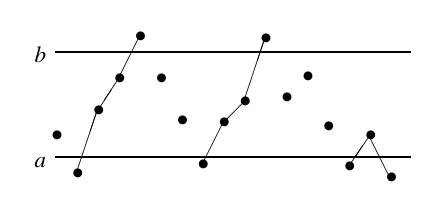
\includegraphics[width=10cm]{upcrossing} % leia abaixo
\caption{Retirado de \cite{durrett}. }
\end{figure}
 

\begin{lemma}
$N_k,\ k= 1,2,\dots$ como acima são tempos de parada.
\end{lemma}
\begin{proof}
Intuitivamente é claro, já que $\{N_j=k\}$ só depende do valor de $(X_n)$ no tempo $k.$
Para uma prova formal, observe que
\begin{align*}
\{ N_1 =k_1 \} &= \{ X_1> a, X_2> a,\dots, X_{k_1}\leq a  \}\in \F_{k_1}\\
\{ N_2 =k_2 \} &= \bigcup_{k_1<k_2} (\{N_1=k_1\}\cap \{X_{k_1+1}<b,\dots,X_{k_2}\geq b\} )\in \F_{k_2}.\\
\{ N_3 =k_3 \} &= \bigcup_{k_1<k_2<k_3} (\{N_1=k_1\}\cap\{N_2 = k_2\}\cap \{X_{k_2+1}>a,\dots,X_{k_3}\leq a\} )\in \F_{k_1}.
\end{align*}
E é fácil generalizar esse argumento indutivamente.
\end{proof}





\begin{lemma}\label{lema-H-estrategia cruzamento}
Defina
$$H_m = \begin{cases}
1,\   & \textrm{se } N_{2k-1}<m\leq N_{2k},\  \textrm{para algum }k,\\
0,&\ \textrm{caso contrário }.
\end{cases} $$
Então $(H_n)$ é uma sequência previsível.
\end{lemma}
\begin{proof}
Note que
\begin{align*}
\{N_{2k-1}<m\leq N_{2k}\} &= \{N_{2k-1}<m\}\cap \{m\leq N_{2k}\}\\
& = \{N_{2k-1}\leq m-1\}\cap \{ N_{2k} > m-1 \}^c.
\end{align*}
\end{proof}


\begin{remark}
Note que $(H_n)$ é a estratégia que só aposta  caso estejamos num tempo intermediário entre cruzamentos do intervalo $(a,b)$. Isso faz muito sentido pensando num mercado de ações, por exemplo.
\end{remark}

\begin{figure}[H]
\centering % para centralizarmos a figura
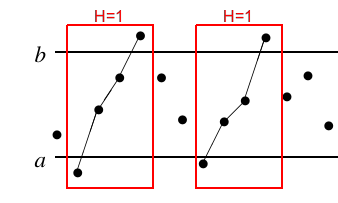
\includegraphics[width=10cm]{upcrossingHn} % leia abaixo
\caption{Fora dos retângulos vermelhos, $H=0$.}
\end{figure}
 




\begin{theorem}[Desigualdade dos Cruzamentos - \cite{durrett}]\label{teo-desicruzamentos}\index{Teorema! Desigualdade dos Cruzamentos}
\index{Desigualdade! dos Cruzamentos}
\index{Teorema! Desigualdade dos Cruzamentos}

Seja $(X_n)$ um \textbf{submartingale} e $a<b$. Então
\begin{align*}
(b-a)\E U_n &\leq  \E(a+(X_n-a)^+) - \E(a+(X_0-a)^+)\\
&=\E(X_n-a)^+ - \E(X_0-a)^+,
\end{align*}
onde 
$$U_n = \sup\{k:\ N_{2k}\leq n\}, $$
isto é, $U_n$ conta a quantidade de cruzamentos do intervalo $(a,b)$ até o tempo $n$.
\end{theorem}


\begin{proof}
Seja 
$$ Y_n = a + (X_n-a)^+,$$
isto é, 
$$\begin{cases}
Y_n &= a \text{ se } X_n\leq a\\
Y_n &= X_n\text{ se }X_n\geq a.
\end{cases} $$


Como $(X_n)$ é submartingale, já vimos que $(X_n-a)^+$ é um submartingale. E como o processo constante $(a)$ é um martingale, temos que \textbf{$Y_n$ é um submartingale}.
Considere $K = 1-H$, isto é, a estratégia complementar de $H$ (aposta quando $H$ não aposta), onde $H$ é como no Lema \ref{lema-H-estrategia cruzamento}. É fácil ver que
$$Y_n-Y_0 = (H,Y)_n + (K,Y)_n. $$ 
Como $(Y_n)$ define um jogo favorável, sabemos que $(H,Y)_n$ e $(K,Y)_n$ são estratégias favoráveis, já que $H,K\geq 0$ e ambos são limitados. Temos então que
$Y_n - Y_0 $ é um submartingale.

Agora note que
$$U_n (b-a) \leq  (H,Y)_n $$
já que cada cruzamento contribui com pelo menos $(b-a)$. E mais, se $n$ é impar, ou seja, não terminamos um ciclo de aposta, então a contribuição desse último ciclo é não negativa, pois $Y_n\geq a$ e $H$ só aposta se estivermos com ganho $\geq 0$.
Além disso, como $(K,Y)_n$ é submartingale,
$$\E((K,Y)_n)\geq \E((K,Y)_0) \geq 0 . $$

Por fim, juntando todos esses fatos,
\begin{align*}
(b-a)\E(U_n) & \leq \E((H,Y)_n) + 0\\
& \leq \E((H,Y)_n) + \E((K,Y)_n)\\
& = \E((H,Y)_n + (K,Y)_n)\\
& = \E(Y_n - Y_0).
\end{align*}
\end{proof}



\subsection{Convergência de Martingales}


\begin{theorem}[Teorema da Convergência de Martingales-\cite{durrett}]\label{teo-conv-martings} \index{Teorema! Convergência de Martingales}
 Seja $(X_n)$ um \textbf{submartingale} com 
$$ \sup \E X_n^+ <\infty. $$
Então, 
$$X_n \rarrowlimn X,\ q.t.p. $$
para uma v.a. $X$ com $\E|X|<\infty.$
\end{theorem}
\begin{proof}
Primeiramente, fixe $a<b$ e note que $(U_n)$ é uma sequência monótona e positiva. Logo, pelo teorema da convergência monótona
$$\E(U) = \lim_n\E(U_n), $$
onde $U = \lim_n U_n,$ é a v.a. que conta todos os cruzamentos da sequência $(X_n).$
$$\E(U) = \lim_n\E U_n \leq\lim_n \dfrac{\E(X_n-a)^+}{b-a}\leq \lim_n\dfrac{\E X_n^+ + |a|}{b-a}\leq \dfrac{\sup_n \E X_n^+ + |a|}{b-a}<\infty.$$
Portanto, temos que $U<\infty$ q.t.p.

Agora, supondo que $a,b\in \mathbb{Q}$, observe que
$$A_{a,b}= \{ \limsup X_n \geq b>a\geq \liminf X_n \}$$
tem medida nula, pois se não, haveria um conjunto de medida positiva com infinitos cruzamentos do intervalo $(a,b)$, contrariando o fato de que $U<\infty.$

É claro que, então 
$$A = \bigcup_{a,b\in \mathbb{Q},a<b} A_{a,b} $$
tem medida nula. Em particular
$$\{\limsup X_n > \liminf X_n \} =\{\limsup X_n = \liminf X_n\}^c $$
tem medida nula, isto é, $(X_n)$ converge para uma v.a. $X$ q.t.p.

Como
\begin{align*}
 |X_n| &= X_n^+ + X_n^-\\
 X_n   &= X_n^+ - X_n^-, 
\end{align*}
temos que
$$|X_n| = 2X_n^+ - X_n. $$
Como $(X_n)$ é submartingale, temos que
$$-\E(X_n) \leq -\E(X_0),$$
e portanto, utilizando o lema de Fatou,
\begin{align*}
\E(|X|) &\leq \liminf\E(|X_n|)\\
& \leq \liminf 2\E(X_n^+) - \E(X_0)\\
& \leq \limsup 2\E(X_n^+) - \E(X_0)<\infty,
\end{align*}
provando então que $\E|X|<\infty.$
\end{proof}



\begin{theorem}
Seja $(X_n)$ um supermartingale com $X_n\geq 0$, então 
$$X_n \rarrowlimn X,\ q.t.p.$$
e $\E X\leq \E X_0.$
\end{theorem}

\begin{proof}
Temos que $(-X_n)$ é um submartingale, com $-X_n\leq 0$ e portanto $(-X_n)^+ = 0.$ Pelo teorema \ref{teo-conv-martings}, temos que $X_n \rarrowlimn X$ q.t.p. para uma v.a. $X$ com $\E |X|<\infty.$

Como $(X_n)$ é um supermartingale, temos que
$$\E(X_n)\leq \E(X_0) $$
e o resultado segue pelo lema de Fatou.
\end{proof}




\begin{tcolorbox}
\begin{example}[O teorema anterior \textbf{NÃO} garante convergência $L^1$]
Considere o caso de um passeio aleatório simétrico $(S_n)$ com $S_0 = 1$. Defina 
$$N= \inf\{n: S_n = 0 \}, $$
e  também,
$$X_n = S_{N\wedge n}. $$
Como vimos no teorema \ref{teo- super+stoptime=super}, $X_n$ é um  Martingale. Além disso, $X_n$ é não negativo devido ao fato de que $S_0=1$ e a a condição do tempo de parada.

Portanto, pelo teorema anterior,  $X_n \rarrowlimn X,\ q.t.p.$.
Note que $X=0,$ q.t.p., pois caso contrário, se $X=k>0$, teríamos que para $n$ grande
$$X_n = k>0\ \textrm{e}\ X_n = k\pm 1. $$

Resumindo, temos que $X_n \rarrowlimn 0,$ q.t.p., porém $\E(X_n) = \E(X_0)=1$, e então não podemos ter convergência em $L^1.$
\end{example}
\end{tcolorbox}




\begin{example}
Considere $S_n$ um random walk simples e tome $a\leq 0$ qualquer. Considere também o tempo de parada 
$$N = \inf\{k: S_k = a\}.$$
Então, já vimos que o processo $(Y_n) = (S_{n\wedge N})$ é um martingale.
É claro que 
$$Y_n-a \geq 0$$
e portanto, pelo corolário anterior, temos que 
$$Y_n \rarrowlimn Y,\ \textrm{q.t.p.} $$
com $Y$ v.a. finita q.t.p. já que $\E|Y|<\infty$.
Em particular,
$$|Y_{n+1}-Y_n| \rarrowlimn 0 $$ 
mas como os valores de $(Y_n)$ são discretos, isso significa que para $n$ suficientemente grande $Y_{n+1}=Y_n$ o que se pode acontecer se $N<\infty$ q.t.p.. 
\end{example}
















\newpage
\section{Convergência de Martingales: Rota Alternativa}

Abaixo exibimos uma formulação alternativa para a desigualdade dos cruzamentos e para o teorema de convergência. A principal diferença é que vamos pedir que $\sup \E |X_n|<\infty$ ao contrário da versão anterior em que pedimos $\sup \E (X_n)^+<\infty$

\begin{theorem}[Desigualdade dos Cruzamentos - \cite{williams-martingales}]\label{teo-desicruzamentos-will}\index{Teorema! Desigualdade dos Cruzamentos}
\index{Desigualdade! dos Cruzamentos}
\index{Teorema! Desigualdade dos Cruzamentos}

Seja $(X_n)$ um \textbf{supermartingale} e $a<b$. Então
\begin{align*}
(b-a)\E U_n &\leq \E(X_n-a)^-
\end{align*}
onde 
$$U_n = \sup\{k:\ N_{2k}\leq n\}, $$
isto é, $U_n$ conta a quantidade de cruzamentos no intervalo $[a,b]$ até o tempo $n$.
\end{theorem}
\begin{proof}
Considere  $H$ como no Lema \ref{lema-H-estrategia cruzamento}. Note que
$$(H,X)_n \geq (b-a)U_n - (X_n-a)^-, $$
já que o  lucro total ($(H,X)_n)$) é pelo menos $(b-a)$ vezes a quantidade de cruzamentos $U_n$, porém precisamos descontar um possível prejuízo da rodada $n$ já que esta possivelmente foi interrompida antes de haver um cruzamento. 

Como $(X_n)$ é supermartingale, temos que $(H,X)_n$ é supermartingale, logo 
$$\E(H,X)_n \leq \E(H,X)_0 :=0 $$
e portanto
$$(b-a)\E(U_n) \leq \E(X_n-a)^-. $$
\end{proof}

\begin{theorem}[Teorema da Convergência de Martingales-\cite{williams-martingales}]\label{teo-conv-martings-will} \index{Teorema! Convergência de Martingales}
 Seja $(X_n)$ um \textbf{supermartingale} com 
$$ \sup \E |X_n| <\infty. $$
Então, 
$$X_n \rarrowlimn X,\ q.t.p. $$
para uma v.a. $X$ com $\E|X|<\infty.$
\end{theorem}
\begin{proof}

Primeiramente, fixe $a<b$ e note que $(U_n)$ é uma sequência monótona e positiva. Logo, pelo teorema da convergência monótona
$$\E(U) = \lim_n\E(U_n), $$
onde $U = \lim_n U_n,$ é a v.a. que conta todos os cruzamentos da sequência $(X_n).$
$$\E(U) = \lim_n\E U_n \leq\lim_n \dfrac{\E(X_n-a)^-}{b-a}\leq  \dfrac{\sup_n \E |X_n| + |a|}{b-a}<\infty.$$
Portanto, temos que $U<\infty$ q.t.p.

Agora, supondo que $a,b\in \mathbb{Q}$, observe que
$$A_{a,b}= \{ \limsup X_n \geq b>a\geq \liminf X_n \}$$
tem medida nula, pois se não, haveria um conjunto de medida positiva com infinitos cruzamentos do intervalo $(a,b)$, contrariando o fato de que $U<\infty.$

É claro que, então 
$$A = \bigcup_{a,b\in \mathbb{Q},a<b} A_{a,b} $$
tem medida nula. Em particular
$$\{\limsup X_n > \liminf X_n \} =\{\limsup X_n = \liminf X_n\}^c $$
tem medida nula, isto é, $(X_n)$ converge para uma v.a. $X$ q.t.p.

Para finalizar, pelo lema de Fatou,
\begin{align*}
\E(|X|) &\leq \liminf\E(|X_n|)<\infty,
\end{align*}
provando então que $\E|X|<\infty.$
\end{proof}




\begin{tcolorbox}[colback = yellow!60]
Note que no teorema de convergência \ref{teo-conv-martings} pedimos que $(X_n)_n$ seja um submartingale, porém em \ref{teo-conv-martings-will} pedimos que $(X)n)_n$ seja um supermartingale. É claro que tomando $(Y_n)_n = (-X_n)_n$ conseguimos mostrar que tanto faz usarmos submartingales ou supermartingales.

O único motivo para essas hipóteses serem diferentes é que utilizamos fortemente a desigualdade dos cruzamentos e a estratégia de prova das duas versões é levemente diferente, já que no primeiro caso conseguimos um resultado mais geral.
\end{tcolorbox}





\subsection{Decomposição de Doob}

\begin{tcolorbox}
\begin{theorem}[Decomposição de Doob]\index{Teorema! Decomposição de Doob}\index{Doob! Decomposição } \label{teo-decomp-Doob} Seja $(X_n)$ um processo adaptado à $(\F_n)$ com $(X_n) \subset L^1$. Então $(X_n)$ pode ser escrito unicamente como
$$X_n =X_0 +  M_n + H_n, $$
onde $M_n$ é um Martingale nulo em $n=0$, $H_n$ é uma sequência previsível nula em $n=0$. Além disso, $(X_n)$ é um submartingale se, e só se, $H_n$ é crescente.
\end{theorem}
\end{tcolorbox}

\begin{proof}
Se a decomposição existir, então
$$\E(X_n|\F_{n-1}) = X_0+ \E(M_n|\F_{n-1}) + \E(H_n|\F_{n-1}) =X_0+  M_{n-1} + H_n. $$
Como 
$$ M_{n-1} = X_{n-1} - H_{n-1}-X_0, $$
temos que
$$\E(X_n|\F_{n-1}) = X_{n-1} - H_{n-1} + H_n .$$
Ou seja, temos duas relações:
\begin{enumerate}
\item $H_n - H_{n-1} = \E(X_n|\F_{n-1}) -X_{n-1}$,
\item $M_n= X_n - H_n.$ 
\end{enumerate}
Definindo então $H_0=M_0 = 0$, o item 1 nos dá uma receita para construir $H_n$ unicamente, a menos de versões equivalentes da mesma v.a.. Note que como
$$H_n = \E(X_n|\F_{n-1}) - X_{n-1 } + H_{n-1}, $$
indutivamente, conseguimos mostrar que $H_n\in \F_{n-1}$.
Além disso, pelo item 1, é fácil ver  que $(H_n)$ é crescente se, e só se, $(X_n)$ é submartingale.

Uma vez construído a sequência previsível $(H_n)$, conseguimos construir $M_n$ unicamente pelo item 2. 

Note que $M_n$ é um Martingale,  já que
\begin{align*}
\E(M_n|F_{n-1}) &=  \E(X_n|F_{n-1})-\E(H_n|F_{n-1})\\
& =  \E(X_n|F_{n-1}) - H_n\\
& \underset{\textrm{Item 1.}}{=} X_{n-1}-H_{n-1} \\
& \underset{\textrm{Item 2.}}{=} M_{n-1}. 
\end{align*}

\end{proof}



\newpage
\section{Desigualdade de Doob e Convergência $L^p$}



\begin{theorem}
Se $(X_n)$ é um submartingale e $N$ é um tempo de parada limitado por $k$, então
$$\E X_0 \leq \E X_N \leq E X_k $$
\end{theorem}
\begin{remark}
Intuitivamente, é claro que  esse resultado deve ser verdadeiro.
\end{remark}


\begin{proof}
 Já vimos que $(X_{N\wedge n})$ também é um submartingale, logo 
 $$\E X_0 = \E X_{N\wedge 0} \leq \E X_{N\wedge k} = \E X_N,  $$
 provando a primeira desigualdade. 
 
Agora considere a sequência previsível e limitada $H_n = 1_{N\leq n-1}$, isto é, apostamos só quando $n>N$. Temos então que 
$$(H,X)_n = X_{n}- X_{N\wedge n} $$
 é um submartingale e portanto
 $$ = \E(X_k) - \E(X_N) =  \E(X,H)_k\geq |E(X,H)_0 = 0$$
\end{proof}






\begin{theorem}[Desigualdade de Doob] \label{teodesigdoob} \index{Teorema! Desigualdade de Doob} \index{Desigualdade! Doob} \index{Doob! Desigualdade}
Sejam $(X_n)$ um submartingale, $\lambda>0$ e
$$X_n'  = \max_{0\leq m\leq n}X_n^+.$$
Então
$$\pr (X_n'\geq \lambda)\leq \dfrac{\E (X_n 1_{X_n'\geq \lambda}) }{\lambda}\leq \E X_n^+. $$
\end{theorem}
\begin{proof}
Defina o tempo de parada
$$N = \inf\{m: X_m \geq \lambda \textrm{ ou } m=n \}, $$
isto é, $N$ marca o menor tempo em que o processo fica maior que $\lambda$ até o processo acabar no tempo $n$. Como $N$ é limitado por $n$, temos pelo teorema anterior que
$$\E(X_N) \leq \E(X_n). $$ 
Note que  no evento $\{X_n'\geq \lambda\}$ temos que $X_N\geq \lambda $ e então
$$\lambda \pr({X_n'\geq \lambda}) \leq \E(X_N 1_{X_n'\geq \lambda} ). $$
Além disso, temos que
\begin{align*}
\E(X_N) &= \E(X_N 1_{X_n'\geq \lambda}) + \E(X_N 1_{X_n'< \lambda})\\
& = \E(X_N 1_{X_n'\geq \lambda}) +\E(X_n 1_{X_n'< \lambda})\\
& = \E(X_N 1_{X_n'\geq \lambda}) + \E (X_n) - \E(X_n 1_{X_n'\geq \lambda})
\end{align*}
e portanto, como $\E(X_N)\leq \E(X_n)$
$$\E(X_N 1_{X_n'\geq \lambda})  \leq \E(X_n 1_{X_n'\geq \lambda}).  $$

Com isso temos que

$$\lambda \pr({X_n'\geq \lambda}) \leq \E(X_n  1_{X_n'\geq \lambda} ). $$

E a segunda desigualdade do enunciado é trivial.
\end{proof}






\begin{tcolorbox}

\begin{example}[Desigualdade Maximal de Kolmogorov]\label{teo-desi-maxikolm-martin}\index{Desigualdade! Maximal de Kolmogorov}\index{Kolmogorov! Desigualdade Maximal}\index{Teorema! Desigualdade Maximal de Kolmogorov} Vamos apresentar uma prova alternativa para a Desigualdade Maximal de Kolmogorov \ref{teo-desiMaxKolmo}.
\bigskip

Considere então $(X_n)$ v.a.'s independentes com média 0. Sabemos que $(S_n)$ é um martingale, e portanto $(S_n^2)$ é um submartingale já que $x\mapsto x^2$ é convexa.

Temos então pelo teorema anterior que, tomando $\lambda= x^2$
$$\pr\left(\max_{0\leq m\leq n} |S_m|\geq x \right) \leq \dfrac{\Var(S_n)}{x^2}. $$
\end{example}

\end{tcolorbox}









\newpage
\section{Exercícios Resolvidos}
\begin{xca}[\cite{durrett}] Prove a Desigualdade de Chebyshev no caso condicional, isto é,
$$\pr(|X|>a|\mathcal{F})\leq \dfrac{\E(X^2|\mathcal{F})}{a^2},\ a>0. $$
\end{xca}

\begin{proof}
Basta notar que
$$a 1_{|X|> a}\leq |X|. $$
\end{proof}

\begin{xca}[\cite{durrett}]
Sejam $X,Y$ v.a.'s  com $\E(Y|\mathcal{G}) = X$ e $\E Y^2 = \E X^2$. Mostre que $X=Y$ q.t.p..
\end{xca}
\begin{proof}
Como $\E(Y|\mathcal{G}))=X$ é claro que $X\in \mathcal{G}$. Então
$$\E(X^2) = \E(X\E(Y|\mathcal{G})) = \E(\E(XY|\mathcal{G})) = \E(XY).$$
Mas então
\begin{align*}
\E((X-Y)^2) & = \E(X^2 -2XY + Y^2) = 0.
\end{align*}
\end{proof}





\newpage
\chapter{Probabilidade em Espaços Métricos e Movimento Browniano}


\section{Convergência}

\begin{tcolorbox}

\begin{definition}[Convergência Fraca] Seja $(\Omega,\mathcal{B})$ um espaço de probabilidade onde $\Omega$ é um espaço métrico com distância $d$ e $\mathcal{B}$ é a $\sigma$-álgebra de Borel gerada por $d.$ Dado uma sequência de probabilidades $\mu_n$ em $(\Omega,\mathcal{B})$, dizemos que $\mu_n$ converge fracamente para $\mu$ se 
$$\int f(x)d\mu_n(x) \rightarrow \int f(x)d\mu(x), $$
para toda função $f$ contínua e limitada. Simbolizamos essa convergência como 
$\mu_n \Rightarrow \mu. $

Da mesma Forma, se $(X_n)$ é uma sequência de v.a.'s, dizemos que $X_n$ converge fracamente para $X$ (ou que converge em lei) se
$$\E f(X_n)\rightarrow \E f(X), $$
para toda função $f$ contínua e limitada. Simbolizamos essa convergência como 
$X_n \Rightarrow X. $
\end{definition}

\end{tcolorbox}












\newpage
\section{Exercícios Resolvidos}











\part{Apêndice}

\appendix
\chapter{}

\section{Fórmula de Stirling}\label{sec-stirling} \index{Stirling, Fórmula de}
\begin{tcolorbox}[colback = white]
As Principais referências usadas foram:
\begin{enumerate}
\item \cite{taomatrix}
\item \cite{spencer-asymtopia}
\item \cite{keith-stirling}
\end{enumerate}
\end{tcolorbox}

\begin{tcolorbox}[colback = yellow!60]

O nosso objetivo é mostrar a seguinte identidade assintótica:
\begin{equation}
n!\sim \sqrt{2\pi n}\left( \dfrac{n}{e}\right)^n.
\end{equation}\label{stirling-formula}

\end{tcolorbox}

\begin{lemma}
Temos que
$$n! = \int_0^{+\infty} t^n e^{-t}dt . $$
\end{lemma}

\begin{proof}
Integrando por partes uma vez, temos que
$$\int_0^{+\infty} t^n e^{-t}dt = \left( e^{-t}t^n\right)\Big|^{\infty}_0 +n\int_0^{+\infty} t^{n-1} e^{-t}dt.$$
Então o resultado sai por indução.
\end{proof}

\begin{lemma}
A função $$f(t) = t^ne^{-t}$$
atinge máximo em $t=n$.
\end{lemma}

Abaixo, exibimos o gráfico da função $$ f(t) = t^ne^{-t},$$
para diversos valores de $n.$ Note que todos os gráficos, possuem o mesmo aspecto de sino quando observados em torno do máximo de $f(t)$. 

\begin{figure}[h]
\centering
    \subfloat[Para $n=5$]{{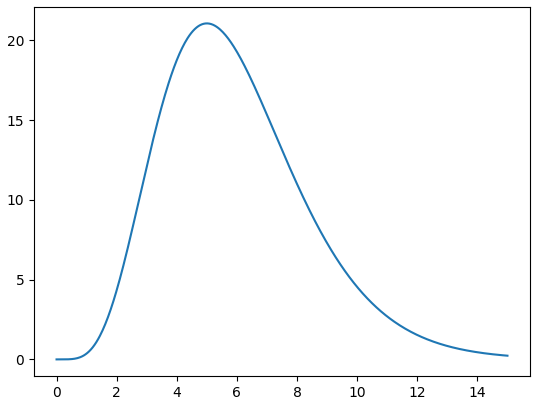
\includegraphics[width=6.5cm]{bellshapedn5} }}%
    \subfloat[Para $n=50$]{{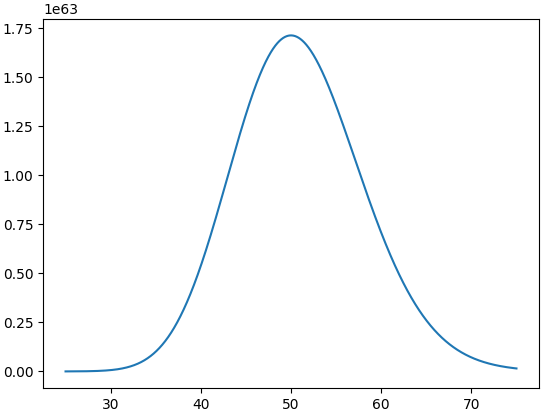
\includegraphics[width=6.5cm]{bellshapedn50} }}%
    
    \subfloat[Para $n=100$]{{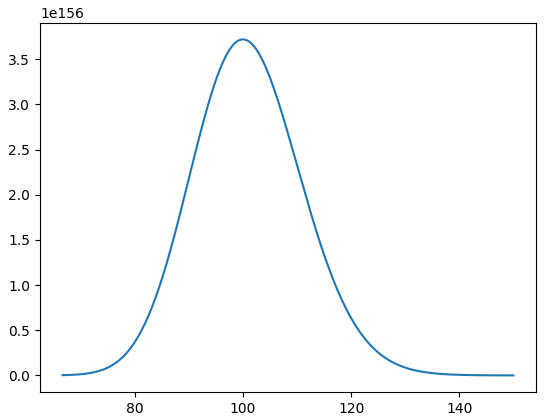
\includegraphics[width=7cm]{bellshapedn100} }}%
    \caption{Gráfico de $f(t)= t^ne^{-t}.$}%
    \label{fig:example}%
\end{figure}

Façamos então uma mudança de coordenadas que leve em consideração esse fato, isto é, vamos, vamos integrar com respeito á $t = s+n$:

\begin{align*}
n! &= \int_0^{+\infty} t^n e^{-t}dt \\
 &=\int_{-n}^{+\infty} (s+n)^n e^{-(s+n)}ds \\
 &=\left(\dfrac{n}{e}\right)^n\int_{-n}^{+\infty} \left(1+\dfrac{s}{n}\right)^n e^{-s}ds\\
 &=\left(\dfrac{n}{e}\right)^n\int_{-n}^{+\infty}  \exp\left(-s+n\ln\left(1+\dfrac{s}{n}\right)\right) ds 
\end{align*}
\begin{tcolorbox}[colback = yellow!60] \textbf{Intuição: }
Como para $|s|<n,$
$$n\ln\left(\dfrac{s}{n}+1\right) = s -\dfrac{s^2}{2n}+\dots, $$
fazendo  a mudança de coordenadas $s = t\sqrt{n}$:
\begin{align*}
n! &=  \left(\dfrac{n}{e}\right)^n\int_{-n}^{+\infty}  \exp\left(-s+n\ln\left(1+\dfrac{s}{n}\right)\right) ds \\
&\approx\left(\dfrac{n}{e}\right)^n\int_{-n}^{+\infty}  \exp\left(-\dfrac{s^2}{2n}\right) ds.\\
& = \left(\dfrac{n}{e}\right)^n \sqrt{n}\int_{-\sqrt{n}}^{+\infty}  \exp\left(-\dfrac{t^2}{2}\right) dt.\\
& \sim \sqrt{2\pi n} \left(\dfrac{n}{e}\right)^n .
\end{align*}
\end{tcolorbox}
Para formalizar a intuição acima, considere a mudança de variáveis $s=t\sqrt{n}$. Então
\begin{align*}
n! &=\left(\dfrac{n}{e}\right)^n\sqrt{n}\int_{-\sqrt{n}}^{+\infty}  \exp\left(-t\sqrt{n}+n\ln\left(1+\dfrac{t}{\sqrt{n}}\right)\right) dt .
\end{align*}
\begin{lemma}
 Temos que
$$\exp\left(-t\sqrt{n}+n\ln\left(1+\dfrac{t}{\sqrt{n}}\right)\right) \rarrowlimn e^{-t^2/2}. $$
\end{lemma}
\begin{proof}
Como $t$ é fixo, basta estudarmos o que acontece quando $n$ é bem maior que $t$. Suponha então que $n>t^2$, isto é, $|t/\sqrt{n}|<1$.

Então,
\begin{align*}
n\ln\left(\dfrac{t}{\sqrt{n}}+1\right) - \sqrt{n}t &= n\left(-\dfrac{t^2}{2n}+O((t/\sqrt{n})^3)\right)\\
&=-\dfrac{t^2}{2}+O(t^3/\sqrt{n})\rarrowlimn -t^2/2.
\end{align*}
\end{proof}
Defina,
$$f_n(t) := 1_{[-\sqrt{n}, +\infty )}\exp\left(-t\sqrt{n}+n\ln\left(1+\dfrac{t}{\sqrt{n}}\right)\right). $$
Então só o que nos falta mostrar é que
$$\lim_n \int f_n(t)dt = \int \lim_n f_n(t)dt = \int e^{-t^2/2}dt. $$


\begin{lemma} 
Existe uma função mensurável  $g$ com módulo integrável, tal que $|f_n|< g$. Portanto, pelo teorema da convergência dominada,
$$ \int_{-\sqrt{n}}^{+\infty}  \exp\left(-t\sqrt{n}+n\ln\left(1+\dfrac{t}{\sqrt{n}}\right)\right) dt \rarrowlimn \int e^{-t^2/2}dt  = \sqrt{2\pi}.$$
\end{lemma}

\begin{proof} Já vimos que 
$$\log f_n(t) = -t^2/2 + O(t^3/\sqrt{n}), $$
note que se $t<0$, intuitivamente
$$\log f_n(t) = -t^2/2 + O(t^3/\sqrt{n})< -t^2/2, $$
já que $O(t^3/\sqrt{n})<0$.

Se $t>0$, intuitivamente, temos que 
$$-\dfrac{t^2}{2} + \dfrac{t^3}{\sqrt{1}} > \dfrac{t^2}{2} +  \dfrac{t^3}{\sqrt{2}} > \dots > \dfrac{t^2}{2} +  \dfrac{t^3}{\sqrt{n}} > \dots , $$
isto é, $f_n\leq f_1=(1+t)e^{-t}.$

Defina $g$ como
$$g(t) = 
     \begin{cases}
       e^{-t^2/2} &\text{se } -\sqrt{n}\leq  t<0,\\
      (1+t)e^{-t} &\text{se } t\geq 0.
     \end{cases}. $$

De fato, não é difícil mostrar que $|f_n|\leq g$ e que $g$ é integrável  ( usar técnicas simples de cálculo), portanto, pelo teorema da convergência dominada, como $f_n \rarrowlimn e^{-t^2/2},$ temos o resultado.
\end{proof}






\newpage
\section{Expansão de Padé}\index{Expansão de Padé}

\begin{tcolorbox}[colback = white]
As principais referências usadas foram: 
\begin{enumerate}
\item \cite{MathewsNumericalMethodsMatlab}.
\item \cite{geogebra}.
\end{enumerate}
\end{tcolorbox}

Quando provamos a desigualdade de Bernstein, utilizamos o seguinte fato:
$$(1+x)\log(1+x)-x \geq \dfrac{x^2}{2(1+x/3)}, $$
provar que essa desigualdade vale é um exercício normal de cálculo, a questão fundamental é: como alguém pode deduzir tal desigualdade?

Note que, assim como numa expansão de Taylor, estamos aproximando 
$$f(x)=(1+x)\log(1+x)-x$$ por funções mais simples, isto é, quocientes de polinômios.

Em geral, suponha que
$$f(x) = \sum_{i=0}^\infty a_ix^i ,$$
e que queremos escrever \footnote{ou mais informalmente
$f(x)\approx \dfrac{p(x)}{q(x)}. $}
$$f(x)q(x) = p(x) + z(x) , $$
onde $p(x)$ é um polinômio de grau $n$, $q(x)$ é um polinômio de grau $m$ e as derivadas de $f$ e  $r(x):=p(x)/q(x)$ coincidam em $0$ até o grau $n+m$.

Note que, pela condição das derivadas coincidirem em $0$ até  $n+m$, é fácil ver que $z(x)$ tem que ser da forma:
$$z(x) = \sum_{i=n+m+1}^\infty z_ix^i. $$
Além disso, como estamos expandindo $f$ em torno do $0$, queremos que o $q(0)\neq 0$, logo, podemos supor que $q_0=1$. Portanto: 
$$\left(\sum_{i=0}^\infty a_ix^i \right)\left(1+\sum_{i=1}^m q_ix^i\right) -\sum_{i=0}^n p_ix^i =  \sum_{i=n+m+1}^\infty z_ix^i.$$ 
Dessa forma, conseguimos um sistema linear de $n+m+1$ incógnitas que podemos resolver para encontrarmos os coeficientes $q_i,p_i$. Abaixo, exibimos as 4 primeiras equações lineares, que vamos chamar de \emph{equações de Padé}:
\begin{align*}\label{pade}
a_0-p_0&=0\\
q_1a_0+a_1-p_1&=0\\
q_2a_0+q_1a_1+a_2-p_2 &= 0\\
q_3a_0+q_2a_1+q_1a_2+a_3-p_3&=0.
\end{align*}

Com as quatro equações acima, já somos capazes de aproximar $f(x)$ por  funções da forma $p(x)/q(x)$ com $p$ de grau $2$ e $q$ de grau $1$. Por exemplo, considere novamente
$$ f(x)=(1+x)\log(1+x)-x,$$
é fácil\footnote{Wolfram =)} ver que
$$f(x) = 0 + 0x + x^2/2 - x^3/6 + \cdots, $$
e então, substituindo os coeficientes $a_i$ de $f$ nas equações de Padé, temos que
 \begin{align*}
0-p_0&=0 \longrightarrow p_0 = 0\\
0q_1+0-p_1&=0 \longrightarrow p_1 = 0\\
0q_2+0q_1+1/2-p_2 &= 0\longrightarrow p_2 = 1/2\\
0q_3+0q_2+q_1/2-1/6-0&=0\longrightarrow q_1 = 1/3,
\end{align*}
e podemos concluir que
$$f(x) \approx \dfrac{x^2/2}{1+x/3}, $$
que nos leva exatamente à desigualdade que precisamos, como ilustrado abaixo \footnote{Imagens geradas no Geogebra \cite{geogebra}.} 
\begin{figure}[h]
\centering % para centralizarmos a figura
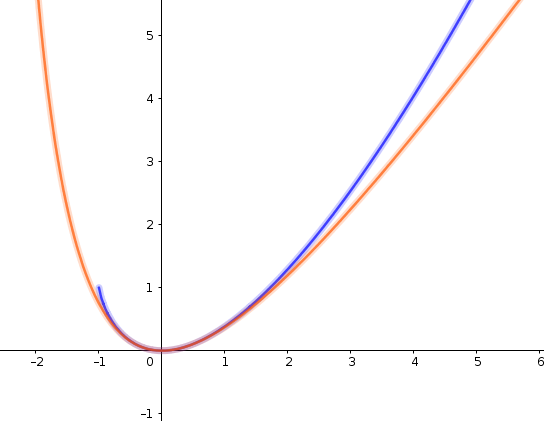
\includegraphics[width=8cm]{1xl1x-x} % leia abaixo
\caption{Em azul temos $(1+x)\log(1+x)-x$ e em vermelho $\dfrac{x^2/2}{1+x/3}$.}
\end{figure}
 



Façamos mais um exemplo, dessa vez para 
$$g(x) = 1+x - \sqrt{1+2x} = 0 + 0x + x^2/2 - x^3/2 + \cdots,$$ e então resolvendo as equações de Padé, temos que
$$g(x)\approx \dfrac{x^2/2}{1+x}, $$
e é possível mostrar que podemos trocar $\approx$ por $\geq$. 

\begin{figure}[h]
\centering % para centralizarmos a figura
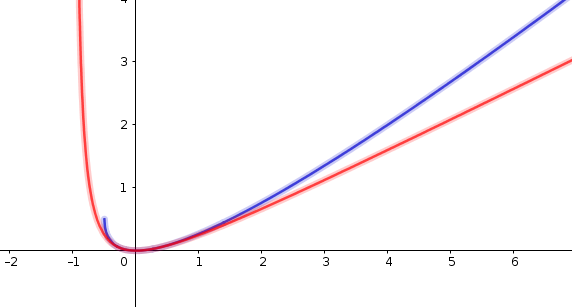
\includegraphics[width=10cm]{1xsqrt} % leia abaixo
\caption{Em azul temos $1+x - \sqrt{1+2x}$ e em vermelho $ \dfrac{x^2/2}{1+x}$. }
\end{figure}
 





Para finalizar, já sabemos que
$$\dfrac{x}{x+1}\leq \log(1+x),\ \ \ \ x>-1, $$
mas então, para $x\in(0,1)$, temos que
$$ -\log(1-x)-x \leq \dfrac{x}{-x+1}-x = \dfrac{x^2}{1-x}.$$
Utilizando a aproximação de Padé, conseguimos encontrar um bound com uma constante melhor, já que como
$$ -\log(1-x)-x = x^2/2 + x^3/3 + \cdots, $$ 
então por Padé,
$$ -\log(1-x)-x \approx \dfrac{x^2}{1-2x/3},$$
e é possível provar que podemos trocar $\approx$ por $\leq,$ se $x\in(0,1).$


\begin{figure}[h]
\centering % para centralizarmos a figura
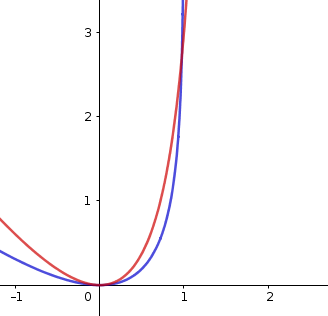
\includegraphics[width=8cm]{-ln-x} % leia abaixo
\caption{Em azul temos $-\log(1-x)-x$ e em vermelho $  \dfrac{x^2}{1-2x/3}$. }
\end{figure}
 







\bibliographystyle{alpha}

\bibliography{references}\nocite{*}


\newpage

\printindex





\end{document}
